%\documentclass[journal]{IEEEtran}
%\documentclass[10pt,journal,compsoc]{IEEEtran}
%\documentclass[10pt,journal,compsoc]{IEEEtran}
%\documentclass[journal,comsoc]{IEEEtran}
\documentclass[preprint]{elsarticle}
\pdfoutput=1
\usepackage{epsfig}
\usepackage{subfigure}
\usepackage{calc}
\usepackage{amssymb}
\usepackage{amstext}
\usepackage{amsmath}
\usepackage{amsthm}
\usepackage{pslatex}
\usepackage{url}
\usepackage[small]{caption}
\usepackage{todonotes}

\usepackage{enumerate} %enumerate with 1. 2. etc.

% ========= package for rotating table =======
\usepackage{lscape} 

% ======= following packages used for generating pseudocode of algorithms 
\usepackage{algorithm}
\usepackage{algorithmicx}
\usepackage{algpseudocode}
\usepackage{pifont}
%===================

% ======= package for degree sign ==========
\usepackage{gensymb}

%===== package for adding biography images =========
\usepackage{graphicx}
\graphicspath{ {bioimages/} }

%======== package for creating the table =================
\usepackage{tabularx,ragged2e,booktabs}
%\newcolumntype{L}{>{\RaggedRight\arraybackslash}X} % ragged-right version off "X"

% ======== package for creating coloured columns in tables.. ==========
\usepackage{xcolor,colortbl}

\subfigtopskip=0pt
\subfigcapskip=0pt
\subfigbottomskip=0pt

\journal{Big Data Research}

\begin{document}

\begin{frontmatter}

%% ======= TITLE =========f

%\title{RAIDS: Real-time Anomaly-based Intrusion Detection System for Cloud Data Centres}
%\title{ADDoSS: Anomaly-based DDoS Attack Detection System}
%\title{Reducing False Positives in DDoS Attack Detection}
\title{RADS: Real-time Anomaly Detection System for Cloud Data Centres}
%\title{\LARGE RADS: Real-time Anomaly Detection System for Cloud Data Centres}


%% ======= AUTHORS =========
%\author{Sakil Barbhuiya, Zafeirios Papazachos, Peter Kilpatrick and Dimitrios S. Nikolopoulos
%\IEEEcompsocitemizethanks{\IEEEcompsocthanksitem S. Barbhuiya, Z. Papazachos, P. Kilpatrick, and D. S. Nikolopoulos are with 
%the School of Electronics, Electrical Engineering and Computer Science, Queen's University Belfast, Belfast, United Kingdom.
%Email: \{sakil.barbhuiya, z.papazachos, p.kilpatrick, d.nikolopoulos\}@qub.ac.uk}}

\author[1]{Sakil~Barbhuiya\corref{cor1}}
\ead{sakil.barbhuiya@qub.ac.uk}

\author[1]{Zafeirios~Papazachos}
\ead{z.papazachos@qub.ac.uk}

\author[1]{Peter~Kilpatrick}
\ead{p.kilpatrick@qub.ac.uk}

\author[2]{Dimitrios~S.~Nikolopoulos}
\ead{dsn@vt.edu}

\cortext[cor1]{Corresponding author}
\address[1]{Queen's University Belfast, United Kingdom}
\address[2]{Virginia Tech, United States\\ }


%% ======= ABSTRACT =========
%\IEEEtitleabstractindextext{
\begin{abstract}
Cybersecurity attacks in Cloud data centres are increasing alongside the growth of the Cloud services market. 
%Cloud security attacks are increasing alongside the growth of the Cloud services market. 
Existing research proposes a number of anomaly detection systems for detecting such attacks. 
%These anomaly-based IDSs encounter a number of challenges, specifically due to the unknown behaviour of the attacks and the occurrence of genuine Cloud workload spikes, which must be distinguished from attacks. 
However, these systems encounter a number of challenges, specifically due to the unknown behaviour of the attacks and the occurrence of genuine Cloud workload spikes, which must be distinguished from attacks. 
In this paper, we discuss these challenges and investigate the issues with the existing Cloud anomaly detection approaches. Then, we propose a Real-time Anomaly Detection System (RADS) for Cloud data centres, which uses a one class classification algorithm and a window-based time series analysis to address the challenges. 
Specifically, RADS can detect VM-level anomalies occurring due to DDoS and cryptomining attacks.
%Specifically, RADS can detect DDoS and backdoor channel attacks in a Cloud data centre. 
%which can detect anoma- lies occurring due to DDoS and cryptomining attacks. 
%real-time with high accuracy and low false positive rates. 
%We evaluate the performance of RAIDS both in real-time and offline. The real-time evaluation was performed in a lab-based Cloud data centre whereas the offline evaluation was carried out with real-world Cloud workload traces.  
We evaluate the performance of RADS by running lab-based experiments and by using real-world Cloud workload traces. %The lab-based experiments were performed in an OpenStack based Cloud data centre.
%Real-world Cloud workload traces were collected from an online repository  
Evaluation results demonstrate that RADS can achieve 90-95\% accuracy with a low false positive rate of 0-3\%.
%The results further reveal that RADS experiences fewer false positives while using the proposed data pre-processing approach than when using state-of-the-art average or entropy based data pre-processing approaches.
The results further reveal that RADS experiences fewer false positives when using its window-based time series analysis in comparison to using state-of-the-art average or entropy based analysis.



\end{abstract}

%% ======= KEYWORDS =========
\begin{keyword}
Cloud, Anomaly Detection, Cybersecurity Attack, One Class Classification
\end{keyword}

\end{frontmatter}

%% ======= SECTIONS  =========f

\section{Introduction}
\label{sec:introduction}
\noindent The internet has become the dominant means of providing customer/citizen services for almost all business and government organisations. This is because of the advancement of Information and Communications Technology (ICT) mainly in the form of high speed internet connection, cloud computing services, and mobile devices. The growth of such internet-based or web-based services has attracted many cybersecurity attacks, which exploit the vulnerability of these services with evil intention. One of the major classes of cybersecurity attacks is the Distributed Denial of Service (DDoS) attack, which deny legitimate customers' access to the web-based services. Typically, DDoS attacks are launched by sending a redundant stream of network packets from a large number of compromised computer systems and/or mobile devices. 
%In most cases, the victims of such attacks are the prominent websites. 
The number of DDoS attacks and their volume have been increasing for the last few years. According to a report~\cite{coreo2} from Corero, in 2019, there was 35\% increase in DDoS attacks over 10Gbps as compared to 2018. This year, due to the COVID-19 pandemic people have turned to using the internet like never before - people are studying, working, shopping, and having fun online. This has shifted the gear of DDoS attacks - the new targets are websites of medical organisations, delivery services, educational, and gaming platforms. The impact of this can be observed in the latest DDoS attacks trend~\cite{kas} published by Kaspersky Lab: the number of DDoS attacks in Q1 2020 increased by 80\% against Q1 2019.  
%their customers experienced on average 8 DDoS attacks per day, which is 16\% more as compared to 2017. Also, the report reveals that in early 2018, the two largest-ever DDoS attacks hit the Github website (1.35 Tbps attack) and an unnamed US-based service provider (1.7 Tbps attack).
%The number of DDoS attacks and their volume have been increasing for the last few years. According to a report~\cite{coreo} from Corero, in 2018, their customers experienced on average 8 DDoS attacks per day, which is 16\% more as compared to 2017. Also, the report reveals that in early 2018, the two largest-ever DDoS attacks hit the Github website (1.35 Tbps attack) and an unnamed US-based service provider (1.7 Tbps attack).

To launch a successful attack, DDoS attacks must significantly consume network bandwidth. This results in an obvious change in the network traffic pattern or in the network packet information, which can be seen as network anomalies. Researchers have used various techniques such as~\cite{automated-detection:2016, UBL:2012, cloud-malware:2016} to detect network anomalies.
%, which include using machine learning and statistical approaches. 
%The anomaly detection systems proposed in~\cite{ml_based:2012, Pandeeswari2016, ML_based_ids:2016} use supervised machine learning algorithms. These algorithms require both the ``normal" and the ``anomalous" behaviour traces to build the learning models, which can detect the anomalies. 
%In a Cloud data centre, ``normal" traces can be prepared easily by monitoring the VMs' resource utilisation in the situation where the VMs are believed to be anomaly-free; however, ``anomalous" traces need to be generated artificially using emulation or collected from online repositories. 
%The algorithms may fail to detect anomalies arising due to unknown DDoS attacks, traces of which are not recorded by the learning models or which have very different patterns from the learned ``anomalous" patterns. 
%To solve this problem 
%To detect Researchers in~\cite{automated-detection:2016, UBL:2012, cloud-malware:2016} have proposed 
Specifically, they have used unsupervised learning and one class classification algorithms such as K-Means~\cite{automated-detection:2016}, Self Organising Map (SOM)~\cite{UBL:2012} , and one class Support Vector Machine (SVM)~\cite{cloud-malware:2016}. 
These algorithms first build the learning models by using normal network traffic or packet information and then use these models to identify anomalies by observing the deviation from the normal traffic pattern or packet information. 
Recently, entropy has been used in various network anomaly detection systems~\cite{entorpy_based_detection_5:2014}, \cite{entorpy_based_detection_3:2017}, \cite{entorpy_based_detection_4:2017}. These systems firstly measure the entropy associated with the network traffic or network packet features (IP addresses and ports), and secondly they detect network attacks by observing the anomalies in the entropy values.
%These algorithms build the learning models by using the ``normal" behaviour traces. The models can identify anomalies by observing the deviation in the ``normal" behaviour pattern. 
%and as a result, these algorithms can successfully detect zero-day or unknown attacks.
%These algorithms learn only from the ``normal" behaviour traces and do not use the ``anomalous" traces, and as a result, they can successfully detect zero-day or unknown attacks which impose significant deviation in the ``normal" behaviour pattern. 

%Although the techniques as mentioned above can detect network anomalies with high accuracy, they may exhibit false positives arising due to network traffic spikes. We can consider these spikes as "legitimate spikes" which do not follow the ``normal" traffic pattern and their values are significantly higher than the other values in the traffic data set. 
Although the techniques as mentioned above can detect network anomalies with high accuracy, they exhibit false positives, that is they generate anomaly alarms when there is no anomaly. Receiving such false alarms on a frequent basis is a major demerit of anomaly detection systems for a number of reasons: waste of operators' time as they engage in unnecessary investigations of the falsely raised alarms, unwanted interruption of services while the operator tries to mitigate the anomaly without realising that the alarm is false, etc. To investigate the cause for such false positives, we carried out a linear classification analysis of the network traffic collected from a real Cloud data centre trace~\cite{workloadCCGRID:2015} and a DDoS attack sample~\cite{caida}. 
%The reason for choosing the linear classification is that state-of-the-art anomaly-based techniques use such classification to detect DDoS attacks. 
%We performed this test analysis graphically by drawing the classification hyperplanes around the traffic data points. 
Our investigation suggested that traffic spikes play a significant role in generating false positives. We define these spikes as legitimate activity which does not follow the normal traffic pattern and their values are significantly higher than the other values in the traffic data. 
%As we investigated arising due to network traffic spikes. We can consider these spikes as "legitimate spikes" which do not follow the ``normal" traffic pattern and their values are significantly higher than the other values in the traffic data set. 
It is important to note that these spikes persist only for a momentary period of time and this differentiates them from the network anomalies (high network traffic) due to DDoS attacks, which persist for a relatively long period of time. We support this argument with evidence from real-world network traffic and DDoS attack. 
%Receiving false positive alarms on a frequent basis is a major demerit of anomaly detection systems for a number of reasons: waste of operators' time as they engage in unnecessary investigations of the falsely raised alarms, unwanted interruption of customers' services while the operator tries to mitigate the anomaly without realising that the alarm is false, etc. 
%This motivates a solution to remove false positives from the network anomaly detection systems. 
%Researchers in~\cite{automated-detection:2016}, \cite{UBL:2012}, \cite{cloud-malware:2016} consider window-based averaging on the raw data to reduce false positives. The works in~\cite{EbAT:2010} and \cite{entorpy_based_detection_2:2014} consider entropy-based anomaly detection which also reduces the number of false positives. However, these approaches may still generate false positives due to network traffic spikes, which we explain in the next section.
%Researchers in~\cite{automated-detection:2016}, \cite{UBL:2012}, \cite{cloud-malware:2016} use averaging on the raw data as a data pre-processing approach to reduce false positives. The works in~\cite{EbAT:2010} and \cite{entorpy_based_detection_2:2014} consider entropy analysis in their anomaly detection systems which also reduces the number of false positives. However, these approaches may still generate false positives in certain scenarios for certain use cases, which we explain in the next section.

To deal with the traffic spikes and to reduce the false positives, in this paper, we propose a linear regression based DDoS attack detection technique. The technique is based on the hypothesis that there is a positive correlation between average and standard deviation of the network throughput in a window-based time series, and this correlation is affected due to DDoS attacks. The hypothesis is supported by the findings in~\cite{variance}.
%ADDoSS works in two phases, the training phase and the detection phase. 
The proposed technique works in two phases: training and detection. During the training phase, it builds a linear regression model using the average and standard deviation values of the network throughput. During the detection phase, for a particular detection window, it firstly uses the linear regression model to predict the standard deviation of the network throughput for the given (measured) average value and secondly, it calculates the difference between the predicted and the measured standard deviation values in order to identify whether there is any anomaly in the detection window. 

Specifically, we make the following contributions in this paper:
\begin{enumerate}[{(1)}]
%\item RAIDS provides an algorithm based on probabilistic classification for detecting anomalies in cloud applications. The accuracy of the algorithm is examined using different virtual machines running various services from the CloudSuite workload collection. The proposed algorithm utilises probability distribution analysis on the raw data (??) to detect anomalies and minimise false positives.
%\item \textcolor{red}{We propose a new intrusion detection algorithm for Cloud that provides high accuracy and low false positives in detecting Cloud security attacks such as DDoS and backdoor channel attacks.}
\item We propose a linear regression based technique for detecting DDoS attacks with high accuracy and crucially low false positive rate. 
\item We evaluate the performance of the proposed technique by running experiments on real-world network traffic (collected from a Cloud data centre named Bitbrains~\cite{bitbrains} and CAIDA DDoS attack 2007 dataset~\cite{caida}. 
\item We compare the proposed technique against average and entropy based one class classification (OCC)~\cite{OCC:2008} techniques, which represent the state-of-the-art linear classification techniques to detect DDoS attacks. 
\end{enumerate}

%Evaluation results demonstrate that the proposed linear regression based technique reduces the false positive rates significantly while maintaining the accuracy of attack detection. The remainder of the paper is organised as follows. Section~\ref{sec:problem_definition} describes the problems with the existing approaches in DDoS attack detection. Section~\ref{sec:related_work} presents related work in network anomaly detection.
Evaluation results demonstrate that the proposed linear regression based technique reduces the false positive rate by 95\% and 99\% when compared against average and entropy based OCC techniques, respectively, while maintaining the accuracy of attack detection (92\%, which is 18\% and 114\% better than average and entropy based OCC techniques, respectively). 

The remainder of the paper is organised as follows. Section~\ref{sec:preliminary_investigation} investigates the issues with the existing DDoS attack detection techniques. 
Section~\ref{sec:proposed_technique} formulates the hypothesis and proposes the DDoS attack detection technique. 
Section~\ref{sec:evaluation} presents experimental results and discusses them. 
Section~\ref{sec:related_work} discusses the related work in network anomaly detection.
Finally, Section~\ref{sec:conclusions} concludes the paper. 

\section{Problem Definition}
\label{sec:problem_definition}
%\todo[author=DSN,inline]{Can we refrain from referring to Challenges and attacks as 'Challenge 1-2-3', 'Attack 1-2-3'? We can give abbreviations to them and use the abbreviations throughout the paper. Otherwise it is hard for the reader to remember what 1-2-3 stands for.}
%\todo[author=SB,inline]{Changed the numberings to names, please check!}
%\noindent Researchers in ~\cite{cloud-malware:2016}, \cite{automated-detection:2016}, \cite{UBL:2012} attempt to address \textit{challenge 1} by proposing unsupervised and semi-supervised machine learning algorithms such as K-Means, Self Organising Map (SOM) algorithms, and one class Support Vector Machine (SVM). 
%They also use averaging on the raw data as a data pre-processing step to address \textit{challenge 2}.
%Researchers in~\cite{EbAT:2010}, \cite{entorpy_based_detection_2:2014}, \cite{density-based:2016} consider data distribution (entropy and density) to solve \textit{challenge 1} and \textit{challenge 2}.
%They also use averaging on the raw data as a data pre-processing step to address \textit{challenge 2}. Researchers in~\cite{EbAT:2010} and \cite{entorpy_based_detection_1:2005} consider data distribution (entropy and density) to solve \textit{challenge 1} and \textit{challenge 2}. 
%Although these approaches help intrusion detection systems (IDSs) to achieve high accuracy with low false positive rates, they may suffer from accuracy and false alarm issues in certain scenarios for certain use cases.  
%To demonstrate this, 
%In order to showcase how state-of-the-art anomaly-based IDSs for Cloud may encounter accuracy and false alarm issues, we created a scenario where a Cloud application runs in one of the VMs in a Cloud data centre and at one stage the application suffers from a backdoor channel attack that increases its resource utilisation, specifically, the CPU utilisation. We built the Cloud data centre in our lab using OpenStack\footnote{https://www.openstack.org} (details of the set-up are available in Section~\ref{sec:experiments}) and executed one Graph Analytics workload (collected from CloudSuite\footnote{http://cloudsuite.ch}) as the Cloud application in one of the VMs hosted in our lab-based Cloud data centre. 
%In this section we showcase how the state-of-the-art average~\cite{automated-detection:2016}, \cite{UBL:2012}, \cite{cloud-malware:2016}, and entropy~\cite{EbAT:2010}, \cite{entorpy_based_detection_2:2014} based data analysis may result in low accuracy and high false positive rate for anomaly detection systems in the Cloud.  In addition, we show how standard deviation based analysis may also raise accuracy and false positive issues.
%In this section we give a brief summary on how anomaly detection systems generally work in detecting cybersecurity attacks in the Cloud. Then, we highlight the underlying assumptions of such Cloud anomaly detection systems and define their key problems.  
%In this section we give a brief summary on how anomaly detection systems generally work in detecting cybersecurity attacks in the Cloud. Then, we define the key problems with these systems. 
\noindent In order to detect cybersecurity attacks in a Cloud data centre, anomaly detection systems generally make the following assumptions:
\begin{itemize} %[{(1)}] 
\item \textbf{Assumption-1:} Resource utilisation of a VM follows some kind of ``normal” behaviour or trend which can be modelled by using machine learning or statistical approaches.
\item \textbf{Assumption-2:} Cybersecurity attacks such as DDoS and crytomining attacks consume VM resources significantly. This results in a deviation in the ``normal” trend of a VM's resource utilisation, which can be captured as anomalous by the machine learning or statistical approaches.
%which can be captured as anomaly by the machine learning or statistical approaches. 
\end{itemize} %[{(1)}] 

Assumption-1 is very general and is considered by many anomaly detection systems like~\cite{automated-detection:2016}, \cite{UBL:2012}, \cite{cloud-malware:2016}, \cite{EbAT:2010}. 
%Assumption-2 is also considered by researchers in [] specifically for DDoS attacks. We find evidence of the impact of cryptomining attacks on CPU in these [REF] related work.  
Assumption-2 is experimentally demonstrated by~\cite{ddso_charater_2017} while they analysed real DDoS attack samples taken from the CAIDA\footnote{http://www.caida.org/data/passive/ddos-20070804\_dataset.xml} dataset. 
%A recent report\footnote{https://www.prnewswire.com/news-releases/radiflow-reveals-first-documented-cryptocurrency-malware-attack-on-a-scada-network-300595714.html} published by PR Newswire announces that 
%A recent report\footnote{https://www.prnewswire.com/news-releases/radiflow-reveals-first-documented-cryptocurrency-malware-attack-on-a-scada-network-300595714.html} announces that 
Recently, Radiflow\footnote{https://radiflow.com}, a cybersecurity solution provider, has discovered the first documented cryptomining attack on a SCADA network. According to Radiflow, cryptomining attacks cause high CPU and network bandwidth consumption. 
In our work, we also consider both these assumptions.
%Radiflow\footnote{https://radiflow.com} announces that has revealed the first documented cryptocurrency malware attack on a SCADA network of a critical infrastructure operator. that ,  We find evidence of the impact of cryptomining attacks on CPU in these [REF] related work.  

%\textcolor{red}{In most cases, the Cloud anomaly detection systems perform well under these assumptions, but, however, there are some cases where they may suffer from performance issues. We explain this in the following example: }
% how the state-of-the-art average~\cite{automated-detection:2016}, \cite{UBL:2012}, \cite{cloud-malware:2016}, and entropy~\cite{EbAT:2010}, \cite{entorpy_based_detection_2:2014} based data analysis may result in low accuracy and high false positive rate for anomaly detection systems in the Cloud.  In addition, we show how standard deviation based analysis may also raise accuracy and false positive issues.
%fail to differentiate genuine Cloud workload spikes from ``anomalous" behaviour and generate false positive whenever they encounter such spikes.  

In most cases, the Cloud anomaly detection systems perform well under these assumptions. However, there are some cases where they may suffer from performance issues. In this paper we specifically consider the case where a Cloud anomaly detection system is using a linear classifier like K-Means, SVM, Naive Bayes, etc., and the VMs are exhibiting workload spikes. We explain this in the following example.

\textit{Example Scenario:} We created an example scenario where a VM hosted in a Cloud data centre runs a Cloud application and at one stage the VM becomes compromised by a cryptomining attack that consumes its CPU to perform illicit cyrptocurrency mining. We built the Cloud data centre in our lab using OpenStack\footnote{https://www.openstack.org} (details of the set-up are available in Section~\ref{sec:experiments}) and executed a Graph Analytics workload (collected from CloudSuite\footnote{http://cloudsuite.ch}) as the Cloud application in one of the VMs hosted in our data centre. 
We emulated the cryptomining attack by running a CPU stress tool that consumes almost 100\% CPU of the VM. This emulation closely relates to real-world cryptomining attacks where the CPUs are consumed significantly to perform the mining. 
%Further, we injected some artificial instantaneous spikes by running the CPU stress tool for instantaneous period of time consecutively. 
%Details of the testbed and the data collection for the experiment are available in Section~\ref{sec:experiments}. 
%carried out a preliminary experiment in our lab-based cloud data centre or testbed (details of the testbed are available in Section~\ref{sec:experiments}). Details of the testbed and the data collection for the experiment are available in Section~\ref{sec:experiments}. 
%We applied different statistical measurements such as average, standard deviation, and entropy on the raw CPU utilisation data collected from running the cloud application. 
Considering this scenario, we performed 10 minutes of experiment to analyse the VM's CPU utilisation under different situations. 
We split the experimental period into two - (i) \textit{normal-period}: first 5 minutes, without any attack and (ii) \textit{anomaly-period}: last 5 minutes, under cryptomining attack. 
%To complete the scenario, we injected some artificial workload spikes during the 3\textsuperscript{rd} minute by running the CPU stress tool for instantaneous periods of time consecutively. 
Furthermore, we injected some artificial workload spikes during the 3\textsuperscript{rd} minute by running the CPU stress tool for instantaneous periods of time consecutively. 
Figure~\ref{fig:cpu_timeseries} presents the time series graph of the CPU utilisation collected every 5 seconds. 

% APPROACH CPU TIMESERIES 
%\vfill
\begin{figure}[!h]
  %\vspace{-0.2cm}
  \centering
   {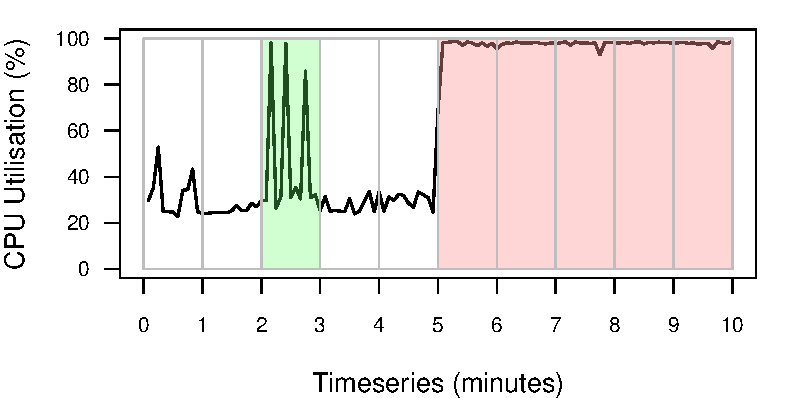
\epsfig{file = figures/approach_cpu_timeseries, width = 0.8\columnwidth}}
   \caption{Time series of CPU utilisation while running the Graph Analytics application. Pink coloured sections represent the utilisation during the \textit{anomaly-period} and green coloured section represents the utilisation with workload spikes during the \textit{normal-period}}
  \label{fig:cpu_timeseries}
  %\vspace{-0.1cm}
\end{figure}
%\vfill

% APPROACH CPU AVG, ENTROPY, SD 
%\vfill
\begin{figure}[!h]
  %\vspace{-0.2cm}
  \centering
   {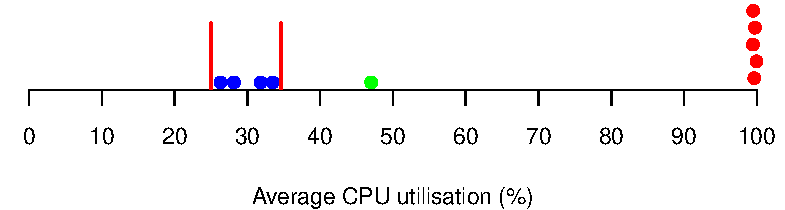
\epsfig{file = figures/approach_avg_dot, width = 0.8\columnwidth}}
     \hspace{0.9cm}
      {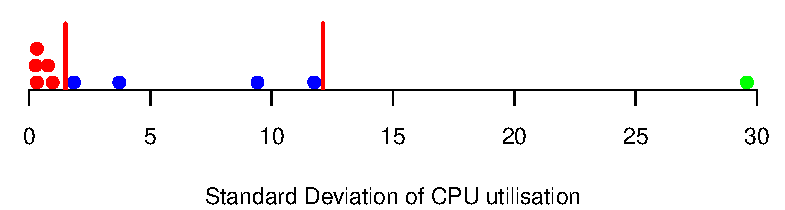
\epsfig{file = figures/approach_sd_dot, width = 0.8\columnwidth}}
        \hspace{0.9cm}
         {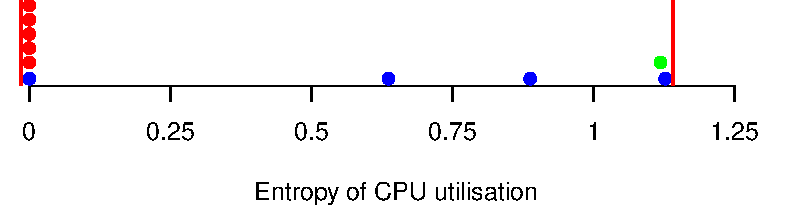
\epsfig{file = figures/approach_entropy_dot, width = 0.8\columnwidth}}
   \caption{Average, standard deviation, and entropy of CPU utilisation}
  \label{fig:avg_sd_entropy}
  %\vspace{-0.1cm}
\end{figure}
%\vfill

%\todo[author=DSN,inline]{It is not immediately clear what data processing techniques you are referring to here. Have you defined them or cited them earlier in the paper?}
%\todo[author=SB,inline]{Cited them now here, please check}
\textit{Window-based Time Series Analysis:} 
%Both the average and the entropy based time series analysis used in the Cloud anomaly detection systems such as~\cite{automated-detection:2016}, \cite{UBL:2012}, \cite{cloud-malware:2016}, \cite{EbAT:2010}, \cite{entorpy_based_detection_2:2014} are window-based, where the raw data are firstly distributed into a number of data bins with equal window size and secondly, the average or entropy of the data is calculated in each bin. These averages or entropies collected from the bins form the time series data to be used in the anomaly detection systems. 
%To produce the window-based time series data, we grouped the CPU utilisation data points into 10 data bins, each with a window size of 1 minute (the grey coloured partitions of the timeseries in Figure~\ref{fig:cpu_timeseries}) and then calculated three statistical measurements (average, standard deviation, and entropy) of the CPU utilisation in each bin. We selected the window size to be 1 minute as we experimentally found that anything shorter than this does not help in reducing the noise or spikes from the CPU utilisation and anything longer than this does not capture the short-term CPU utilisation behaviour.  
Anomaly detection systems which use linear classifiers, generally perform window-based time series analysis where the raw time series data are firstly distributed into a number of data bins with equal window size, and secondly, the average or entropy of the data is calculated in each bin. These averages or entropies collected from the bins form the time series data to be used in the anomaly detection systems.
To perform such an analysis, we grouped the CPU utilisation data points into 10 data bins, each with a window size of 1 minute (the grey coloured partitions of the time series in Figure~\ref{fig:cpu_timeseries}) and then calculated three statistical measurements (average, standard deviation, and entropy) of the CPU utilisation in each bin. We selected the window size to be 1 minute as we experimentally found that anything shorter than this does not help in reducing the noise from the CPU utilisation and anything longer than this does not capture the short-term CPU utilisation behaviour.  
%\textcolor{red} {We calculated the entropy using the equation ...}
%\textcolor{red}{Entropy [29] is calculated using the equation~\ref{eq1}. }%is a widely used measurement that captures the degree of dispersal or concentration of random variable distributions. 

For a discrete random variable $X$ with possible values $\big\{x_1,x_2...,x_n\big\}$ the entropy~\cite{entropy:2001} is calculated using Equation~\ref{entropy}. 
To prepare the data for the entropy calculation in each bin, we firstly normalise each of the raw data samples using Equation~\ref{normalisation} (normalised values are in the range $[0.0-1.0]$) and secondly, we decide to which amongst the following 10 smaller bins each normalised value belongs: 
$[0.0-0.1), [0.1-0.2), [0.2-0.3), [0.3-0.4), [0.4-0.5), [0.5-0.6), [0.6-0.7), [0.7-0.8), [0.8-0.9), [0.9-1.0]$. 
Finally, in each bin, we count the number of occurrences of the normalised values of the raw data samples in each smaller bin.
Thus, in Equation~\ref{entropy} we consider these numbers of occurrences as the values of the random variable $X$ in order to calculate the entropy.

We had 10 values (1 from each data bin) for each statistical measurement, which we present in Figure~\ref{fig:avg_sd_entropy} using 10 coloured dots along the x-axis. The 4 blue dots represent the measurements during the \textit{normal-period}, whereas the 5 red dots represent the measurements during the \textit{anomaly-period}. The green dot represents a measurement during the \textit{normal-period}, when the CPU encountered consecutive workload spikes (refers to the 3\textsuperscript{rd} minute in Figure~\ref{fig:cpu_timeseries}).

\begin{equation}
\label{entropy}
H(X) = -\sum\limits_{i=1}^n P(x_i)\log P(x_i)
\end{equation}
\begin{tabular}{l l}
     where &$P(x_i)$\;=\;probability mass function of $x_i$\\
                &$-logP(x_i)$\;=\;surprisal or self-information of $x_i$\\
\end{tabular}\\ 

\begin{equation}
\label{normalisation}
    X_{normalised} \quad = \quad   \frac{X - X_{min}}{X_{max} - X_{min}}
\end{equation}
\begin{tabular}{l l}
     where &$X_{normalised}$\;=\;normalised metric value\\
                &$X$\;=\;current metric value\\
                &$X_{min}$\;=\;minimum metric value in the raw data set \\
                &$X_{max}$\;=\;maximum metric value in the raw data set \\
\end{tabular}\\ \\ 

%In an ideal case of a linear classifier, we expected that the blue and the green dots are separable from the red dots by a hyperline. But, the measurements from Figure~\ref{fig:avg_sd_entropy} show different results. 
%From Figure~\ref{fig:avg_sd_entropy} we observe that, in the case of average, although the blue and the red dots are clearly separable by using a hyperline (the red line), the green dot falls on the wrong side of the hyperline. In case of standard deviation and entropy, we observe that even the blue and the red dots are not separable by any hyperline, instead the green dot becomes separable from both of them. 
%In an ideal case of an unsupervised learning or one class classifier, we expect that the blue and the green dots (normal behaviour data points) are clustered together in such a way that they are separable from the red dots (anomaly behaviour data points) by hyperplanes. But, the measurements from Figure~\ref{fig:avg_sd_entropy} show different results. 
%In case of unsupervised learning~\cite{automated-detection:2016}, \cite{UBL:2012} or one class classification~\cite{cloud-malware:2016} algorithms, the normal data points are clustered together and surrounded by hyperplanes and any data point outside those hyperplanes is considered as anomaly. For each statistical measurement, we tried to cluster the normal data points (blue and green dots) together and draw the hyperplanes (the red lines) surrounding them (see Figure~\ref{fig:avg_sd_entropy}). 
In the case of linear classifiers, the ``normal" data points are separated from the ``anomalous" data points by a hyperplane. 
%For each statistical measurement, we tried to cluster the normal data points (blue and green dots) together and draw the hyperplane (the red lines) to separate them from the anomalies (red dots) (see Figure~\ref{fig:avg_sd_entropy}). 
%For each statistical measurement, we considered that the anomalies (red dots) the genuine workload spikes (green dot) are appearing only during the testing or detection phase of the classifier and therefore, we tried to draw the hyperplane (the red lines) only considering the normal data points (blue dots) (see Figure~\ref{fig:avg_sd_entropy}). 
In this analysis, we consider that the anomalies (red dots) and the genuine workload spikes (green dot) are appearing only during the testing or detection phase of the classifier. Therefore, for each statistical measurement, we drew two hyperplanes (the red lines) by considering the minimum and the maximum values of the ``normal" data points (blue dots); Figure~\ref{fig:avg_sd_entropy} presents this. We expected that the green dot (workload spikes) resides within the hyperplanes as they belong to the \textit{normal-period} and the red dots (anomalies) are clearly separable by the hyperplanes as they belong to the \textit{anomaly-period} of the experiment. 
%red dots (anomalies) reside outside the hyperplanes as they belong to the \textit{anomaly-period} of the experiment.
%In case the genuine workload spikes are occurring during the training phase then using only approach (a) will suffice as in that case, the spike samples can be recorded as ``normal" by OCC algorithm. But, if the genuine workload spikes are not seen during the training phase and they are only appearing during the testing or the detection phase then we need to use both approach a and b. We consider the latter condition in our experimental evaluation.
%presents the classification amongst the blue, red, and green dots. But, we found that the green dot representing the genuine workload spikes resides outside the hyperplanes as it is far from the cluster of blue dots.
%From the figure we observe that, in case of average, the blue dots are closely clustered and the green dot representing the genuine workload spikes is far from this cluster and hence, it resides outside the hyperplane, indicating an anomaly.
%In case of standard deviation, although the blue dots are clustered together, the blue and the red dots are marginally separable by the left hyperplane, and importantly, the green dot moves very far from both the blue and the red dots.
%However, from the figure we observe that, in case of average, the blue dots are closely clustered and clearly separable from the red dots by the right hyperplane. However, the green dot representing the genuine workload spikes is far from the cluster of blue dots and hence, it resides outside the hyperplanes, indicating an anomaly.
%In case of standard deviation, although the blue dots are clustered together, the blue and the red dots are marginally separable by the left hyperplane, and importantly, the green dot moves very far from both the blue and the red dots.
From the figure we observe that, in the case of average, the blue dots are closely clustered and the red dots are clearly separable from them by the right hyperplane. However, the green dot representing the genuine workload spikes does not reside within the hyperplanes and indicates an anomaly.
In the case of standard deviation, although the blue dots are clustered together, the blue and the red dots are marginally separable by the left hyperplane, and importantly, the green dot does not reside within the hyperplanes and moves very far from both the blue and the red dots.
%outcome of which is discussed as follows: 
%they are separable from the red dots (anomaly behaviour data points) by hyperplanes. But, the measurements from Figure~\ref{fig:avg_sd_entropy} show different results. 
%From Figure~\ref{fig:avg_sd_entropy} we observe that, in case of average, although the blue and the red dots are clearly separable by using hyperplanes (the red lines), the green dot resides outside the hyperplanes as it is far from the cluster of blue dots.
%In case of standard deviation, we observe that the blue and the red dots are marginally separable by the hyperplanes and importantly, the green dot moves very far from both the blue and the red dots.
%In case of entropy, the blue dots are not clustered together and they are mixed with the red dots.
In the case of entropy, the blue and the red dots are not separable, although the green dot resides within the hyperplanes.
%even the blue and the red dots are not separable by any hyperplane.
From these observations we identify the following problems for Cloud anomaly detection systems:
\begin{enumerate}[{(1)}] 
%\item An average based linear classifier cannot differentiate between the ``normal" and the ``anomalous" VM resource utilisation behaviour if the VM encounters workload spikes. Specifically, they may wrongly identify the genuine Cloud workload spikes as anomalies and raise false positives.
\item An average based linear classifier may identify the genuine workload spikes as anomalies and raise false positives.
%\item Similar to average, a standard deviation based linear classifier may also raise false positives; additionally, it may even fail to identify anomalies and raise false negatives resulting in low detection accuracy.  
\item Similar to average, a standard deviation based linear classifier may also raise false positives. Additionally, it may even fail to differentiate between normal behaviour and anomalies, which may raise false negatives resulting in low classification accuracy.  
\item An entropy based linear classifier may not raise false positives; but, similar to standard deviation, it may result in low classification accuracy due to failure in differentiating between normal behaviour and anomalies.
%between the ``normal" and the ``anomalous" VM resource utilisation behaviour: in fact entropy based classifier fails even when the normal behaviour does not include workload spikes. Hence, they may fail to identify the anomalies and raise false negatives resulting into low detection accuracy. 
%\item Similar to average, standard deviation and entropy based linear classifiers also fail to differentiate between the ``normal" and the ``anomalous" VM resource utilisation behaviour: in fact entropy based classifier fails even when the normal behaviour does not include workload spikes. Hence, they may fail to identify the anomalies and raise false negatives resulting into low detection accuracy. 
%\begin{itemize}
%\item The average values cannot differentiate between the ``normal" and the ``anomalous" Cloud application behaviour if the normal behaviour encounters workload spikes. Specifically, any average based linear classifier may wrongly identify the genuine workload spikes as anomalies, which will increase the false alarms. 
%\item Similar to average, standard deviation and entropy fail to differentiate between the ``normal" and the ``anomalous" Cloud application behaviour: in fact they fail even when the normal behaviour does not have any workload spikes. Hence, any standard deviation and entropy based linear classifier may struggle to identify the anomalies due to security attack, which will reduce detection accuracy. 
%\item The average values cannot differentiate between the normal and the anomalous cloud application behaviour if the normal behaviour encounters instantaneous spikes. Specifically, if the spikes appear only during the testing or the detection phase and not during the training phase, then the classifier may wrongly identify the spikes as anomalies, which will increase the false alarms. 
%On one hand, if the spikes appear during the training period of an average based linear classifier, then the classifier may not successfully identify the anomalies, which will reduce the detection accuracy. On the other hand, if the spikes appear only during the testing or the detection phase, then the classifier may wrongly identify the spikes as anomalies, which will increase the false alarms. 
%\item Similar to average, standard deviation and entropy fail to differentiate between the normal and the anomalous cloud application behaviour, in fact they fail even when the normal behaviour does not have any instantaneous spikes. Hence, any  standard deviation and entropy based linear classifier may also suffer from accuracy and false alarm issues. 
\end{enumerate}
%\end{itemize}
%Researchers do not emphasise much on \textit{challenge 3}. They generally build the behavioural models with fixed training duration, which they usually decide based on offline experiments and they keep the duration constant throughout the intrusion detection process. Thus, they do not provide techniques to extract optimised duration for the training, which can be dynamically decided based on the online or real-time application resource utilisation pattern.
%\todo[author=DSN,inline]{This reads well but again, bares rather limited relevance to the Cloud. You could strengthen the motivation for this discussion by articulating that normal, non-anomalous spikes are a common behaviour in the Cloud. Ideally, you should back this claim up with citations.}
%\todo[author=SB,inline]{Please check the red texts in Introduction (in the discussion of challenges) where I have mentioned that spikes are more common in the Cloud with reference}

%\section{RADS Approach To Anomaly Detection}
\section{RADS Window-based Time-series Analysis}
\label{sec:approach}
\noindent 
%From the previous section, we observe an important point that the standard deviation resulted from the genuine workload spikes is significantly higher than the other standard deviation values. 
%This can be used as an indicator for the genuine workload spikes to not identify them as anomalies. 
%Based on this we propose a new approach to differentiate the anomalous behaviour due to attack from the normal behaviour. Our approach uses a combination of the volume (average) and the underlying distribution (standard deviation) of the raw data. 
%In this section we propose a new approach to differentiate a Cloud VM's ``anomalous" behaviour from its ``normal" behaviour. 
%The novelty of the approach lies in its ability to classify genuine Cloud workload spikes as ``normal" in order to remove false positives arising due to wrongly classifying spikes as ``anomalies".
%In this section we propose RADS approach to detect anomalies in the Cloud data centres. The key idea of this approach is to differentiate the genuine Cloud workload spikes from the “anomalies” in order to identify them as “normal” and remove false positives without compromising the accuracy of anomaly detection. This is achieved by considering the combination of the average and the standard deviation of the raw data. The idea stems from the following important observation from the previous section: average value of raw data measured during the workload spike situation is higher than the average values measured during the normal situation, which is accompanied by a very high standard deviation value (higher than the standard deviation values measured during the normal and the anomalous situations).
%In this section we propose RADS approach to detect anomalies in the Cloud data centres. 
%The novelty of this approach is its ability to differentiate the genuine Cloud workload spikes from the anomalies in order to reduce false positives without compromising the accuracy of anomaly detection. 
%To achieve this, RADS uses a window-based time series analysis which combines average and standard deviation of the raw data in each time series window; and uses artificial data points that represent workload spikes. 
%The idea stems from the following important observation from the previous section: 
%average value of raw data measured during the workload spike situation is higher than the average values measured during the normal situation, which is accompanied by a very high standard deviation value (higher than the standard deviation values measured during the normal and the anomalous situations). 
%This is achieved by considering the combination of the average and the standard deviation of the raw data. The idea stems from the following important observation from the previous section: \textit{average value of raw data measured during the workload spike situation is higher than the average values measured during the normal situation, which is accompanied by a very high standard deviation value (higher than the standard deviation values measured during the normal and the anomalous situations). }
%The novelty of the approach lies in its ability to classify between anomalies and genuine Cloud workload spikes in order to remove false positives arising due to wrongly identifying spikes as ``anomalies".
%The approach uses combination of the volume (average) and the underlying distribution (standard deviation) of the raw data. 
%The approach uses combination of the average and the standard deviation of the raw data. 
%COMBINATION OF AVG AND SD GRAPH
%\vfill
\begin{figure}[!h]
  %\vspace{-0.2cm}
  \centering
   {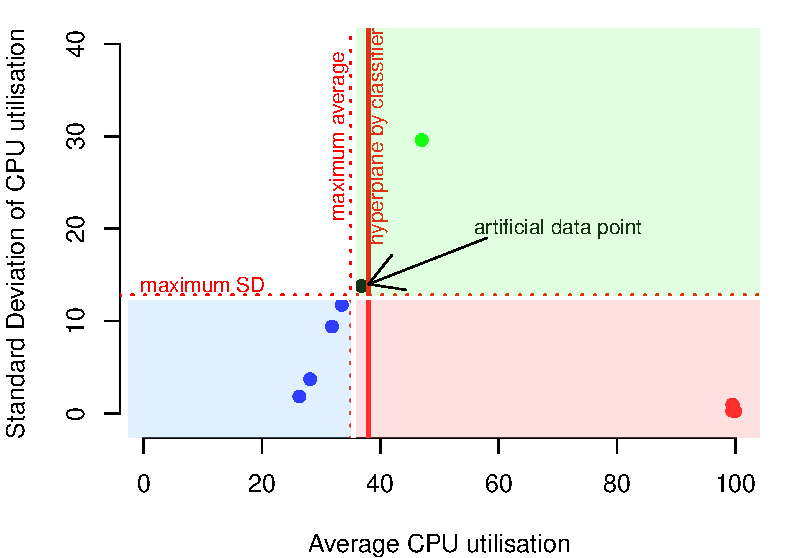
\epsfig{file = figures/approach_avg_sd_dot, width = 0.8\columnwidth}}
   \caption{RADS approach: combining average and standard deviation}
  \label{fig:avg_sd_combined}
  %\vspace{-0.1cm}
\end{figure}
%\vfill

\noindent In this section we explain RADS window-based time series analysis that resolves the problems identified in the previous section. 
%The novelty of this approach is its ability to differentiate the genuine Cloud workload spikes from the anomalies in order to reduce false positives without compromising the accuracy of anomaly detection. 
Specifically, RADS combines average and standard deviation of the raw data in each time series window; and uses artificial data points that represent workload spikes. 

If we combine the average and standard deviation values generated from the experiment as discussed in the previous section, then we can represent them in a two-dimensional space as shown in Figure~\ref{fig:avg_sd_combined}. Similar to the previous section, blue, red, and green dots refer to the measurements during the normal, anomalous, and spike situations, respectively. From the figure we observe that the coloured dots can be classified into three classes if we draw the dotted red hyperplanes (horizontal and vertical) based on the maximum average on x-axis and maximum standard deviation (SD) on y-axis. Hence, this becomes a three class classification problem, where the classes can be labeled as: ``normal'' (blue coloured section) containing blue dots, ``anomaly'' (pink coloured section) containing red dots, and ``spike'' (green coloured section) containing green dot. However, we do not wish to go in that direction of classification as we assume that the samples for the ``anomaly'' class as well for the ``spike'' class are not available or known. 
%\textbf{RADS window-based time-series analysis:} 
%Figure~\ref{fig:avg_sd_combined} presents coloured dots in a two-dimensional space to represent both average and standard deviation values of the CPU utilisation (collected from the experiment discussed in the previous section). Similar to the previous section, blue, red, and green dots refer to the measurements during the normal, anomalous, and spike situations, respectively. 
%demonstrates how the approach helps in solving the problems identified in the previous section. 
%From the figure we observe that the coloured dots can be classified into three classes if we draw the dotted red hyperplanes (horizontal and vertical) based on the maximum average on x-axis and maximum standard deviation (SD) on y-axis. Hence, this becomes a three class classification problem, where the classes can be labeled as: ``normal'' containing blue dots, ``anomaly'' containing red dots, and ``spike'' containing green dot. However, we do not wish to go in that direction of classification as we assume that the samples for the ``anomaly'' class as well for the ``spike'' class are not available or known. 
%Figure~\ref{fig:avg_sd_combined} demonstrates how the approach helps in solving the problems identified in the previous section. From the figure we observe that the blue, red, and green dots can be classified into three classes if we draw the dotted red hyperplanes (horizontal and vertical) based on the maximum average on x-axis and maximum standard deviation (SD) on y-axis. Hence, this becomes a three class classification problem, where the classes can be labeled as: ``normal'' for blue dots, ``anomaly'' for red dots, and ``spike'' for green dot. However, we do not wish to go in that direction of classification as we assume that the samples for the ``anomaly'' class as well for the ``spike'' class are not available or known. 
%To handle this classification problem we combine the following approaches together:
%To resolve this classification problem we consider the following steps:

%To convert the three class classification problem into two class classification problem, we consider using artificial data points representing genuine workload spikes.
%\begin{enumerate}[{(1)}]
%\item \textit{Use of artificial data points for representing genuine workload spikes:}
%This step converts the three class classification problem into two class classification problem.  
%As mentioned in the previous section, we consider that the anomalies (red dots) and the genuine workload spikes (green dot) are appearing only during the testing or detection phase of the classifier. Therefore, 
%If genuine workload spikes (the green dot) occur during the training phase of the OCC algorithm, they can be recorded as ``normal" in order to include the ``spike" class within the ``normal'' class. Hence, step (1) will suffice for a successful classification of the ``anomaly" class in that case. 
%As we assume that the genuine workload spikes are not seen during the training phase, we need to use artificial data points for representing the genuine workload spikes which can appear during the testing or the detection phase, so that the OCC algorithm classifies them as ``normal".
%We consider the latter condition in our experimental evaluation and therefore, 
%\textcolor{red}{We consider the latter condition and therefore, in this step 
RADS represents the green dot (``spike" class) with an artificial data point (black dot) which is a vector of the form: (max\_avg, max\_SD), where the max\_avg and the max\_SD are the maximum average and standard deviation of the blue dots (``normal'' class), respectively. This representation is based on the following assumptions: 
%Importantly, considering the assumptions we can differentiate the ``spikes" from the ``anomalous" behaviour. 

\begin{itemize} %[{(1)}] 
\item \textbf{Assumption-3:} Workload spikes exhibit average and standard deviation values higher than the maximum average and standard deviation values exhibited by ``normal" behaviour, respectively. That means that in Figure~\ref{fig:avg_sd_combined}, the assumption is that the green dot will never reside in the pink coloured section. 
\item \textbf{Assumption-4:} Anomalies exhibit standard deviation values lower than the maximum standard deviation value exhibited by ``normal" behaviour. That means that in Figure~\ref{fig:avg_sd_combined}, the assumption is that the red dots will never reside in the green coloured section. 
%\item \textbf{Assumption-3:} Workload spikes exhibit average values higher than that exhibited by ``normal" behaviour and they exhibit standard deviation values higher than that exhibited by both ``normal" and ``anomalous" behaviour. 
%which can be captured as anomaly by the machine learning or statistical approaches. 
\end{itemize}  %[{(1)}] }

%We can see an evidence of these assumptions in Figure~\ref{fig:avg_sd_combined}.  
We define the workload spikes as high utilisation values which persist only for a momentary period of time. Hence, in a time series window, the spikes will generate a high average value with a high standard deviation value and this will support Assumption-3.
We can support Assumption-4 with the fact that due to the nature of their attack, both DDoS and cryptomining attacks consume the resources significantly in a consistent manner without interrupt, whereas, resource consumption in a ``normal" behaviour is expected to have inconsistency and interruption. 

Thus, using the artificial data point RADS converts the three class classification problem into a two class classification problem where the classes are now: (i) ``positive'', which is composed of known ``normal" (blue dots) and unknown ``spike" (black dot) samples and (ii) ``negative'', which is composed of unknown ``anomaly" (red dots) samples. 
In Figure \ref{fig:avg_sd_combined} we can see that the two classes are clearly separable by a solid red hyperplane. Hence, a linear classifier can successfully differentiate between the two classes and produce high accuracy with low false positives. 
%As we assume that the samples for the “negative” class are unknown, to differentiate between the two classes, RADS uses OCC algorithm that is proposed by Hempstalk et al. in~\cite{OCC:2008}. 
%The algorithm first generates the artificial data (the red dots belonging to the ``negative" class) from a multi-variate normal distribution as estimated from the training data (the blue dots belonging to the ``positive'' class) and second, uses these artificial data as a second class in the construction of a binary class classification model, which is capable of classifying between the `positive'' and the ``negative'' class. 
%Thus, this approach requires training with the data belonging to the ``normal" class in order to build the OCC models, which can classify between the `normal'' and the ``anomaly'' class. 
%The classification is based on Bayes' Theorem\footnote{http://www.investopedia.com/terms/b/bayes-theorem.asp}.}

%Hence, RADS can successfully differentiate between the ``normal" and the ``anomalous" behaviour. 
%Importantly, RADS can differentiate between the ``spikes" and the ``anomalous" behaviour and remove the false positives occuring due to wrongly identifying them as ``anomalies". 
%Importantly, RADS can consider the genuine Cloud workload spikes as ``normal" and remove the false positives occurring due to wrongly identifying them as ``anomalies". 

%\item \textit{Use of One Class Classification (OCC) algorithm:} 
%This step uses the OCC algorithm that is proposed by Hempstalk et al. in~\cite{OCC:2008}. 
%This step solves the two class classification problem using OCC algorithm that is proposed by Hempstalk et al. in~\cite{OCC:2008}. 
%The algorithm first generates the artificial data (the red dots belonging to the ``anomaly" class) from a multi-variate normal distribution as estimated from the training data (the blue dots belonging to the ``normal'' class) and second, uses these artificial data as a second class in the construction of a binary class classification model, which is capable of classifying between the `normal'' and the ``anomaly'' class. 
%Thus, this approach requires training with the data belonging to the ``normal" class in order to build the OCC models, which can classify between the `normal'' and the ``anomaly'' class. 
%The classification is based on Bayes' Theorem\footnote{http://www.investopedia.com/terms/b/bayes-theorem.asp}.

%We observe from Figure~\ref{fig:avg_sd_combined} that the genuine workload spikes generate the average and standard deviation values, which are higher than the maximum average (max\_avg) and standard deviation (max\_SD) values, respectively, generated by the blue dots (``normal'' class). 
%Therefore, we use the artificial data points (``black" dot) as vectors of the form: (max\_avg, max\_SD). 
% to consider them as ``normal". 
%In case the genuine workload spikes are occurring during the training phase then using only approach (a) will suffice as in that case, the spike samples can be recorded as ``normal" by OCC algorithm. But, if the genuine workload spikes are not seen during the training phase and they are only appearing during the testing or the detection phase then we need to use both approach a and b. We consider the latter condition in our experimental evaluation.
%Similarly, during the detection process, this approach represents the test sample containing genuine workload spikes with an artificial data point so that the OCC model classifies that as ``normal". 
%This helps the OCC models to classify the genuine workload spikes occurring during the detection process as ``normal". 
%We observe from Figure~\ref{fig:avg_sd_combined} that the genuine workload spikes generate the average and standard deviation values, which are higher than the maximum average (max\_avg) and standard deviation (max\_SD) values, respectively, generated by the blue dots (``normal'' class). 
%Therefore, we use the artificial data points (``black" dot) as vectors of the form: (max\_avg, max\_SD). 
%Therefore, during the training of the OCC models, we use the artificial data points as vectors of form: (max\_avg, max\_SD). Whereas, during the detection process, we firstly identify whether the test sample contains genuine workload spikes, which we achieve by checking if the average and standard deviation values during the detection period are higher than max\_avg and max\_SD respectively, and secondly, if the the test sample contains genuine workload spikes, we use an artificial data point as a vector of form: (max\_avg, max\_SD) to represent the test sample. }
%Therefore, to generate the artificial data points during the training of the OCC models, we use the maximum average and standard deviation measured from the raw training data set (the blue dots). To generate the artificial data point}
%We measure the maximum average and standard deviation from the raw training data set (the blue dots, i.e. the ``normal'' class) and use them to create the artificial data points (the black dot) which are vectors of form $\big[maximum\_average, maximum\_sd\big]$. }
%These artificial data points are then fed to the classification model labelled as ``normal''.}
%These artificial data points are then fed to the classification model labelled as ``normal''.}
%\end{enumerate}
%Important to note that the instantaneous spikes are considered to be arising during the testing or the detection phase and not during the training phase of a classification. 

%Overall, using the steps (1) and (2) we transform the three class classification problem into a two class classification problem where the classes are now: (i) ``positive'', which is composed of known ``normal" (blue dots) and unknown ``spike" (black dot) samples; in the figure we can see them surrounded by the solid red hyperplanes and (ii) ``negative'', which is composed of unknown ``anomaly" (red dots) samples; in the figure we can see them separated by the hyperplane. 
%Overall, using the steps (1) and (2) we transform the three class classification problem into a two class classification problem where the classes are now: (i) ``positive'', which is composed of known ``normal" (blue dots) and unknown ``spike" (black dot) samples and (ii) ``negative'', which is composed of unknown ``anomaly" (red dots) samples. 
%In Figure \ref{fig:avg_sd_combined} we can see that the two classes are separable by a solid red hyperplane.
%Hence, RADS can successfully differentiate between the ``normal" and the ``anomalous" behaviour. 
%Importantly, RADS can differentiate between the ``spikes" and the ``anomalous" behaviour and remove the false positives occuring due to wrongly identifying them as ``anomalies". 
%Importantly, RADS can consider the genuine Cloud workload spikes as ``normal" and remove the false positives occurring due to wrongly identifying them as ``anomalies". 

Similar to the CPU utilisation pattern deviation due to cryptomining attack, network traffic pattern deviates significantly due to DDoS attack. This is observed in~\cite{ddso_charater_2017} where they analysed DDoS attack samples taken from the CAIDA\footnote{http://www.caida.org/data/passive/ddos-20070804\_dataset.xml} dataset. Therefore, RADS analyses network traffic behaviour in the exactly the same manner as CPU utilisation behaviour analysis (discussed in this section) in order to detect VM-level anomalies occurring due to DDoS attack.

VMs may host varieties of applications in a Cloud data centre, some of which may be CPU intensive, some may be network intensive, and some may be both CPU and network intensive. Analysing both the CPU and network behaviour together makes the raw data points two dimensional, where in many cases one of the two parameters of the data points may generate steady time series data without any variance. In such cases, classification algorithms may suffer from the curse of dimensionality. We experimentally found this happening while executing two different Cloud applications (one CPU intensive and another network intensive) in our testbed. Therefore, RADS analyses the CPU and the network behaviour separately although it can perform both in parallel if required. 

%We collect the known normal samples as the training data samples from running the cloud applications on the cloud data centre. The unknown anomaly and spike samples are generated by approach a and b respectively. 
%Importantly, if we consider that the genuine workload spikes are occurring during the training phase then using only approach a will suffice as in that case, the spike samples can be recorded as normal by OCC algorithm. But, if we consider that the genuine workload spikes are not seen during the training phase and they are only appearing during the testing or the detection phase then we need to use both approach a and b. We consider the latter condition in our experimental evaluation.
%~\cite{OCC:2008} experimentally proved that the OCC algorithm (used by approach (a)) achieves better performance than the one-class Support Vector Machine (SVM) algorithm (used by Watson et al. in~\cite{cloud-malware:2016}). 
%Step (2) is based on the \textbf{assumption}: \textit{genuine workload spikes during a Cloud application's ``normal" behaviour produce high average values (higher than the other average values observed in the ``normal" data), which are accompanied by very high standard deviation values (higher than the standard deviation values observed in the ``normal" and the ``anomalous" data).} 
%We have seen some proof of this assumption in the previous section and we support this further in Section~\ref{sec:experiments} with further experiments. 
%We have seen proof of this assumption in the previous section. 
%We design a new algorithm for RAIDS based on the approaches a and b, which we explain in Section~\ref{sec:algorithm}. We also provide experimental proofs on the validity and the performance of the approaches in Section~\ref{sec:experiments}.

%\section{RADS Framework and Algorithms}
\section{RADS Overview}
\label{sec:overview} 
%\noindent In this section we present an overview of RADS. Specifically, we discuss how RADS builds a linear classification model that differentiates between the ``positive" and the ``negative" classes as defined in the previous section, and we explain how RADS performs its real-time training and anomaly detection.

\noindent In this section we discuss how RADS builds a linear classification model that differentiates between the ``positive" and the ``negative" classes as defined in the previous section, and we explain how RADS performs its real-time training and anomaly detection.

%\text{One Class Classification (OCC).}
%RADS uses introduce the one class classification algorithm that is used as the linear classifier to differentiate between the ``positive" and the ``negative" classes defined in the previous section.
%\noindent We assume that the samples for the “negative” class are unknown, to differentiate between the two classes, RADS uses One Class Classification (OCC) algorithm that is proposed by Hempstalk et al. in~\cite{OCC:2008}. 
RADS aims to detect anomalies arising due to unknown DDoS and cryptomining attacks, traces of which are not previously recorded. Hence, we consider that the ``negative" class samples of the attacks are not available and RADS needs to build the classification model using the ``positive" class samples only. RADS achieves this by using the One Class Classification (OCC) algorithm that is proposed by Hempstalk et al. in~\cite{OCC:2008}. %The OCC algorithm does not require the ``negative" class samples. 
The algorithm first generates the artificial data (``negative" class) from a multi-variate normal distribution as estimated from the training data (``positive'' class) and, second, uses these artificial data as a second class in the construction of a binary class classification model, which is capable of classifying between the ``positive'' and the ``negative'' class. 
%Thus, this approach requires training with the data belonging to the ``normal" class in order to build the OCC models, which can classify between the `normal'' and the ``anomaly'' class. 
The classification is based on Bayes' Theorem\footnote{http://www.investopedia.com/terms/b/bayes-theorem.asp}.

\begin{figure}
  % {\epsfig{file = figures/RAIDS_framework, width = \textwidth, height=4cm}}
  \centering
     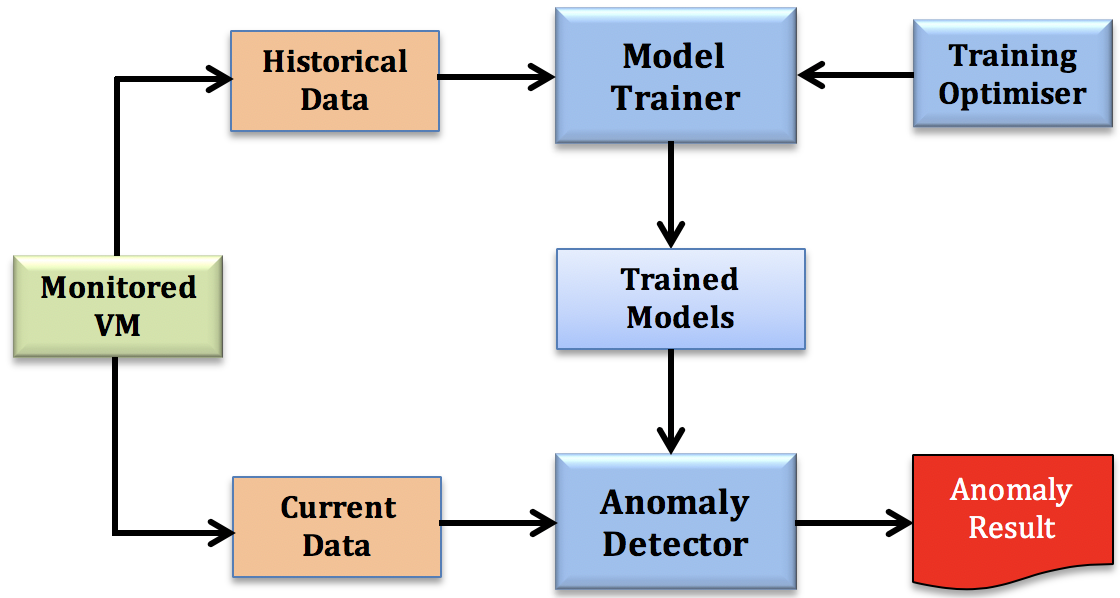
\includegraphics[width=0.7\textwidth]{figures/RADS_Overview}
   \caption{RADS overview}
  \label{fig:overview}
\end{figure}

%\textcolor{red}{Figure~\ref{fig:overview} presents an overview of RADS where we can see how RADS performs the training and the anomaly detection. 
Figure~\ref{fig:overview} depicts an overview of RADS. 
RADS runs the \textit{Model Trainer} to build or train the OCC models by using the ``positive" samples, i.e. the normal CPU utilisation or the network traffic data, which RADS collects from the hosted VMs in a Cloud data centre. Here it is important to note that RADS collects these training data assuming that the VMs are not affected by any DDoS or cryptomining attack. 
These training data are referred as the historical data as they are stored for a period of time. RADS uses the \textit{Training Optimiser} to decide the optimal amount of historical data to be used for the training of an OCC model. RADS runs the \textit{Anomaly Detector} to analyse the current data, i.e. the last one minute of CPU utilisation or the network traffic data by using the trained model. The model flags an anomaly whenever a VM's CPU or network usage pattern deviates significantly from its ``normal" pattern that is learned by the model. 
In both the training and the anomaly detection, RADS uses its window-based time series analysis as discussed in the previous section. 

%third phase - TRAINING OPTIMISER
\begin{algorithm}
\caption{Training Optimisation}
\label{raids_algorithm_training_optimiser}
%\algnewcommand\algorithmicheadingA{\underline{\textbf{{Data Pre-processing}}}}
\algnewcommand\algorithmicinput{\textbf{input:}}
\algnewcommand\algorithmicoutput{\textbf{output:}}
\algnewcommand\algorithmicabb{\textbf{abbreviation:}}
%\algnewcommand\HEADINGA{\item[\algorithmicheadingA]}
\algnewcommand\INPUT{\item[\algorithmicinput]}
\algnewcommand\OUTPUT{\item[\algorithmicoutput]}
\algnewcommand\ABB{\item[\algorithmicabb]}

\begin{algorithmic}[1]
%\algnewcommand\algorithmicheadingC{\underline{\textbf{{Intrusion Detection}}}}
%\algnewcommand\HEADINGC{\item[\algorithmicheadingC]}
%\HEADINGC
\INPUT $SPT$ - \textit{Stability Period Threshold}
%number of minutes to check OCC model's performance before declaring the model as stable
 \OUTPUT $TrainingStatus$ - first\_run/running/stopped/completed
 \ABB 
$ADR = Anomaly Detection Results$
\Statex
%\State $ModelStatus = ``stopped'" $
%\State RUN \textbf{Intrusion Detector} (Algorithm~\ref{raids_algorithm_intrusion_detection}) every 1 minute and store intrusion detection results in $IDR\_File$ 
%; IDR - Intrusion Detection Result
\For {\textbf{each} VM $vm_i$ \textbf{where} \textit{i=1,...,N}}
%\State $trainingStartTime=current\_time()$ \Comment time in minutes
\If {$TrainingStatus_i != ``completed"$} %\Comment execute training every 5 minutes 
%\State RUN algorithm \textbf{Training Data Pre-processing} \Comment execute in every 5 minutes 
%\State RUN \textbf{Model Trainer} (Algorithm~\ref{raids_algorithm_model_training}) % every 5 minute
\If {($TrainingStatus_i = ``first\_run"$ OR \textbf{ADR} contains ``anomaly")} 
\State RUN \textbf{Model Trainer}
\State $TrainingStatus_i = ``running"$
\State $stabilityPeriod_i = 0$
\State $break$
\Else 
%\State INCREMENT stabilityPeriod BY 5 minutes 
\State $stabilityPeriod_i = stabilityPeriod_i + 5$
\EndIf
\If {$(stabilityPeriod_i = SPT)$}
\State $TrainingStatus_i = ``completed"$
\Else
\State $TrainingStatus_i = ``stopped"$
\EndIf
\State CLEAR $ADR\_File$
\EndIf
\EndFor
%\State \textbf{return} $ModelStatus$ \newline
%\State \textbf{Store} $ModelStatus$ in  \textbf{Model Storage} \newline
\end{algorithmic}
\end{algorithm}
%\vfill


%third phase - INTRUSION DETECTION
\begin{algorithm}
\caption{Anomaly Detection}
\label{raids_algorithm_intrusion_detection}
%\algnewcommand\algorithmicheadingA{\underline{\textbf{{Data Pre-processing}}}}
\algnewcommand\algorithmicinput{\textbf{input:}}
\algnewcommand\algorithmicoutput{\textbf{output:}}
\algnewcommand\algorithmicabb{\textbf{abbreviation:}}
%\algnewcommand\HEADINGA{\item[\algorithmicheadingA]}
\algnewcommand\INPUT{\item[\algorithmicinput]}
\algnewcommand\OUTPUT{\item[\algorithmicoutput]}
\algnewcommand\ABB{\item[\algorithmicabb]}

\begin{algorithmic}[1]
%\algnewcommand\algorithmicheadingC{\underline{\textbf{{Intrusion Detection}}}}
%\algnewcommand\HEADINGC{\item[\algorithmicheadingC]}
%\HEADINGC
%\INPUT $INN_{testing}$ - N normalised input instances for testing (one for each VM); $M$ - set of N trained OCC models
\INPUT $CurrentData$ - last one minute of CPU utilisation or network traffic data for each VM; $M$ - set of trained OCC models (one for each VM)
%\OUTPUT $INN_{testing}$ - normalised input instance for testing ; total N instances for N Cloud applications
 \OUTPUT $ADR$ - Anomaly Detection Result (one for each VM)
\Statex
\For {\textbf{each} VM $vm_i$ \textbf{where} \textit{i=1,...,N}}
\State $classificationResult_i=M_i.classify(CurrentData_i)$
 \If {$(classificationResult_i = ``positive")$}
\State $ADR_i= ``normal"$
\Else %If {($classificaitonResult_i = 1$)}
\State $ADR_i= ``anomaly"$
\EndIf
\EndFor
%\State \textbf{Store} ADR in \textbf{Detection Results} \newline
%\State \textbf{return} $IDR$ \newline
\end{algorithmic}
\end{algorithm}
%\vfill

\begin{figure*}
  % {\epsfig{file = figures/RAIDS_framework, width = \textwidth, height=4cm}}
  \centering
     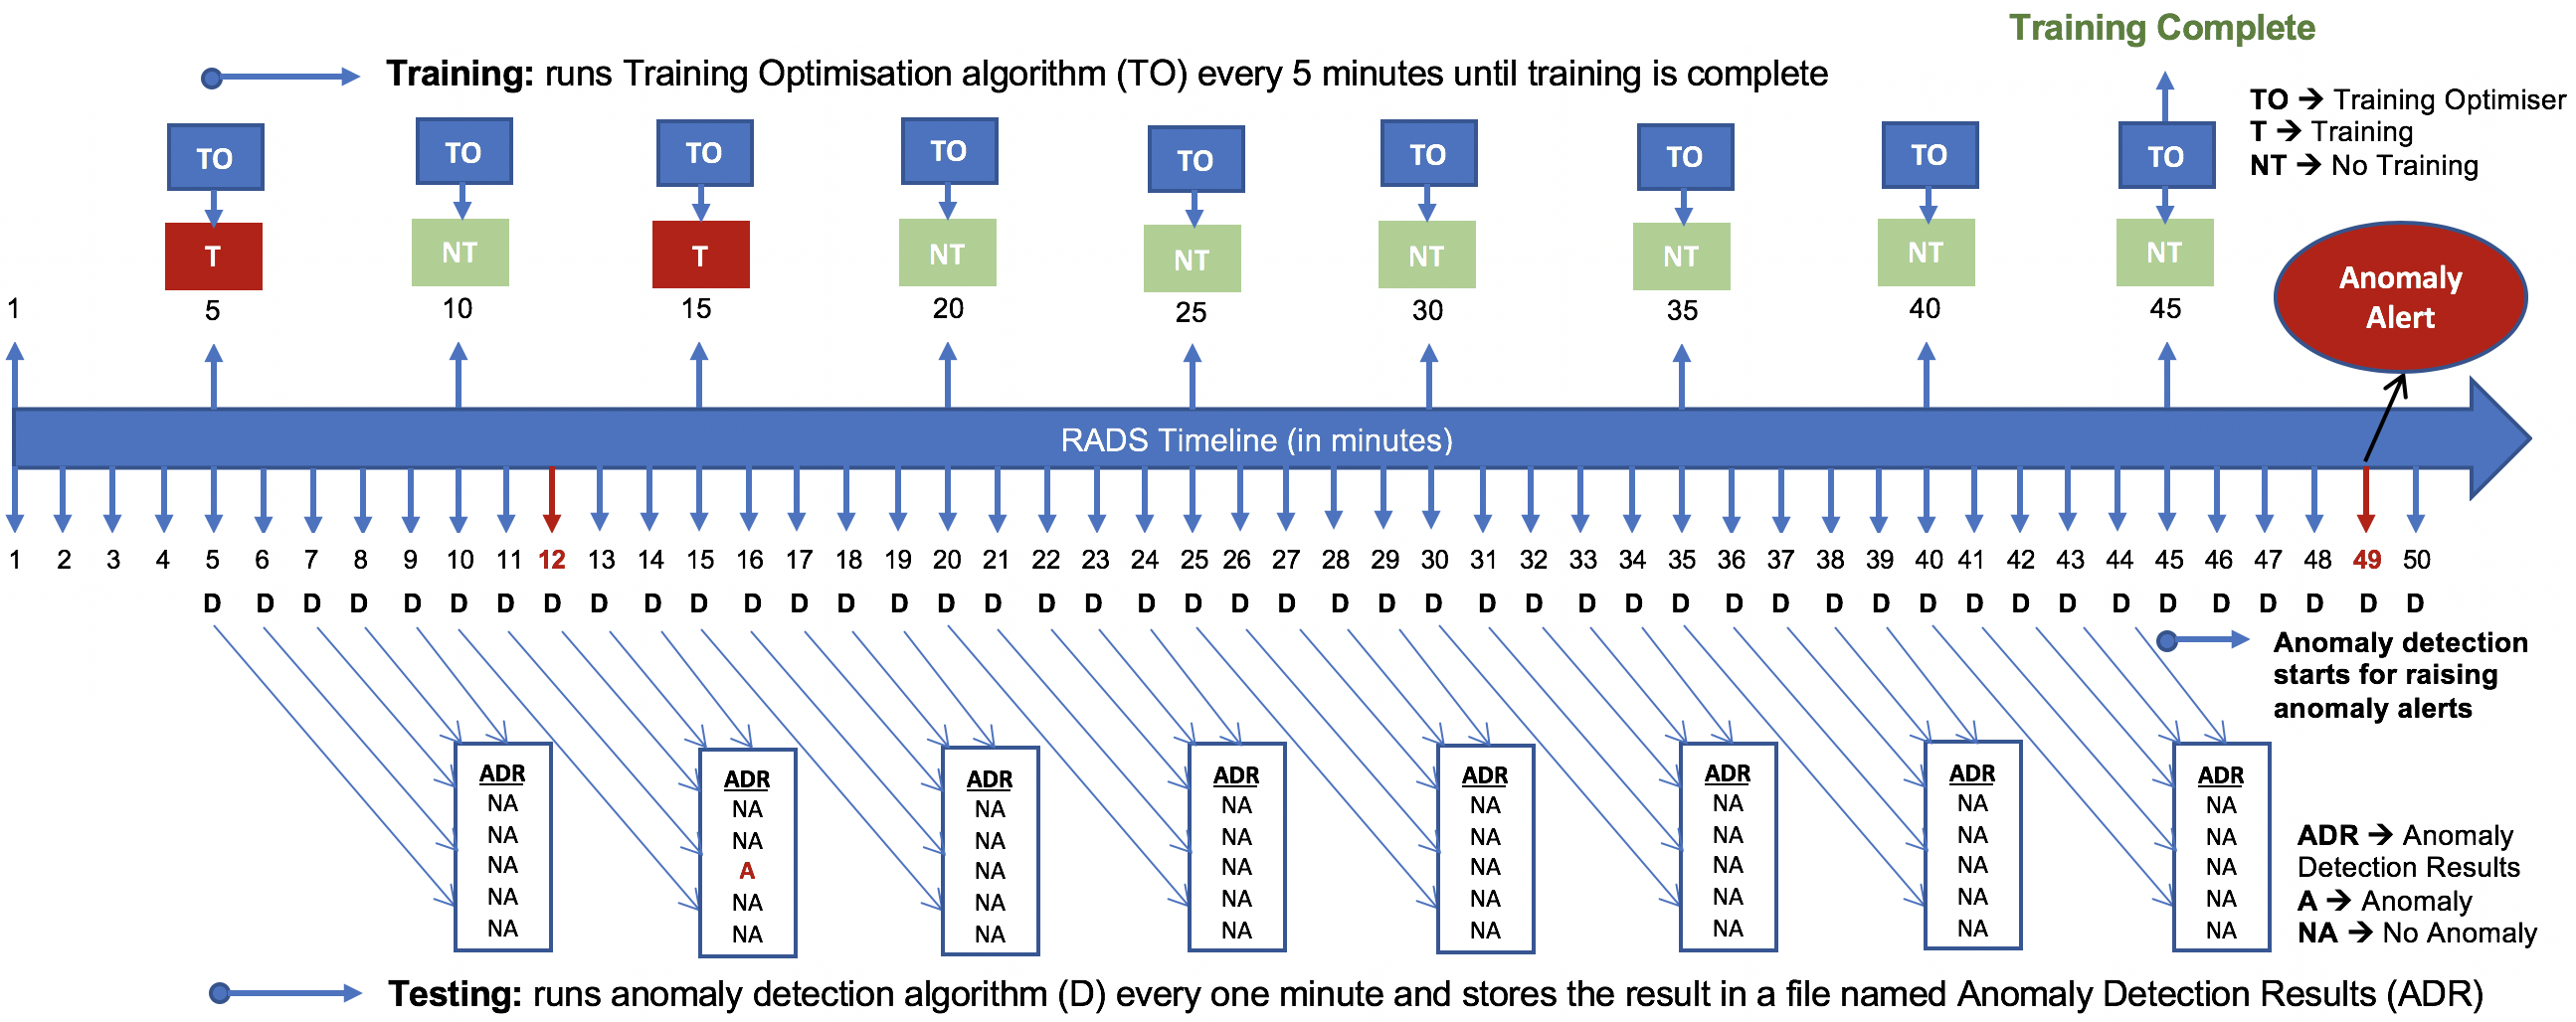
\includegraphics[width=1\textwidth]{figures/RADS_Timeline}
   \caption{RADS  real-time training and anomaly detection}
  \label{fig:timeline}
\end{figure*}
%\vfill

We explain the real-time training and anomaly detection of RADS using a timeline as depicted in Figure~\ref{fig:timeline}. Specifically, we present the timeline of 50 minutes of RADS activity while performing training and detecting anomalies in real-time for a specific VM. We set up the behaviour of the VM artificially where the VM is behaving normally at all times except for minutes 12 and 49 where the VM experiences a genuine spike and an anomaly, respectively. For the first five minutes, RADS remain idle in order to accumulate data points to work with. At the end of 5\textsuperscript{th} minute, RADS starts its training which runs the training optimisation algorithm (TO) (Algorithm~\ref{raids_algorithm_training_optimiser}) every 5 minutes and starts its testing which runs the anomaly detection algorithm (D) (Algorithm~\ref{raids_algorithm_intrusion_detection}) every 1 minute. 
%The time intervals for running TO and D are decided based on our experimental findings. 
When the TO runs for the first time (at the end of 5\textsuperscript{th} minute), it performs the training to build the OCC model for the first time. In the later occasions, the TO evaluates the performance of the trained model by checking whether the model is identifying the VM's behaviour accurately without any false positive. 
This checking is performed by analysing the last five minutes of the anomaly detection results (ADR) obtained from D.
%; the results are stored in a file named Anomaly Detection Results (ADR). 
%This checking is performed by analysing the last five minutes of the results obtained from D; the results are stored in a file named Anomaly Detection Results (ADR). 
We assume that the VM is anomaly-free during the runtime of TO. 
Therefore, if the ADR contains ``anomaly" or ``A", that means that there is an anomaly falsely flagged by the trained model and the model needs to be trained again; in the timeline we can see that at the end of 15\textsuperscript{th} minute the training is performed again due to the occurrence of a false positive generated by the genuine spike at 12\textsuperscript{th} minute.
If the ADR does not contain ``anomaly" or ``A", that means that the model is correctly identifying the VM's behaviour and the model does not need further training; in the timeline we can see that at the end of 10\textsuperscript{th}, 20\textsuperscript{th}, 25\textsuperscript{th}, 30\textsuperscript{th}, 35\textsuperscript{th}, 40\textsuperscript{th}, and 45\textsuperscript{th} minutes the training is stopped. 

The period of time for which the model correctly identifies the ``normal" behaviour, is considered as the stability period for the model. The stability period is incremented with each correct identification by the model (e.g. in the timeline while moving from minute 15 to 45, the stability period is incremented to 30 minutes). Whenever the stability period reaches its threshold value, the TO declares that the training is complete; in the timeline we can see that at the end of 45\textsuperscript{th} minute as we set the threshold value to 30 minutes, which is based on the behaviour of the workloads executed in our testbed. 
However, the threshold for the stability period needs to be adjusted for different VMs based on their workload behaviour; a Cloud data centre may do this based on the type of the instances. 
Once the training is complete, RADS starts its anomaly detection for raising anomaly alerts; in the timeline we can see how RADS raises an anomaly alert at the 49\textsuperscript{th} minute due to the anomalous behaviour of the VM.

%In our experiments, we decided to set the stability period threshold to be 30 minutes, which is based on the behaviour of the workloads executed in our testbed (lab-based Cloud data centre). 
%}
%In both the training and the anomaly detection, RADS uses its window-based time series analysis as discussed in the previous section. }

%The module runs every one minute and stores the detection results in the \textbf{Detection Results}. The storing of the detection results is for the purpose of dynamically deciding the training duration for each OCC model; which allows performing real-time training of the OCC models where the models get updated in real-time at regular intervals until they start performing accurately. 
%To achieve this, RADS applies a heuristic that dynamically decides the training duration for each OCC model.
%As discussed in Section~\ref{sec:introduction}, due to the dynamic nature of Cloud applications, it is required to dynamically decide the training duration for the behavioural models based on the behaviour of the applications. Static models, which are built with fixed training duration may result in low detection accuracy due to model overfitting or underfitting issues.
%The storing of the detection results for a VM continues while the model status for that VM is not ``completed", which means until the model is completely trained for that VM. If the model is completely trained for a VM and an ``anomaly" is detected, RADS flags an anomaly alarm. 


%Finally, we illustrate how RADS dynamically decides the training duration for each OCC model using the \textit{Training Optimiser algorithm} (Algorithm~\ref{raids_algorithm_training_optimiser}).
%This is an important feature of RADS, which can train the OCC models with appropriate set of training data in order to reduce the effect of model overfitting or underfitting. This can also help in dealing with the behavioural changes in workload over time (referred to as concept drift).
%one important feature of the \textbf{Model Trainer} module, which is its ability to dynamically decide the training duration. This feature helps to train the OCC models with appropriate set of training data to reduce the effect of model overfitting or underfitting. 
%As discussed in Section~\ref{sec:introduction}, due to the dynamic nature of Cloud applications, it is required to dynamically decide the training duration for the behavioural models based on the behaviour of the applications. Static models, which are built with fixed training duration may result in low detection accuracy due to model overfitting or underfitting issues.
%The algorithm runs every five minutes and decides whether the training of the OCC model for a particular VM needs to be run or stopped. This decision is based on the real-time performance of the models, which is evaluated by checking whether the model for a VM is identifying the VM's ``normal" resource usage pattern accurately without any false positive for a significant period of time. This checking is performed by analysing the last five minutes of the anomaly detection results (ADR) for that VM. If the ADR contain ``anomaly", that means that there is an anomaly falsely flagged by the trained model and the model for the VM needs to be trained again. Hence, the model training continues for that VM. If the ADR do not contain ``anomaly", that means that the model is correctly identifying the VM's ``normal" resource usage pattern and the model does not need further training. The period of time for which the model correctly identifies the ``normal" usage pattern, is considered as the stability period for the model. The stability period is incremented with each correct identification by the model. Whenever the stability period for a particular model reaches the threshold value set for the stability period, the module declares that the training is complete for that model and updates the model status as ``completed". The threshold for the stability period needs to be decided based on the VMs' workload behaviour; a Cloud data centre may take this decision based on the type of the instances. In our experiments, we decided to set the stability period threshold to be 30 minutes, which is based on the behaviour of the workloads executed in our testbed (lab-based Cloud data centre). 
%We present the algorithm designed for dynamically deciding the training duration in Algorithm~\ref{raids_algorithm_training_optimiser}.


\section{RADS Framework}
\label{sec:framework} 

\begin{figure*}
  % {\epsfig{file = figures/RAIDS_framework, width = \textwidth, height=4cm}}
  \centering
     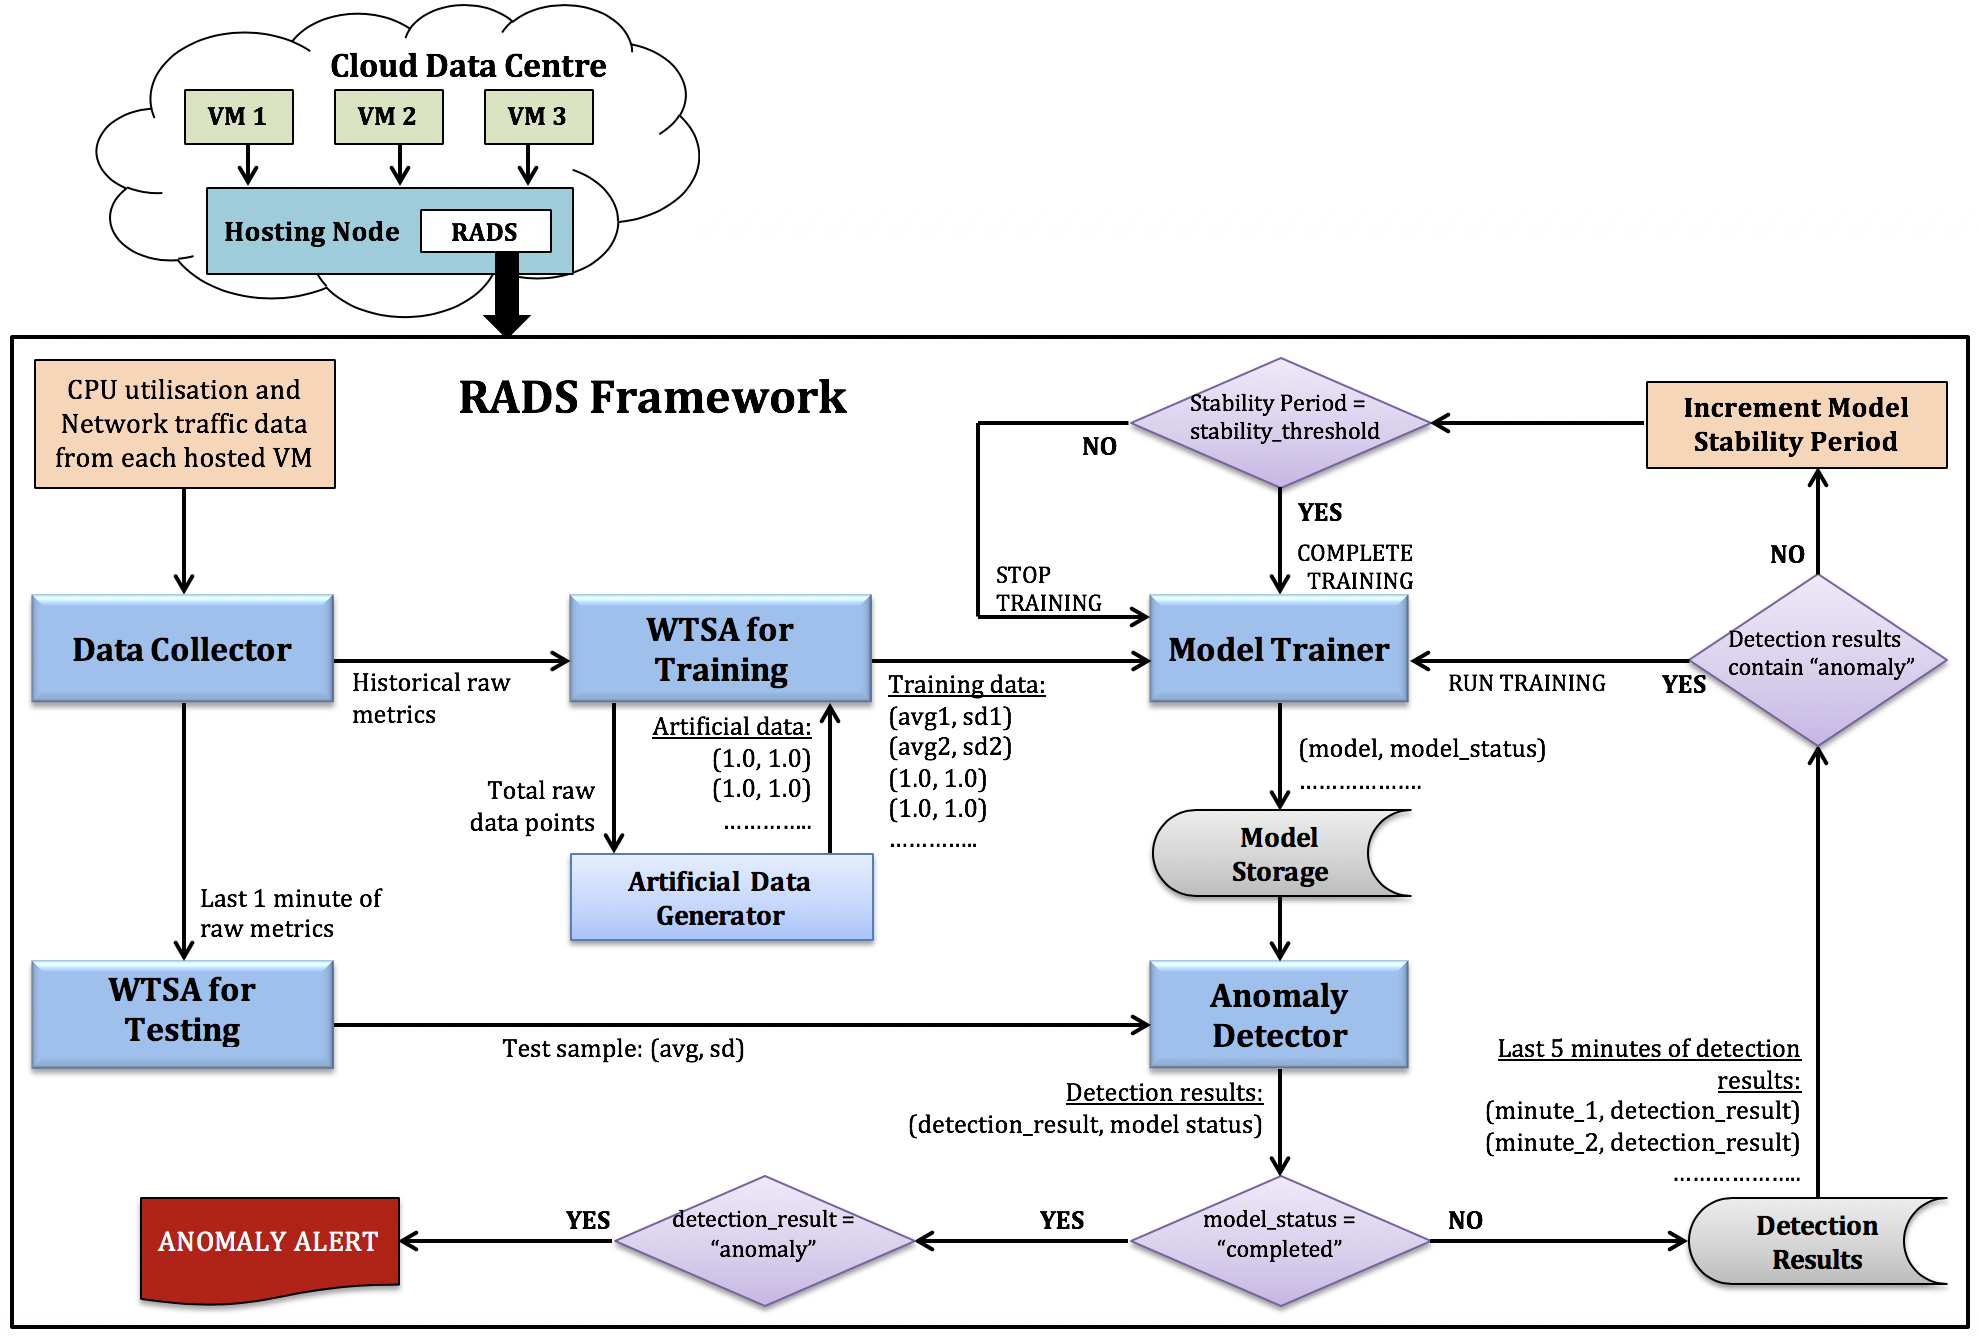
\includegraphics[width=0.9\textwidth]{figures/RADS_Framework}
   \caption{RADS framework}
  \label{fig:framework}
\end{figure*}
%\vfill

\noindent In this section we present the detailed framework of RADS. 
Figure~\ref{fig:framework} depicts the framework, which is designed to be implemented on each hosting node in a Cloud data centre locally, where it can monitor all the hosted VMs in order to detect the VM-level anomalies. % in their resource usage.
%Importantly, all the operations of RADS are in real-time in order to detect the anomalies as they appear.

\subsection{Data Collection}
\noindent RADS uses the \textit{Data Collector} module to collect the CPU utilisation and the network traffic (total size of network packets transmitted and received) metrics of each of the hosted VMs. The frequency of collecting these metrics is 5 seconds which allows capture of the CPU and network usage behaviour in a fine-grained manner.
The module runs virt-top\footnote{http://people.redhat.com/rjones/virt-top/} (a top-like utility for retrieving statistics of virtualised domains) on the hosting node for collecting the VM-level metrics. 
%\subsection{Window-based Time Series Analysis for Training}
%RADS processes the raw metrics before they are used as the training data for training the OCC models or as the test sample for detecting anomaly. RADSs uses two modules for this purpose: \textbf{Data Pre-processor for Training} which processes the historical raw metrics to prepare them as the training data and \textbf{Data Pre-processor for Testing} which processes the last one minute of raw metrics to prepare them as test sample. The modules consider window-based processing of the raw metrics.


%PRE-PROCESSING FOR TRAINING
%\vfill
\begin{algorithm}
\caption{Window-based Time Series Analysis (WTSA) For Training}
\label{raids_algorithm_pre-processing_1}
%\algnewcommand\algorithmicheadingA{\underline{\textbf{{Data Pre-processing}}}}
\algnewcommand\algorithmicinput{\textbf{input:}}
\algnewcommand\algorithmicoutput{\textbf{output:}}
\algnewcommand\algorithmicabb{\textbf{abbreviation:}}
%\algnewcommand\HEADINGA{\item[\algorithmicheadingA]}
\algnewcommand\INPUT{\item[\algorithmicinput]}
\algnewcommand\OUTPUT{\item[\algorithmicoutput]}
\algnewcommand\ABB{\item[\algorithmicabb]}

\begin{algorithmic}[1]
%\algnewcommand\algorithmicheadingAA{\underline{\textbf{{(a) Training Data Pre-processing}}}}
%\algnewcommand\HEADINGAA{\item[\algorithmicheadingAA]}
%\HEADINGAA
\INPUT $Raw_{historical}$ - historical raw metrics of N VMs; $DW$ - distribution window = 1 minute
\OUTPUT $INN_{training}$ - set of normalised input instances for training; total N sets for N VMs
%\OUTPUT $V_{training}$ - set of vectors as training data; total N sets for N VMs.
\ABB 
$avg = Average$; $sd = Standard Deviation$
\Statex
\For {\textbf{each} VM $vm_i$ \textbf{where} \textit{i=1,...,N}}
\State $dataBin(DB_{ij}) = Raw_{historical_i} / DW$ \thinspace \thinspace \thinspace \thinspace \textbf{where} \textit{j=1,...,B (total number of bins)}
\State $inputInstances(IN_i)=initiate()$
\For {\textbf{each} $DB_{ij}$}
\State $avg=DB_{ij}.getAvg()$
\State $sd=DB_{ij}.getSD()$
\State $inputInstance(in_j)=\big[avg, sd\big]$
\State $IN_i.addInstance(in_j)$
\State $IN_i.addClassLabel(``positive")$
\EndFor
\State $INN_{training_i} = IN_i.normalise() $ 
\For {\textbf{each} $DB_{ij}$}
\State $artificialInstance(art_j)=\big[1.0, 1.0\big]$ %\Comment {Mean = 1.0, SD = 1.0; the maximum of normalised values to artificially build up the third class of data to capture spike behaviour}
\State $INN_{training_i}.addInstance(art_j)$
\State $INN_{training_i}.addClassLabel(``positive")$
\EndFor 
%\State $inputInstancesNormalised(INN_{training_i}) = IN_i.normalise() $ 
%\Comment {all normalised values are in the range 0-1}
\EndFor
%\For {\textbf{each} $INN_{training_i}$}
%\State $artificialInstance(art_j)=\big[1.0, 1.0\big]$ %\Comment {Mean = 1.0, SD = 1.0; the maximum of normalised values to artificially build up the third class of data to capture spike behaviour}
%\State $INN_{training_i}.addInstance(art_j)$
%\State $INN_{training_i}.addClassLabel(``positive")$
%\EndFor 
\State \textbf{return} $INN_{training}$ \newline
\end{algorithmic}
\end{algorithm}

\subsection{Window-based Time Series Analysis (WTSA) For Training}
\noindent For each of the hosted VMs, the \textit{WTSA for Training} first takes all the historical raw metrics and distributes them into a number of data bins with equal window size of 1 minute, and second calculates the average (avg) and the standard deviation (sd) of the metrics in each bin. Thus, from each data bin, the module produces a vector: (avg, sd). 
%As mentioned earlier, we selected the window size to be 1 minute as we experimentally found that anything shorter than this does not help in reducing the noise or spikes from the resource utilisation and anything longer than this does not capture the short-term utilisation behaviour.
%The algorithm normalises the instances generated from the data bins (pseudocode line 12). Normalisation helps to improve the classification results as we consider the metrics (CPU utilisation and network traffic) which have different units. The normalisation is performed by using Equation 2.
In addition, the module generates artificial data points which represent the genuine workload spikes (see Section~\ref{sec:approach}). 
%Taking the decision on how many artificial data points to use is a challenging task as on the one hand, using small number of artificial data points may become ineffective and on the other hand, using large number of artificial data points may result in classification model overfitting and increase computation time and resource usage.  
The number of artificial data points is equal to the total number of raw data points, which we have decided after evaluating the performance of RADS with varying number of artificial data points.
%This is supported by the experimental findings in Section~\ref{sec:offline_analysis}.
We represent each artificial data point as a vector: (1.0,1.0) which represents the maximum average and the maximum standard deviation values of the raw metrics as we consider the normalised values of the raw metrics. The normalisation is performed by using Equation~\ref{normalisation}. 
Finally, the module produces a series of vectors for use as training data by combining the vectors which are generated by performing the window-based processing of the raw metrics and the vectors which are generated artificially. 
We present the algorithm for this module in Algorithm~\ref{raids_algorithm_pre-processing_1}.

\subsection{Window-based Time Series Analysis (WTSA) For Testing}
\noindent The \textit{WTSA For Testing} module takes only the last one minute of raw metrics and calculates the average (avg) and the standard deviation (sd) of these metrics to produce the vector (avg, sd). This vector is considered as the test sample for detecting an anomaly. We present the algorithm for this module in Algorithm~\ref{raids_algorithm_pre-processing_2}. The algorithm normalises the \textit{avg} and \textit{sd} values before they are combined as a vector, as defined in Equation~\ref{normalisation}. Importantly, this normalisation is performed against the training data, where minimum and the maximum values are taken from the training data set. 
%This is necessary in order to use the test sample as input to the OCC models which are trained by the training data.
This is necessary in order to achieve the same normalisation for both the training and the testing data.
%In addition to preparing the test sample, this algorithm also verifies whether the test sample represents genuine workload spikes or not. 
%This is based on the following observation from Section~\ref{sec:problem_definition}: \textit{average value of raw data measured during the workload spike situation is higher than the average values measured during the normal situation, which is accompanied by a very high standard deviation value (higher than the standard deviation values measured during the normal and the anomalous situations).}
%The algorithm checks if the normalised avg and sd values are greater than 1.0 (pseudocode lines 5-9), i.e. if they are greater than the maximum average and standard deviation values observed in the training data set. If this check returns true then both the normalised avg and sd values are set to 1.0 and thus, the test sample becomes: (1.0,1.0). This helps the OCC models to identify the test sample representing genuine workload spikes as ``normal" as the model training data include artificial data points: (1.0,1.0), which are labelled as ``positive" or ``normal''. 


\subsection{Model Training}
\noindent RADS builds an OCC model for each hosted VM using the \textit{Model Trainer} module. The OCC models take the training data samples (generated by the \textit{WTSA for Training} module) as the input and learn the ``normal" CPU or network usage pattern of the VMs. 
%These learned OCC models are capable of identifying the deviation in the ``normal" CPU and network usage pattern, which are defined as ``anomalies".
%Thus, the OCC models built for a particular Cloud application is capable of classifying the deviation in the pattern of the application's ``normal" behaviour as ``anomaly" which is occurring due to an intrusion. 
The module stores the OCC models in the \textit{Model Storage}. 
%We present the algorithm designed for this module in Algorithm~\ref{raids_algorithm_model_training}.

\subsection{Anomaly Detection}
\noindent RADS detects the anomalies using the \textit{Anomaly Detector} module. For each VM, the module takes as input the test sample (generated by the \textit{WTSA for Testing} module) and the stored OCC model built for that VM. The module flags an ``anomaly" when there is a deviation in the VM's CPU or network usage pattern. 
%For each identification of anomaly, the module produces ``anomaly" as the detection result. 
%We present the algorithm for this module in Algorithm~\ref{raids_algorithm_intrusion_detection}.

We implemented the RADS modules using Java programming, which imports Apache Common Maths\footnote{http://commons.apache.org/proper/commons-math/} and Weka\footnote{http://www.cs.waikato.ac.nz/ml/weka/} libraries for performing statistical operations and One Class Classification (OCC). 


%PRE-PROCESSING FOR TESTING
\begin{algorithm}
\caption{Window-based Time Series Analysis (WTSA) For Testing}
\label{raids_algorithm_pre-processing_2}
%\algnewcommand\algorithmicheadingA{\underline{\textbf{{Data Pre-processing}}}}
\algnewcommand\algorithmicinput{\textbf{input:}}
\algnewcommand\algorithmicoutput{\textbf{output:}}
\algnewcommand\algorithmicabb{\textbf{abbreviation:}}
%\algnewcommand\HEADINGA{\item[\algorithmicheadingA]}
\algnewcommand\INPUT{\item[\algorithmicinput]}
\algnewcommand\OUTPUT{\item[\algorithmicoutput]}
\algnewcommand\ABB{\item[\algorithmicabb]}

\begin{algorithmic}[1]
%\algnewcommand\algorithmicheadingAB{\underline{\textbf{{(b) Testing Data Pre-processing }}}}
%\algnewcommand\HEADINGAB{\item[\algorithmicheadingAB]}
%\HEADINGAB
\INPUT $Raw_{current}$ - last one minute of raw metrics of N VMs
\OUTPUT $INN_{testing}$ - normalised input instances for testing; total N instances for N VMs
\ABB 
$avg = Average$; $sd = Standard Deviation$
\Statex
\For {\textbf{each} VM $vm_i$ \textbf{where} \textit{i=1,...,N}}
%\State $dataBin(DB_{ij}) = D_i / DW$ \thinspace \thinspace \thinspace \thinspace \textbf{where} \textit{j=1,...,B (total number of bins)}
\State $inputInstances(IN_i)=initiate()$
%\For {\textbf{each} $D_{testing_i}$}
\State $avg_{normalised}=Raw_{current_i}.getAvg().normalise() $
\State $sd_{normalised}=Raw_{current_i}.getSD().normalise() $
\If {$ (avg_{normalised} > 1.0)$ AND $(sd_{normalised} > 1.0)$}
%\State $normalised_avg= 1.0$, $normalised_sd = 1.0$
\State $inputInstance(in)=\big[1.0,1.0\big]$
%\State $IN_i.addInstance(in)$
%\State $INN_{testing_i} = IN_i $ 
%\State $INN_{testing_i} = IN_i $ 
\Else
\State $inputInstance(in)=\big[avg_{normalised}, sd_{normalised}\big]$
\EndIf
\State $IN_i.addInstance(in)$
\State $INN_{testing_i} = IN_i $ 
%\State $INN_{testing_i} = IN_i.normalise() $ 
%\EndIf
%\State $inputInstancesNormalised(INN_{testing_i}) = IN_i.normalise() $ 
%\Comment {all normalised values are in the range 0-1}
%\State $IN_{testing_i}.addClassLabel("positive")$
%\EndFor
%\EndFor 
%\For {\textbf{each} $INN_{testing_i}$}
%\If {$(INN_{testing_i}.getAttribute(avg) > 1.0)$ AND $INN_{testing_i}.getAttribute(sd) > 1.0)$}
%\State $INN_{testing_i}.setAttribute(avg) = 1.0$
%\State $INN_{testing_i}.setAttribute(sd) = 1.0$
%\EndIf
\EndFor
\State \textbf{return} $INN_{testing}$ \newline
\end{algorithmic}
\end{algorithm}

%second phase - MODEL TRAINING
%\begin{algorithm}
%\caption{Model Training}
%\label{raids_algorithm_model_training}
%%\algnewcommand\algorithmicheadingA{\underline{\textbf{{Data Pre-processing}}}}
%\algnewcommand\algorithmicinput{\textbf{input:}}
%\algnewcommand\algorithmicoutput{\textbf{output:}}
%\algnewcommand\algorithmicabb{\textbf{abbreviation:}}
%%\algnewcommand\HEADINGA{\item[\algorithmicheadingA]}
%\algnewcommand\INPUT{\item[\algorithmicinput]}
%\algnewcommand\OUTPUT{\item[\algorithmicoutput]}
%\algnewcommand\ABB{\item[\algorithmicabb]}
%
%\begin{algorithmic}[1]
%%\algnewcommand\algorithmicheadingB{\underline{\textbf{{Model Training}}}}
%%\algnewcommand\HEADINGB{\item[\algorithmicheadingB]}
%%\HEADINGB 
%%\INPUT \textit{A -} arrays of B (total data bins) vectors generated by pre-processing phase; total N arrays for N cloud applications
%%\INPUT $INN_{training}$ - set of normalised input instances for training; total N sets for N cloud applications
%\INPUT $INN_{training}$ - set of normalised input instances for training; total N sets for N VMs
%% $TRR$ - target rejection rate = 0.001
%\OUTPUT $M$ - set of N trained OCC models (one for each VM)
%\Statex
%\For {\textbf{each} VM $vm_i$ \textbf{where} \textit{i=1,...,N}}
%%\State $INN_i.setTargetClassLabel(``positive")$
%%\State $INN_i.setTargetRejectionRate($TRR$ )$ %\Comment {we consider $rejection\_rate = 0.001$ in our experiments}
%\State $M_i=buildOCCModel(INN_{training_i})$
%\EndFor 
%%\State \textbf{return} $M$ \newline
%\State \textbf{Store} $M$ in \textbf{Model Storage} \newline
%\end{algorithmic}
%\end{algorithm}



\section{Evaluation}
\label{sec:experiments}
%\todo[author=DSN,inline]{Have you described the architecture and hardware of the lab-based cloud data centre elsewhere in the paper? What processors, memories, storage, networking, etc you have on the machines?}
%\noindent We performed a number of experiments in a lab-based cloud data centre in order to evaluate the performance of our approach and support the assumption that we discussed in Section~\ref{sec:approach}. In this section we present the results from these experiments and discuss them. Specifically, in this section we attempt to answer the research questions as listed in section~\ref{sec:research-questions}. In section~\ref{sec:experimental_setup} we explain the experimental set-up or testbed set-up that is used to perform the experiments. 
\noindent We performed a number of experiments to evaluate the performance of RADS. The experiments can be classified into: lab-based and real-world. The lab-based experiments were performed in an OpenStack\footnote{https://www.openstack.org} based Cloud data centre, which hosted two representative Cloud applications drawn from the CloudSuite\footnote{http://cloudsuite.ch} benchmark suite. The real-world experiments were carried out on the real-world workload traces~\cite{workloadCCGRID:2015} collected from a Cloud data centre named Bitbrains\footnote{https://www.solvinity.com}.
In this section we present the results from these experiments and discuss them. 
Specifically, we attempt to answer the following research questions: 
%Specifically, in this section we attempt to answer the research questions listed in section~\ref{sec:research-questions}. 
%In section~\ref{sec:experimental_setup} we explain the experimental set-up or testbed set-up that is used to perform the real-time experiments. 
%Section~\ref{sec:behavioural_analysis} presents the behavioural pattern analysis of various cloud applications under both normal and security attack conditions. Finally, we evaluate the effectiveness and efficiency of RAIDS in Section~\ref{sec:raids-performance} and section~\ref{sec:raids-efficiency} respectively. 
%\subsection{Research Questions}
%\label{sec:research-questions}
%\noindent The evaluation process aims to answer the following research questions:
\begin{enumerate}[{(1)}]
%\item Do the experimental results obtained from running various cloud applications verify the problems identified (in Section~\ref{sec:problem_definition}) in the existing statistical approaches used for IDSs. 
%\item Does the experimental evidence support our \textbf{assumption} that we made in Section~\ref{sec:approach}?
	%\todo[author=DSN,inline]{You need to restate this assumption here, the reader may not be able to remember everything!}
%\item Does using a combination of the average and the standard deviation of the raw data solves the problems identified in Section~\ref{sec:problem_definition}?
%Does using a combination of the average and the standard deviation of the raw data solves this problem?}
%\item Are there cases when the state-of-the-art average and entropy based techniques fail in successfully differentiating between cloud applications' normal behavioural pattern that may carry instantaneous spikes and anomalous behavioural pattern that arise due to the security attacks? Does using a combination of the average and the standard deviation of the raw data solves this problem?
%\item What is the accuracy of RAIDS while it uses a combination of average and standard deviation of the raw data as the data pre-processing approach? Does this accuracy outperform the accuracy that is achieved by using state-of-the art average and entropy based approaches?
%\item What is the performance of RAIDS in detecting Cloud intru- sions in real-time? Does RAIDS achieves better performance while using the proposed data pre-processing approach which is based on the average and the standard deviation than that achieved when using state-of-the-art data pre-processing approaches for Cloud IDSs which are based on either the average or the entropy?
\item Can RADS accurately detect Cloud anomalies occurring due to DDoS and cryptomining attacks in real-time? 
\item Can RADS window-based time series analysis outperform the state-of-the-art average and entropy based analyses in terms of accuracy and false positive rate? 
%\item Does the proposed data pre-processing approach which is based on the average and the standard deviation achieves better performance compared to the state-of-the-art data pre-processing approaches for Cloud IDSs which are based on either the average or the entropy? 
%\item While operating in real-time, how much overhead does RAIDS impose on the hosting node resources and how long does RAIDS take to complete the training and the intrusion detection process? 
\item Can RADS be used as a lightweight tool in terms of consuming minimal computing resources and processing time in a Cloud data centre? %used as a lightweight tool for detecting Cloud anomalies in real-time  operating in real-time, how much overhead does RAIDS impose on the hosting node resources and how long does RAIDS take to complete the training and the intrusion detection process? 
%\item What is the performance of RAIDS in terms of dealing with the genuine workload spikes observed in the real-world Cloud data centre workload traces? 
%\item What is the performance of RAIDS in terms of dealing with the genuine workload spikes observed in the real-world Cloud data centre workload traces? 
%\item \textcolor{red}{How RADS responses towards genuine workload spikes observed in a real-world Cloud data centre? 
\item Does RADS maintain its performance in terms of removing false positives while analysing real-world Cloud workload traces?
%Does RAIDS correctly classify such spikes as ``normal" or does it flag them as "anomaly" and raise false alarms? 
%Does RAIDS raise fewer false positives while using its data pre-processing approach than when using state-of-the-art data pre-processing approaches (based on either average or entropy)?
\end{enumerate}

%\subsection{Evaluation of RAIDS in a Lab-based Cloud Data Centre}
\subsection{Lab-based Experiments}
\label{sec:realtime_analysis}
%\noindent In this section we evaluate the performance of RADS in detecting DDoS and cryptomining attacks while running two representative Cloud applications (Graph Analytics and Media Streaming) in our lab-based Cloud data centre. Also, we evaluate the efficiency of RAIDS in terms of the system resources that it consumes and the time it takes while performing real-time training of the classification models and testing of the new samples to detect the intrusions.
\noindent In this section we evaluate the performance of RADS in detecting DDoS and cryptomining attacks in our lab-based Cloud data centre. Also, we evaluate the efficiency of RADS in terms of the system resources that it consumes and the time it takes while performing real-time training of the classification models and testing of new samples to detect the anomalies.
%The evaluation includes results under different data pre-processing approaches. 
In particular, in this section we attempt to answer research questions 1, 2, and 3.
%\noindent In this section we evaluate the effectiveness of RAIDS in detecting the emulated security attacks: DDoS and backdoor channel attacks while running the cloud applications (Graph Analytics and Media Streaming) in our testbed. The evaluation includes results under different data pre-processing approaches. In particular, in this section we attempt to answer the research question 4.

%\subsubsection{Testbed}
%\label{sec:testbed}
%\noindent 
\textbf{Testbed:} Our testbed is an OpenStack based Cloud data centre which consists of four compute nodes. Each compute node is a Dell PowerEdge R420 server that runs CentOS 6.6 and has 24 cores, 2-way hyper-threaded, clocked at 2.20 GHz with 12GB DRAM clocked at 1600 MHz. The nodes include two 7.2K RPM hard drives with 1TB of SATA in RAID 0 and a single 1GBE port. KVM is the default hypervisor of the nodes. 

%\subsubsection{Experimental Set-up}
%\label{sec:experimental_setup}
%\noindent In this section we describe the experimental set-up. 
%\subsubsection{Experimental Set-up for Real-time Experiment}
%\textit{Testbed}: We set up the experiments in an OpenStack based Cloud data centre (testbed). The testbed includes four compute nodes each of which is a Dell PowerEdge R420 server. Each of the compute nodes runs CentOS 6.6 and has 24 cores, 2-way hyper-threaded, clocked at 2.20 GHz with 12GB DRAM clocked at 1600 MHz. The nodes include two 7.2K RPM hard drives with 1TB of SATA in RAID 0 and a single 1GBE port. KVM is the default hypervisor of the nodes. 
%In order to examine the Cloud application behaviour with and without security attacks or workload spikes, we executed two Cloud applications (Graph Analytics and Media Streaming) from the CloudSuite workload collection. The experimental set-up for Graph Analytics application is depicted in Figure~\ref{fig:testbed_analytics} and the experimental set-up for Media Streaming application is depicted in Figure~\ref{fig:testbed_media}.
%\noindent 
\textbf{Experimental Set-up:} We hosted two Cloud applications in our testbed: Graph Analytics (representing CPU intensive Cloud applications) and Media Streaming (representing network intensive Cloud applications). The experimental set-up for the Graph Analytics is depicted in Figure~\ref{fig:testbed_analytics} and the experimental set-up for the Media Streaming is depicted in Figure~\ref{fig:testbed_media}.
The Graph Analytics application performs PageRank on a Twitter dataset using the Spark\footnote{http://spark.apache.org} framework. We deployed the application on a dedicated ``Analytics VM" with the configuration: 8GB of RAM and 4 cores of CPU. Under ``normal" conditions we executed the application using only 1 core of CPU.
The Media Streaming application runs a streaming server using the Nginx\footnote{https://github.com/nginx/nginxweb} server, which hosts videos of various lengths and qualities.  
The clients send requests to the hosted videos to create realistic media streaming behaviour.  
We deployed the server on a dedicated ``Server VM" with the configuration: 4GB of RAM and 4 cores of CPU and the clients on a dedicated ``Client VM" with the same configuration.
In our experiment, we portrayed ``normal" media streaming behaviour by running 50 clients in the ``Client VM" with ``ShortHi" configuration which requests videos with high bandwidth of 790 Kbps.

% EXPERIMENTAL SET UP / TESTBED FOR GRAPH ANALYTICS
%\vfill
\begin{figure}[!h]
  \vspace{-0.2cm}
  \centering
   {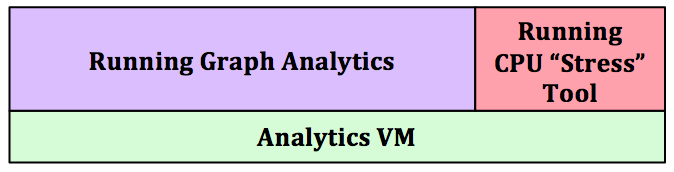
\epsfig{file = figures/RAIDS_testbed_analytics_png, width = 0.5\columnwidth}}
  % \caption{RADS testbed for examining CloudSuite Graph Analytics application behaviour under backdoor channel attack and spike affect}
      \caption{Experimental set-up for Graph Analytics application}
  \label{fig:testbed_analytics}
  \vspace{-0.1cm}
\end{figure}
%\vfill

% EXPERIMENTAL SET UP / TESTBED FOR MEDIA STREAMING
%\vfill
\begin{figure}[!h]
  \vspace{-0.2cm}
  \centering
   {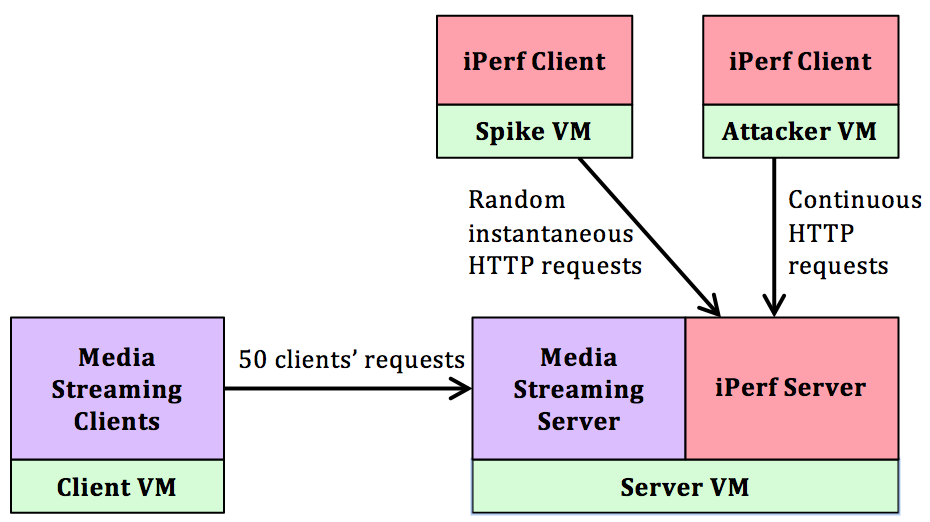
\epsfig{file = figures/RAIDS_testbed_media_png, width = 0.8\columnwidth}}
  % \caption{RAIDS testbed for examining CloudSuite Media Streaming application behaviour under DDoS attack and spike affect}
         \caption{Experimental set-up for Media Streaming application}
  \label{fig:testbed_media}
  \vspace{-0.1cm}
\end{figure}
%\vfill

%\textit{Emulated attacks}: We considered two security attacks in our experiments, which are: backdoor channel attack (for Graph Analytics) and DDoS attack (for Media Streaming). We explained these attacks in detail in Section~\ref{sec:introduction}.
\textit{Emulated attacks}: We emulated the DDoS and the cryptomining attacks targeting the VMs running the Media Streaming server and the Graph Analytics application, respectively. 
%two security attacks in our experiments, which are: backdoor channel attack (for Graph Analytics) and DDoS attack (for Media Streaming). 
Cryptomining attack was emulated by running the ``stress"\footnote{https://people.seas.harvard.edu/\~apw/stress/} tool on the ``Analytics VM" (see Figure~\ref{fig:testbed_analytics}). The ``stress" tool is a simple workload generator, which can impose a configurable amount of CPU, memory, I/O, and disk stress on the system. 
The DDoS attack was emulated by sending continuous HTTP requests from an ``Attacker VM" to the ``Server VM" (see Figure~\ref{fig:testbed_media}) with the help of the iPerf\footnote{https://iperf.fr} tool (``Server VM" as iPerf server and ``Attacker VM" as iPerf client).
%The tool consumes 1/2/3 cores of CPU at different time, which is to produce low-high intensity attacks (low: 1 core, medium: 2 cores, high: 3 cores).
%\todo[author=DSN,inline]{Is this practice of emulating backdoor channel attacks of different intensity by hijacking a different number of cores established? I would think that an attacker would just go for a massive number of VMs (processes, threads,...) to instantiate the attack, without caring too much about how many cores the machine has. Questionmark about methodology here.}
%The DDoS attack is emulated by sending video requests to the Media Streaming server from three different VMs: VM1, VM2, and VM3, which are assumed to be victimised by DDoS attack. Each of these VMs runs 25 clients. They start running the clients at a different time to produce low-high intensity attacks (low: $25$ clients, medium: $25+25$ clients, high: $25+25+25$ clients). 

\textit{Emulated workload spikes}: For the Graph Analytics application, a workload spike was generated by running the ``stress" tool in the ``Analytics VM" for a short period of time (5 seconds). For Media Streaming application, a workload spike was generated by sending HTTP requests for instantaneous period of time (5 seconds) from the ``Attacker VM" to the ``Sever VM" (see Figure~\ref{fig:testbed_media}) with the help of the iPerf tool (``Server VM" as iPerf server and ``Spike VM" as iPerf client).
%\textit{Data Collection}: 
%RAIDS performs both the training of the OCC models and the testing of the test samples for intrusion detection on the hosting node (compute node in case of our test-bed). 
%RADS collected the data required for OCC model training and the anomaly detection by continuously running its \textit{Data Collector} module on the hosting node (compute node in case of our test-bed). 
%RADS \textit{Data Collector} module collected the data required for OCC model training and the anomaly detection by continuously running module on the hosting node (compute node in case of our test-bed). 
%The module stored the data in two different files: (i) \textit{historical\_data\_file}, which stored the historical data required for training and (ii) \textit{current\_data\_file}, which stored the last one minute of data required for testing or anomaly detection. 
%RAIDS \textit{Model Trainer} module performed the training of the OCC models for each Cloud application under examination.  
%RAIDS Training Optimiser algorithm (Algorithm~\ref{raids_algorithm_training_optimiser}) decided the training duration. 
%RAIDS \textit{Intrusion Detector} module tested the test samples and flagged an intrusion whenever it detected an ``anomaly".

%\subsubsection{Experimental Set-up for Offline Experiment}
 %Offline experiments were carried out on the real workload traces [7], which are collected from a Cloud data centre named Bitbrains.

%\subsubsection{Performance Metrics}
\textbf{Performance Metrics:} 
We use a number of standard performance metrics such as precision, recall, accuracy (F1 score), and false positive rate (FPR) to measure the performance of RADS. 
%We use two performance metrics: accuracy (F1 score), and false positive rate (FPR) to measure the performance of RADS. 
%Since RAIDS uses OCC algorithm for identifying the intrusions, all the training data are labelled as "normal". 
RADS reacts with an anomaly alarm whenever it classifies a test sample as ``anomalous", otherwise RADS does not react. 
In our experiments, we declare: (a) False Positives (FP) when RADS raises an alarm but there is no ``anomaly", (b) False Negatives (FN) when RADS fails to raise an alarm but there exists an ``anomaly", (c) True Positives (TP) when RADS raises an alarm and there exists an ``anomaly", (d) True Negatives (TN) when RADS does not raise an alarm and there is no ``anomaly". We define the performance metrics in Equations \ref{eq2}-\ref{eq5}.

% EQUATIONS FOR PERFORMANCE METRICS..
\begin{equation}\label{eq2}
    Precision \quad = \quad   \frac{TP}{TP+FP}
\end{equation}
\begin{equation}\label{eq3}
    Recall \quad = \quad   \frac{TP}{TP+FN}
\end{equation}
\begin{equation}\label{eq4}
    Accuracy (F1 score) \quad = \quad   2\times\frac{Precision \times Recall}{Precision+Recall}
\end{equation}
\begin{equation}\label{eq5}
    FPR \quad = \quad   \frac{FP}{FP+TN}
\end{equation}

Precision gives us the measure of how many of the positive classifications (anomaly alarms) are correct, whereas the recall gives us the measure of RADS's ability to correctly identify an ``anomaly". 
However, precision and recall alone cannot judge the performance of RADS. Therefore, we use Accuracy (F1 score) which gives us the harmonic mean of precision and recall.

%\subsubsection{Training and Testing Data Preparation}
%RAIDS is a real-time IDS where both the training of the classification models and the testing of the new data samples (for intrusion detection) are performed in real-time. RAIDS collected the data for both the training and the testing by continuously running its \textit{data collector} module. The module stored the data in to two different files: (i) \textit{historical\_data\_file}, which stored the historical data required for training and (ii) \textit{current\_data\_file}, which stored the last one minute of data required for testing or intrusion detection. RAIDS training optimiser algorithm decided the amount of historical data required to correctly train the classification models. RAIDS \textit{intrusion detection} module started running only when the classification models were correctly built by RAIDS \textit{model training} module.

% DETECTION RESULTS TABLE

\begin{landscape}

\newcolumntype{L}[1]{>{\raggedright\arraybackslash}p{#1}}
\newcolumntype{C}[1]{>{\centering\arraybackslash}p{#1}}
\newcolumntype{R}[1]{>{\raggedleft\arraybackslash}p{#1}}
\begin{table*}[t]
%\caption{Anomaly detection results of RADS under different data pre-processing approaches}
\caption{Anomaly detection results of RADS under different time series analyses}
\label{tab:test_results} 
\centering
\begin{tabular}{C{2.2cm}C{4.2cm}C{1.7cm}C{1.7cm}C{1.7cm}C{1.5cm}C{1.6cm}} %C{1.5cm}}
  %\hline
  \toprule
  Monitored VM & Time Series Analysis & Training Time (minutes) & \textit{Attack Test} Result & \textit{Spike Test} Result 
  & Accuracy (F1 Score) & False Positive Rate (FPR)\\ %& Overall detection accuracy \\
    \bottomrule
   & & &\begin{tabular}{C{0.5cm}C{0.5cm}}  TP & FN \\  \end{tabular} & \begin{tabular}{C{0.5cm}C{0.5cm}}  FP & TN \\  \end{tabular} \\
    \bottomrule 
        \begin{tabular}{C{2cm}} Graph Analytics VM \\ \end{tabular} 
        & \begin{tabular}{C{4.0cm}} Average \\ Entropy \\ Average \& Std. Deviation \\ \end{tabular} 
        & \begin{tabular}{C{1.2cm}} 45 \\ 105 \\ 130 \end{tabular}
        %& \begin{tabular}{C{1.0cm}} 10 \\  0 \\ 9 \end{tabular}
        %& \begin{tabular}{C{1.0cm}} 10 \\  0 \\ 9 \end{tabular}
         &\begin{tabular}{C{0.5cm}C{0.5cm}} 10 & 0 \\ 0 & 10 \\ 9 & 1 \end{tabular}
         &\begin{tabular}{C{0.5cm}C{0.5cm}} 6 & 24 \\ 2 & 28 \\ 1 & 29 \end{tabular} 
         & \begin{tabular}{C{1.0cm}} 0.77 \\ 0.00 \\ 0.90 \end{tabular}
        & \begin{tabular}{C{1.0cm}} 0.20 \\ 0.07 \\ 0.03 \end{tabular} \\
         %&  \begin{tabular}{C{2.0cm}} 6 \\ 2 \\ 1 \end{tabular} 
         %&  \begin{tabular}{C{2.0cm}} 6 \\ 2 \\ 1 \end{tabular} \\
         

  \hline
    \begin{tabular}{C{2cm}} Media Streaming Server VM \\ \end{tabular} 
       & \begin{tabular}{C{4.0cm}} Average \\ Entropy \\ Average \& Std. Deviation \\  \end{tabular} 
       & \begin{tabular}{C{1.2cm}} 70 \\ 20 \\ 35 \end{tabular}
       %& \begin{tabular}{C{2.0cm}} 10 \\ 10 \\ 9 \end{tabular}
      % & \begin{tabular}{C{2.0cm}} 10 \\ 10 \\ 9 \end{tabular}
      % & \begin{tabular}{C{2.0cm}}  8 \\ 0 \\ 0 \end{tabular}
       &\begin{tabular}{C{0.5cm}C{0.5cm}} 10 & 0 \\ 10 & 0 \\ 9 & 1 \end{tabular}
       &\begin{tabular}{C{0.5cm}C{0.5cm}} 8 & 22 \\ 0 & 30 \\ 0 & 30 \end{tabular} 
        & \begin{tabular}{C{1.0cm}} 0.71 \\ 1.00 \\ 0.95 \end{tabular}
       & \begin{tabular}{C{1.0cm}} 0.27 \\ 0.00 \\ 0.00 \end{tabular} \\
      % & \begin{tabular}{C{2.0cm}}  8 \\ 0 \\ 0 \end{tabular} \\
    \hline
      
\end{tabular}
\end{table*}

\end{landscape}


% END OF DETECTION RESULTS TABLE

%% ACCURACY RESULTS  TABLE
%\newcolumntype{L}[1]{>{\raggedright\arraybackslash}p{#1}}
%\newcolumntype{C}[1]{>{\centering\arraybackslash}p{#1}}
%\newcolumntype{R}[1]{>{\raggedleft\arraybackslash}p{#1}}
%\begin{table*}[t]
%\caption{Effectiveness results of RAIDS under different data pre-processing approaches}
%\label{tab:accuracy_results} 
%\centering
%%\begin{tabular}{|c|c|}
%\begin{tabular}{C{3.0cm}C{4.5cm}C{1.5cm}C{1.5cm}C{1.5cm}C{1.5cm}C{1.7cm}} %C{1.5cm}}
%  \toprule
%  Monitored VM & Data Pre-processing Approach & Number of Observations & Precision & Recall & Accuracy (F1 Score) & False Positive Rate (FPR) \\ %& Overall detection accuracy \\
%    \bottomrule
%        \begin{tabular}{C{2.5cm}} Graph Analytics VM \\ \end{tabular} 
%        & \begin{tabular}{C{4.0cm}} Average \\ Entropy \\ Average \& Standard Deviation \\ \end{tabular} 
%        & \begin{tabular}{C{1.2cm}} 40 \\ 40 \\ 40 \end{tabular} 
%        & \begin{tabular}{C{1.2cm}} 0.63 \\ 0.00 \\ 0.90 \end{tabular}
%         & \begin{tabular}{C{1.2cm}} 1.00 \\ 0.00 \\ 0.90 \end{tabular}
%        & \begin{tabular}{C{1.2cm}} 0.77 \\ 0.00 \\ 0.90 \end{tabular}
%        & \begin{tabular}{C{1.2cm}} 0.20 \\ 0.07 \\ 0.03 \end{tabular} \\
%       
%  \hline
%    \begin{tabular}{C{2.5cm}} Media Streaming Server VM \\ \end{tabular} 
%       & \begin{tabular}{C{4.0cm}} Average \\ Entropy \\ Average \& Standard Deviation \\ \end{tabular} 
%       & \begin{tabular}{C{1.2cm}} 40 \\ 40 \\ 40 \end{tabular}
%       & \begin{tabular}{C{1.2cm}} 0.56 \\ 1.00 \\ 1.00 \end{tabular}
%       & \begin{tabular}{C{1.2cm}} 1.00 \\ 1.00 \\ 0.90 \end{tabular}
%       & \begin{tabular}{C{1.2cm}} 0.71 \\ 1.00 \\ 0.95 \end{tabular}
%       & \begin{tabular}{C{1.2cm}} 0.27 \\ 0.00 \\ 0.00 \end{tabular} \\
%
%    \hline
%      
%\end{tabular}
%\end{table*}
%
% END OF ACCURACY RESULTS TABLE

%\subsubsection{\textbf{Anomaly Detection Performance of RADS}}
\textbf{Anomaly Detection Performance of RADS:}
%To evaluate the anomaly detection performance of RADS we carried out two tests: (i) \textit{Attack Test} which analyses the number of successful anomaly detections by RADS and (ii) \textit{Spike Test} which analyses the number of false positives generated by RADS. 
To evaluate the anomaly detection performance of RADS we carried out two tests: (i) \textit{Attack Test -} during which we emulated the DDoS attack (targeting the VM running the Media Streaming server) or the cryptomining attack (targeting the VM running the Graph Analytics application) continuously for 10 minutes; and (ii) \textit{Spike Test -} during which we emulated workload spikes for 10 times in a random manner in a time period of 30 minutes; there is no emulated attack during this test.
%To measure the accuracy of RAIDS we performed two tests: (i) \textit{intrusion detection test:} to understand RAIDS's successfulness in detecting Cloud security attacks and (ii) \textit{false positive test:} to understand RAIDS's sensitivity towards normal application behaviour. Table~\ref{tab:detection_results} presents the \textit{intrusion detection test} result which shows the number of successful detections by RAIDS, whereas Table~\ref{tab:false_positives} presents \textit{false positive test} result which show the number of false positives generated by RAIDS. The result for the former test is presented for different attack categories under different data pre-processing approaches, similarly the result for the latter test is presented for different spike categories under different data-processing approaches.
During both the tests, we executed the RADS \textit{Anomaly Detector} module on the hosting node. 
%\textit{Model Trainer} and \textit{Anomaly Detector} module 
For both the tests, the module used the same OCC models which were trained by the RADS \textit{Model Trainer} module. 
%Hence, the training times required for different data pre-processing approaches are the same in both the tests. However, the training time is different for different approaches and for different VMs as it is decided by the RADS \textit{Training Optimiser Algorithm} (Algorithm~\ref{raids_algorithm_training_optimiser}).
%During both the tests, we executed RADS \textit{Anomaly Detector} module 
%Both the testing started only after the OCC models were correctly built by RAIDS \textit{Model Trainer} module. 
%The testing time for \textit{Intrusion Detection Test} was 10 minutes, during which we executed each emulated security attack continuously for 10 minutes, whereas the testing time for the \textit{False Positive Test} was 30 minutes, during which we injected the emulated workload spikes for 10 times in random manner. 
%Table~\ref{tab:attack_spike_category} describes both the attack and the spike categories for both cloud applications. 

Table~\ref{tab:test_results} presents the test results under different time series analyses.
From the results we observe 
%the following:
%\begin{enumerate}[{(a)}]
%\item 
that the average based analysis achieves the maximum number of true positives (total 20), but on the other hand, this approach raises the maximum number of false positives (total 14).
%\item 
Entropy raises only 2 false positives in the case of the Graph Analytics VM and no false positives in the case of the Media Streaming server VM, but the problem with the entropy based approach is its poor performance in detecting the attacks (10 false negatives in the case of the Graph Analytics VM).
%\item 
%The proposed data pre-processing approach which uses a combination of the average and the standard deviation, successfully detects the attacks with total 18 true positives. 
RADS window-based time series analysis, which uses a combination of the average and the standard deviation, successfully detects the attacks with total 18 true positives. 
%, which is however less than the average based approach. We have observed that 
We have observed that the false negatives (1 for each of the monitored VMs) arise during the first minute of the \textit{Attack Test}, when the ``anomalous" behaviour due to attack does not occupy the whole 1 minute of the detection window; the time series of the detection window becomes similar to the one depicted in Figure~\ref{fig:one_minute_timeseries}. A test sample generated from such a detection window can be represented as: (high\_average, high\_standard\_deviation), which is wrongly classified as ``normal" by RADS as it considers the short-term ``anomalous" behaviour in the detection window as a genuine workload spike.
%As these false negatives appear only during the first minute of the attack, 
However, these false negatives are trivial due to the fact that they appear only during the first minute of the attack; and DDoS or cryptomining attacks require a considerable amount of time (at least a few minutes) before they become harmful.  
%However, such false negatives do not affect DDoS or cryptomining attack detection as these kind of attacks persist for a long period of time (at least longer than 1 minute) to achieve their goals.
%\item The proposed data pre-processing approach which uses a combination of the average and the standard deviation achieves a good success rate (90\%) in detecting the attacks, which is however less than the average based approach. We have observed that the single time failure of the proposed approach occurs for the first instance of the detection process. During the first minute of the detection process, when the ``anomalous" behaviour due to attack does not occupy the whole 1 minute of the detection window, the timeseries of the detection window becomes similar to the one depicted in Figure~\ref{fig:one_minute_timeseries}. A test sample generated from such a detection window can be represented as: (high\_average, high\_standard\_deviation), which is wrongly classified as ``normal" by RAIDS as it considers that there are genuine workload spikes in the detection window. 
% as a result of obeying the \textbf{assumption} (made in Section~\ref{sec:approach}): \textit{genuine workload spikes during a Cloud application's normal behaviour produce high average values, which are accompanied by very high standard deviation values.}
%We consider the solution of this as future work.
%\end{enumerate}

% ONE MINUTE TIMESERIES
%\vfill
\begin{figure}[!h]
%  \vspace{-0.2cm}
  \centering
      {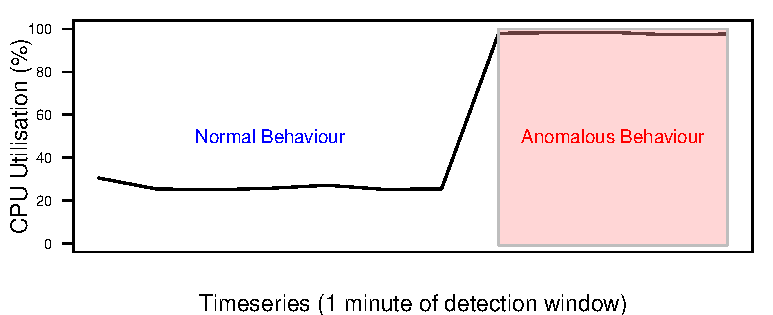
\epsfig{file = figures/one_minute_timeseries, width = 0.8\columnwidth}}
   \caption{The first minute of detection window which includes both the ``normal" and the ``anomalous" behaviour}
  \label{fig:one_minute_timeseries}
 % \vspace{-0.1cm}
\end{figure}
%\vfill

%Therefore, RAIDS wrongly identifies this high value of standard deviation due to security attack as a normal behaviour occurring due to spikes. However, the impact of this depends on the behaviour of the security attack; if the attack establishes gradually i.e. step by step without jumping to high intensity attack straight away, we can expect RAIDS to be able to detect even the first time occurrence of the attack. In any case, we consider this issue to analyse and diagnose further in future.  
		%\todo[author=DSN,inline]{Can you back this argument up with a citation or more experimental evidence?}
%Table~\ref{tab:test_results} further presents the accuracy (F1 score) and the false positive rate (FPR) results of RAIDS under different data pre-processing approaches. In the Table~\ref{tab:accuracy_results}, the number of observations are calculated by adding the number of testing samples in \textit{Intrusion Detection Test} and \textit{False Positive Test}, i.e. ($10+30=40$). All the performance metrics are calculated based on the ``number of successful detections'' and ``false positives'' observed from the two tests (Table~\ref{tab:test_results}).
In order to get a better insight into the anomaly detection performance of RADS, we calculated the accuracy (F1 score) and the false positive rate (FPR) (see Table~\ref{tab:test_results}) using Equations \ref{eq4} and \ref{eq5}, respectively.  
%From the results presented in Table~\ref{tab:accuracy_results} we answer the research question 1 as follows:
These performance metrics answer the research questions 1 and 2 as follows:
\begin{enumerate}[{(a)}]
\item RADS can detect Cloud anomalies occurring due to DDoS and cryptomining attacks in real-time with an accuracy (F1 Score) of 90-95\% and a low false positive rate of 0-3\%.
\item RADS achieves on average 34\% improvement in accuracy and 60\% improvement in false positive rate while using its window-based time series analysis instead of using the state-of-the-art average or entropy based analysis. 
% (based on average and entropy).
%\item Results show that RAIDS achieves 90-95\% accuracy (F1 score) with a low false positive rate of 0-3\% while using the proposed data pre-processing approach which uses the combination of both the average and the standard deviation.
%\item The results further reveal on average 34\% improvement in accuracy and 60\% improvement in false positive rate while using the proposed data pre-processing approach instead of using the state-of-the-art data pre-processing approaches for Cloud IDSs which are based on either the average or the entropy.
%\item Accuracy (F1 score) results show that RAIDS achieves 87-95\% accuracy with a low false positive rate of 0-3\% using its unique data pre-processing approach that uses combination of both the average and the standard deviation.
%\item Accuracy (F1 score) results demonstrate that RAIDS achieves on average 88\% improvement in accuracy and 35\% improvement in false positive rates while using its unique data pre-processing approach instead of using state-of-the-art average or entropy based approaches.
\end{enumerate}
%The anomaly detection performance achieved by RADS in our experiments may vary under different experimental set-up. The performance results discussed above are only indicators of RADS capability in detecting DDoS and cryptomining attacks with high accuracy and low false positive rates.

%\subsubsection{\textbf{Efficiency of RADS}}
\textbf{Efficiency of RADS:}
%In this section we evaluate the efficiency of RAIDS. 
%RAIDS is a real-time IDS and therefore, its important for RAIDS to be efficient in terms of the hosting node resource that it consumes and the time it takes while performing the training of the classification models and the testing of the new samples to detect the intrusions. 
%To evaluate the efficiency of RAIDS we carried out two experiments: (i) \textit{Training Efficiency} which measures the efficiency of RAIDS in training OCC models and (ii) \textit{Testing Efficiency} which measures the efficiency of RAIDS in intrusion detection or testing of the new samples. We performed the experiments on one of the compute nodes in our testbed. 
%The hosting node is a Dell PowerEdge R420 server which runs CentOS 6.6 and has 24 cores, 2-way hyper-threaded, clocked at 2.20 GHz with 24GB DRAM clocked at 1600 MHz. 
%In order to explain the effect of number of hosted VMs on RAIDS efficiency, we carried out the experiments while scaling up the number of VMs from 2 to 10 in the compute node. Although such scaling of VMs does not represent a real Cloud data centre, we attempt to extract out some information on RAIDS efficiency under VM scaled up situations. 
%Also, important to note that, for experimental purpose, we stopped RAIDS \textit{Training Optimiser Algorithm} and considered a fixed number of training data samples for each of the \textit{Training Efficiency} experiments, which ranges from 5 minutes to 25 minutes of data. The data samples for \textit{Testing Efficiency} experiments contain only last 1 minute of data. 
%In order to address the issues of variability, in \textit{training efficiency} experiment, we considered the average measurements from 5 training runs, whereas, in \textit{testing efficiency} experiment, we considered the average measurements from 10 testing runs. 
%We evaluate the efficiency results in terms of overhead on the compute node resources and the time taken to perform the training and the testing. We discuss the results in the following sub-sections.
%In particular, in this section we attempt to answer the research question 4.
To evaluate the efficiency of RADS we carried out experiments while scaling up the number of hosted VMs from 2 to 10. Although such scaling of VMs does not represent a real Cloud data centre, we attempt to extract some information on RADS efficiency under VM scaled up situations. 

% OVERHEAD ON CPU
%\vfill
\begin{figure}[!h]
  \vspace{-0.2cm}
  \centering
   {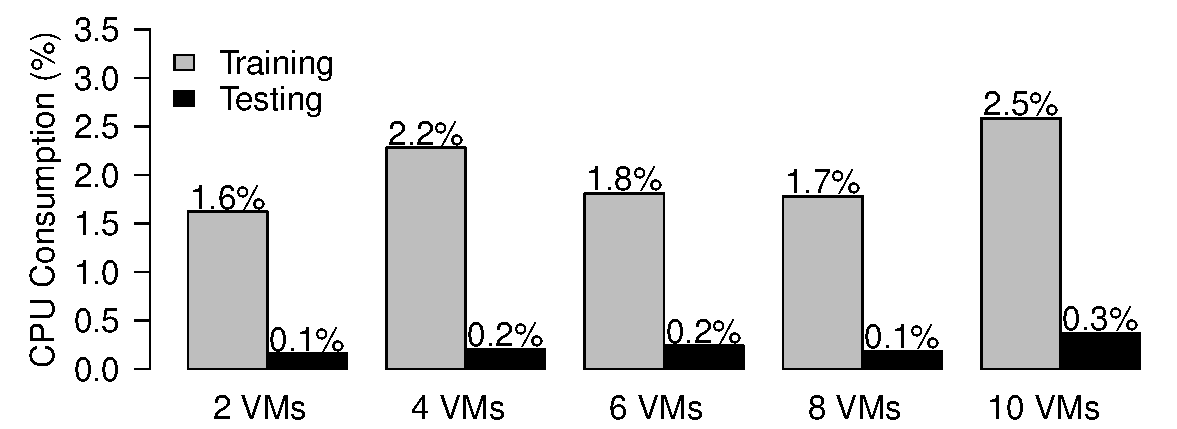
\epsfig{file = figures/overhead_cpu, width = 0.8\columnwidth}}
   \caption{Hosting node CPU consumption by RADS}
  \label{fig:overhead_cpu}
  \vspace{-0.1cm}
\end{figure}
%\vfill

% RAIDS TRAINING AND TESTING TIME
%\vfill
\begin{figure}[!h]
  \vspace{-0.2cm}
  \centering
   {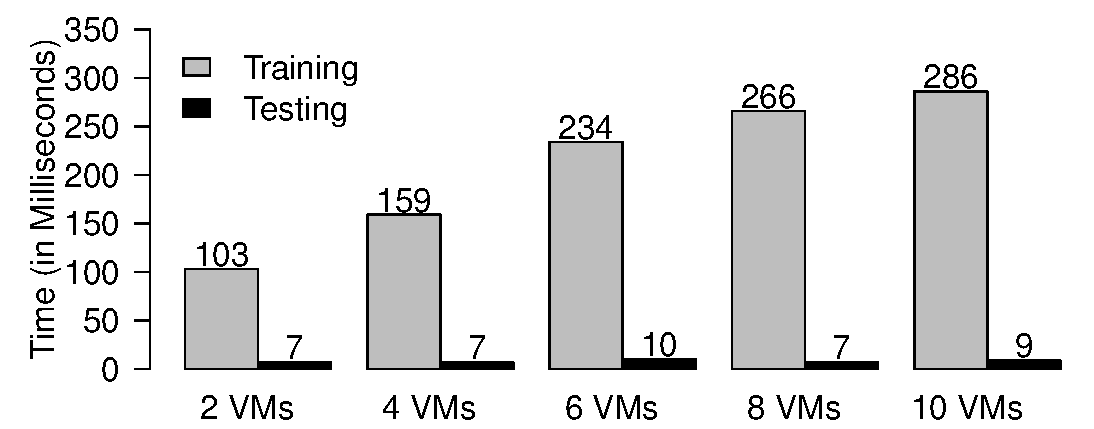
\epsfig{file = figures/overhead_time, width = 0.8\columnwidth}}
   \caption{Training and testing time required by RADS}
  \label{fig:overhead_time}
  \vspace{-0.1cm}
\end{figure}
%\vfill

\textit{Computation cost of RADS:} We measured the computation cost of RADS in terms of its CPU consumption on the hosting node. 
The bar plots in Figure~\ref{fig:overhead_cpu} show the CPU consumed by RADS while performing the training and the testing (anomaly detection).
From the plots we find that for training, the CPU consumption remains very low (in the range 1.6\% to 2.5\%) and it does not increase much with the scaling up of the number of VMs, whereas for testing, the CPU consumption remains consistently negligible. 
%We further found that for data collection, RAIDS consumed a very negligible amount of CPU (around 0.02\%).

\textit{Processing time of RADS}: The bar plots in Figure~\ref{fig:overhead_time} show the processing time that RADS took while performing the training and the testing. From the plots we observe that RADS took milliseconds in finishing the training and the testing tasks. The testing time is much lower than the training time. 
The training time increases with the scaling up of the number of VMs, but the testing time remains almost constant. 

In answering the research question 3, we can summarise that RADS can be used as a lightweight tool in terms of consuming minimal hosting node CPU and processing time in a Cloud data centre. However, the processing time required for training increases with the scaling up of the number of hosted VMs. This may lead to a RADS efficiency issue in the case where there are hundreds or thousands of hosted VMs and when the duration of the training increases to few hours or days. In future, we will attempt to explore this issue and address it with shared-memory or multithreaded programming solutions such as OpenMP, MPI, Phoenix++, etc.
%
%In answering the research question 3, we summarise the above observations as follows:
%\begin{enumerate}[{(a)}]
%\item RADS consumes minimal hosting node CPU during both training and testing. RADS can maintain its efficiency in terms of its CPU consumption even when there is scaling up of the number of hosted VMs.
%\item RADS processing time is minimal, however, the time required for training increases with the scaling up of the number of hosted VMs. This may lead to RADS efficiency issue in case when there are hundreds and thousands of hosted VMs and when the number of training data samples increase to few hours or days. 
%%However, the impact of such an issue should not persist long due to the fact that the training for a particular cloud application behaviour runs every 5 minutes and it stops when the RAIDS training optimiser algorithm (discussed in Section~\ref{sec:algorithm}) decides that the OCC model for that application is correctly built. Nevertheless, 
%In future, we will attempt to explore this issue and address it with shared-memory or multithreaded programming solutions such as OpenMP, MPI, Phoenix++ etc.
%\end{enumerate}

%\subsection{Evaluation of RAIDS Using Real-world Cloud Workload Trace}
\subsection{Real-world Experiments}
\label{sec:offline_analysis}
%In this section we evaluate the performance of RADS in terms of dealing with the genuine workload spikes observed in the real-world Cloud data centre workload trace. 
\noindent In this section we evaluate the performance of RADS in terms of false positive rate by analysing real-world Cloud workload traces. Specifically, in this section we attempt to answer research question 4.

%\subsubsection{Real-world Cloud Workload Trace Description}
%There are studies of Cloud workload traces such as~\cite{azure:2017}, \cite{Google:2012}, \cite{IBM:2014}, \cite{yahoo:2011}, \cite{FB:2012} which analysed the online traces collected from giant datacenter operators such as Microsoft, Google, IBM, Yahoo, Facebook etc. These traces do not represent Cloud data centre workloads in general; rather they represent workloads which may be typical for operations specific to these companies. Moreover, these studies do not include information regarding network traffic of the VMs, which is one of the metrics that we consider in RAIDS. 
%Therefore, as the real-world Cloud workload trace we used the traces from~\cite{workloadCCGRID:2015}. These traces are collected from a Cloud data centre named Bitbrains\footnote{https://www.solvinity.com}, which specialises in managed hosting and business computation for enterprises such as banks, credit card operators, insurers etc. Thus, the traces represent business critical workloads which generally use the same VM for long period of time. This is an important aspect for evaluating RAIDS performance as RAIDS assumes that for each VM, the application running during the testing period is the same application that was running during the training period. 
%The traces contain seven performance metrics including CPU utilisation and network throughput of 1,750 VMs from Bitbrains. The metrics are sampled every 5 minute. The traces were collected between July and September 2013 in two trace directories: (i) \textit{fastStorage} which consists of 1,250 VMs that are connected to fast storage area network (SAN) storage devices and (ii) \textit{Rnd} which consists of 500 VMs that are either connected to the fast SAN devices or to much slower Network Attached Storage (NAS) devices. \textit{fastStorage} contains one months of trace (August, 2013), whereas \textit{Rnd} contains three months of trace (July-September, 2013).
%\subsubsection{Real-world Cloud Workload Trace Description}
%\subsubsection{Trace Description}
\textbf{Trace Description:}
%RADS uses application-specific behavioural models to detect behavioural anomalies inside the VMs occurring due to security attacks. 
%Therefore, RAIDS can achieve maximum accuracy only when the VMs run the same Cloud application or workload throughout the training and the testing/detection phase. In order to obtain traces collected from VMs running the same Cloud application throughout the trace collection period, we carried out an investigation on available real-world Cloud workload traces. 
%In order to obtain the real-world Cloud workload traces, we carried out an investigation on available real-world Cloud workload traces. 
We selected the traces collected from a Cloud data centre named Bitbrains\footnote{https://www.solvinity.com} as analysed in~\cite{workloadCCGRID:2015}. % to use them as the real-world Cloud workload trace. 
Bitbrains specialises in managed hosting and business computation for enterprises such as banks, credit card operators, insurers, etc. 
%Researchers in~\cite{azure:2017, Google:2012, IBM:2014, yahoo:2011, FB:2012} analysed the real-world Cloud workload traces collected from giant datacenter operators such as Microsoft, Google, IBM, Yahoo, Facebook etc. These traces do not represent Cloud data centre workloads in general; rather they represent workloads which may be typical for operations specific to these companies. Moreover, these studies do not include information regarding network traffic of the VMs, which is one of the metrics that we consider in RADS. 
%The work in~\cite{workloadCCGRID:2015} analysed the traces collected from a Cloud data centre named Bitbrains\footnote{https://www.solvinity.com}, which specialises in managed hosting and business computation for enterprises such as banks, credit card operators, insurers etc. 
%Thus, these traces represent business critical workloads which generally use the same VM for long periods of time. 
%Based on our investigation, we selected the traces collected from Bitbrains as analysed in~\cite{workloadCCGRID:2015} to use them as the real-world Cloud workload trace. 
%These traces were collected from a Cloud data centre named Bitbrains\footnote{https://www.solvinity.com}, which specialises in managed hosting and business computation for enterprises such as banks, credit card operators, insurers etc. Thus, the traces represent business critical workloads which generally use the same VM for long period of time. 
%This is an important aspect for evaluating RAIDS performance as RAIDS assumes that for each VM, the application running during the testing period is the same application that was running during the training period. 
The traces contain seven performance metrics including CPU utilisation and network throughput of 1,750 VMs. The metrics are sampled every 5 minutes. The traces were collected between July and September 2013 in two trace directories: (i) \textit{fastStorage} which consists of 1,250 VMs that are connected to fast storage area network (SAN) storage devices and (ii) \textit{Rnd} which consists of 500 VMs that are either connected to the fast SAN devices or to much slower Network Attached Storage (NAS) devices. \textit{fastStorage} contains one month of trace (August, 2013), whereas \textit{Rnd} contains three months of trace (July-September, 2013).
%As we had limited knowledge of these traces, we could not choose the VMs which run the same application consistently throughout the data collection period. However, 
%We selected three consecutive days of traces to make an assumption that the Cloud applications or workloads running inside the VMs are consistent throughout the experimental period. 
%Therefore, RAIDS is designed for detecting security attacks on VMs which run the same Cloud application continuously throughout the training and the testing phase of RAIDS. 
 %that for each VM, the application running during the testing period is the same application that was running during the training period. 
%There are studies of Cloud workload traces such as~\cite{azure:2017}, \cite{Google:2012}, \cite{IBM:2014}, \cite{yahoo:2011}, \cite{FB:2012} which analysed the online traces collected from giant datacenter operators such as Microsoft, Google, IBM, Yahoo, Facebook etc. These traces do not represent Cloud data centre workloads in general; rather they represent workloads which may be typical for operations specific to these companies. Moreover, these studies do not include information regarding network traffic of the VMs, which is one of the metrics that we consider in RAIDS. 
%Therefore, as the real-world Cloud workload trace we collected the traces from~\cite{workloadCCGRID:2015}. These traces are collected from a Cloud data centre named Bitbrains\footnote{https://www.solvinity.com}, which specialises in managed hosting and business computation for enterprises such as banks, credit card operators, insurers etc. Thus, the traces represent business critical workloads which generally use the same VM for long period of time. 
%%This is an important aspect for evaluating RAIDS performance as RAIDS assumes that for each VM, the application running during the testing period is the same application that was running during the training period. 
%The traces contain seven performance metrics including CPU utilisation and network throughput of 1,750 VMs from Bitbrains. The metrics are sampled every 5 minute. The traces were collected between July and September 2013 in two trace directories: (i) \textit{fastStorage} which consists of 1,250 VMs that are connected to fast storage area network (SAN) storage devices and (ii) \textit{Rnd} which consists of 500 VMs that are either connected to the fast SAN devices or to much slower Network Attached Storage (NAS) devices. \textit{fastStorage} contains one months of trace (August, 2013), whereas \textit{Rnd} contains three months of trace (July-September, 2013).

%\subsubsection{Preparation of Traces}
\textbf{Preparation of Traces:}
\label{sec:preparaiton_of_traces}
In order to use the traces from~\cite{workloadCCGRID:2015} for evaluating the performance of RADS, we made the following selection process:
\begin{enumerate}[{(1)}]
\item We selected only the traces from the month August, 2013 for which both the traces (\textit{fastStorage} and \textit{Rnd}) were available. 
\item We further selected the first three days of traces, making the assumption that the Cloud applications or workloads running inside the VMs are consistent throughout the experimental period. 
%\item We further selected only the first three days of traces for ease of experiment. 
%\item We further selected only the first three days of traces so that we can make the following assumption: \textit{throughput the lifetime of the trace collection each monitored VM executed only a single application and that application continued to run in the same VM.}
\item Out of the three days of traces, we selected the first two days (14:40, 12 August to 14:40, 14 August 2013) of traces for training and and the third day (14:40, 14 August to 14:40, 15 August 2013) of traces for testing. 
\item We performed spike detection analysis on the traces using the Interquartile Range (IQR\footnote{https://en.wikipedia.org/wiki/Interquartile\_range}) algorithm and selected traces only from VMs which flagged spikes. This is because we intend to evaluate the performance of RADS in terms of dealing with the genuine workload spikes observed in the traces. 
\item Finally, for CPU utilisation analysis, we selected traces from VMs which have CPU utilisation greater than 10\%, and for network throughput analysis we selected the traces from VMs with network throughput greater than 100KB/s. This is done in order to select traces from active VMs which are running a decent amount of workload. 
%Thus, we selected the traces from 82 VMs for CPU utilisation analysis and 212 VMs for network throughput analysis. 
\end{enumerate}

Following the above selection process, we chose the traces from 82 VMs for CPU utilisation analysis and traces from 212 VMs for network throughput analysis.

% OFFLINE  TIMESERIES GRAPHS
%\vfill
\begin{figure}[!h]
  %\vspace{-0.2cm}
  \centering
   {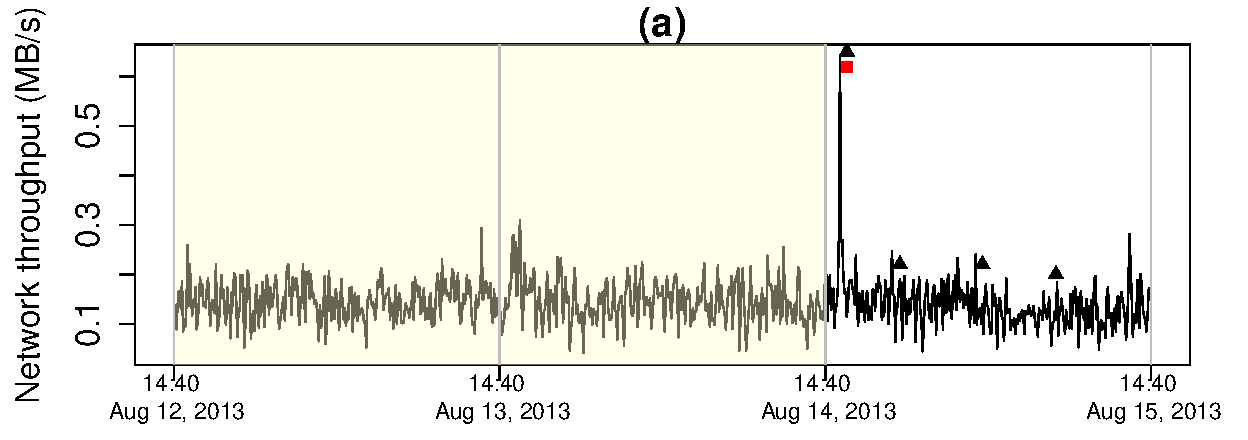
\epsfig{file = figures/realworld_network_941, width = 0.8\columnwidth}}
    {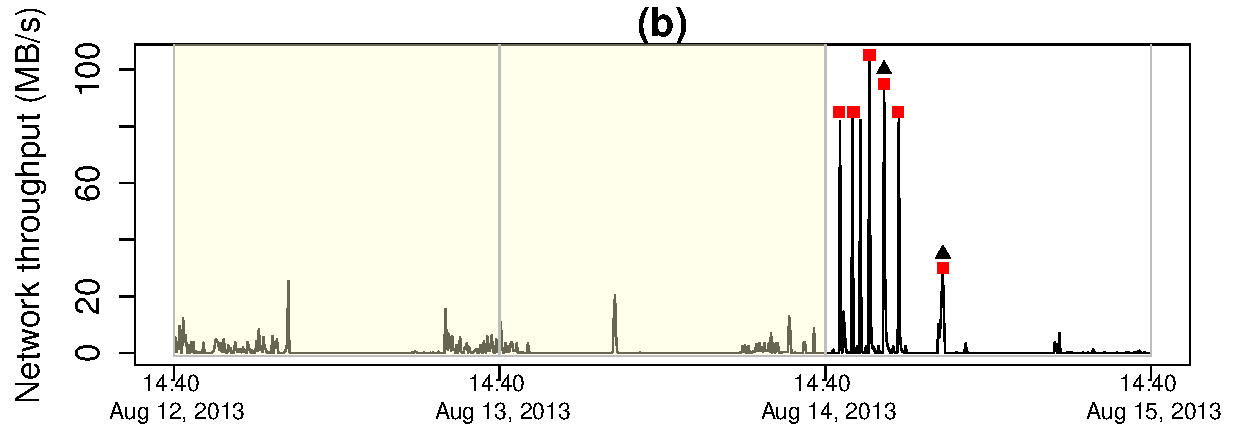
\epsfig{file = figures/realworld_network_357, width = 0.8\columnwidth}}
      {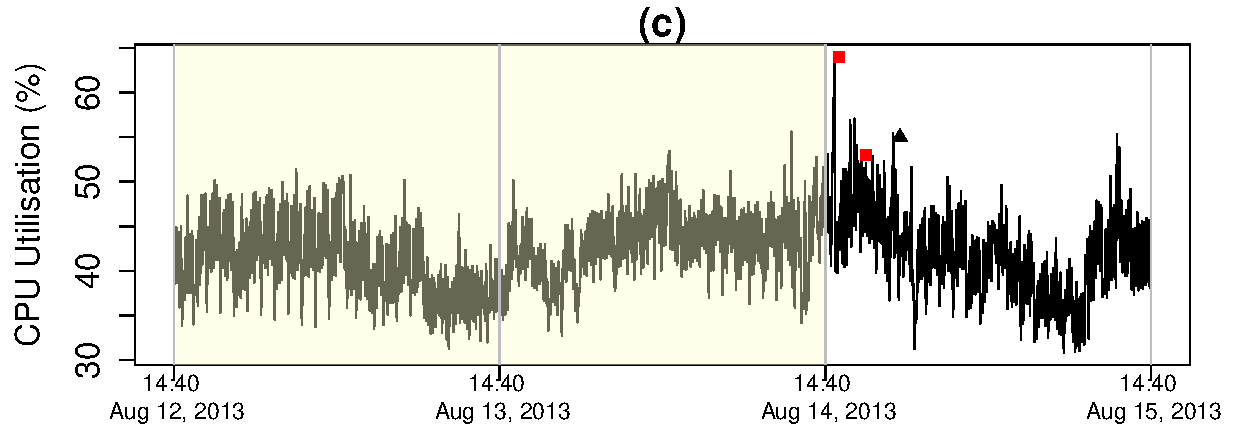
\epsfig{file = figures/realworld_cpu_980, width = 0.8\columnwidth}}
         {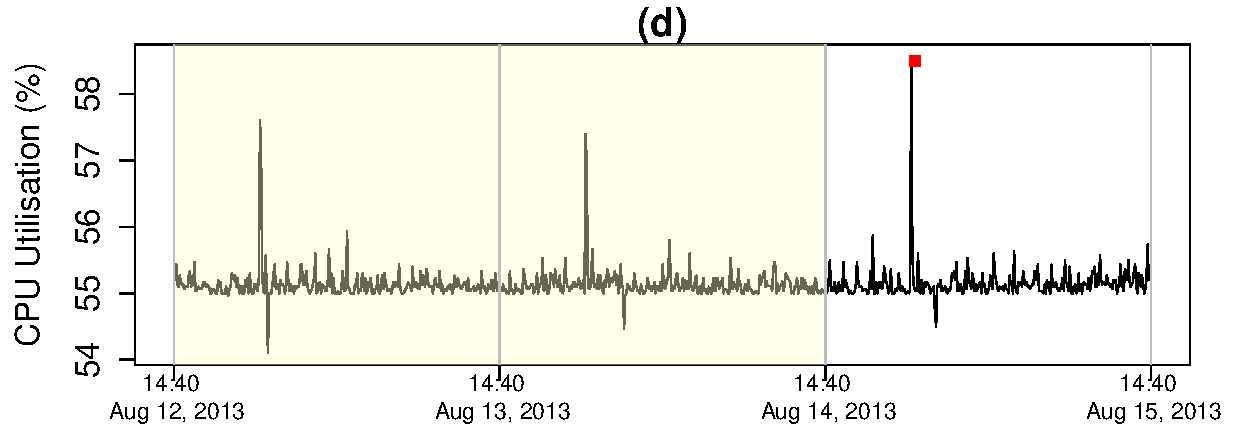
\epsfig{file = figures/realworld_cpu_1556, width = 0.8\columnwidth}}
           % {\epsfig{file = figures/realworld_network_1025, width = \columnwidth}}
  % \caption{Performance of RAIDS on different VM traces collected from the Grid Workload Archives [ref]: (a) VM-941 from fastStorage trace, (b) VM-357 from fastStorage trace, (c) VM-980 from fastStorage trace, (d) VM-306 from Rnd trace, (e) VM-1025 from fastStorage trace. The yellow coloured section represent the training period and the section without colour represents the testing period. The coloured shapes represent false alarms while using different data pre-processing approaches by RAIDS: blue round, red square, and black triangle are for average and standard deviation based approach, average based approach, and entropy based approach respectively. }
%      \caption{Responses from RAIDS on different Cloud workload behaviour observed in the traces collected from~\cite{workloadCCGRID:2015}: (a) VM-941 from fastStorage trace, (b) VM-357 from fastStorage trace, (c) VM-980 from fastStorage trace, (d) VM-306 from Rnd trace, (e) VM-1025 from fastStorage trace. The yellow coloured sections represent the training period and the section without colour represents the testing period. The coloured shapes represent ``anomaly" alarms raised by RAIDS while using different data pre-processing approaches: blue round, red square, and black triangle are for proposed approach (average and standard deviation based approach), average based approach, and entropy based approach, respectively. }
      
          % \caption{Responses from RADS on different Cloud workload behaviour observed in the traces collected from~\cite{workloadCCGRID:2015}: (a) VM-941 from fastStorage trace, (b) VM-357 from fastStorage trace, (c) VM-980 from fastStorage trace, (d) VM-306 from Rnd trace. The yellow coloured sections represent the training period and the section without colour represents the testing period. The coloured shapes represent ``anomaly" alarms raised by RADS while using different data pre-processing approaches: red square and black triangle are for the average and the entropy based approaches, respectively. }
           
                      \caption{RADS analysis of different Cloud workload behaviour observed in the traces collected from~\cite{workloadCCGRID:2015}: (a) VM-941 from fastStorage trace, (b) VM-357 from fastStorage trace, (c) VM-980 from fastStorage trace, (d) VM-306 from Rnd trace. The yellow coloured section represents the training period and the section without colour represents the testing period. The coloured shapes represent ``anomaly" alarms raised by RADS while using different time series analyses: red square and black triangle are for the average and the entropy based analysis, respectively. }



  \label{fig:offline_timeseries}
  %\vspace{-0.1cm}
\end{figure}
%\vfill


%\subsubsection{Performance of RADS Under Different Cloud Workload}
\textbf{Performance of RADS Under Different Cloud Workloads:}
%Out of the selected traces, we chose the traces from certain VMs, which experience different workload behaviour as presented in Figure~\ref{fig:offline_timeseries} using the timeseries graphs.
%In the figure, the left two yellow coloured sections represent the training period trace with which we trained the RAIDS classifier, whereas the right section without any colour represent the testing period trace for which we observe the responses from RAIDS. 
%\begin{enumerate}[{(a)}]
%\item \textit{VM-941 from fastStorage trace}: Figure~\ref{fig:offline_timeseries}(a) shows the network throughput for VM-941 collected from \textit{fastStorage} trace. From the figure we observe that the network throughput for this VM is consistently fluctuating throughput the training and the testing period and there is one significant genuine workload spike occurring during the testing period. 
%\item \textit{VM-357 from fastStorage trace} (Figure~\ref{fig:offline_timeseries}(b)): Figure~\ref{fig:offline_timeseries}(b) shows the network throughput for VM-357 collected from \textit{fastStorage} trace. 
%From the figure we observe that the network throughput for this VM is irregularly fluctuating throughput the training and the testing period and there are multiple significant genuine workload spikes occurring during the testing period.
%\item \textit{VM-980 from fastStorage trace} (Figure~\ref{fig:offline_timeseries}(c)): consistently fluctuating CPU utilisation behaviour during both the training and the testing period. Multiple insignificant genuine workload spike occurring during the testing period. 
%\item \textit{VM-306 from Rnd trace} (Figure~\ref{fig:offline_timeseries}(d)): consistently fluctuating CPU utilisation behaviour during both the training and the testing period. Insignificant genuine workload spike occurring during the both the training and the testing period. 
%\item \textit{VM-1025 from fastStorage} (Figure~\ref{fig:offline_timeseries}(e)):  irregularly fluctuating network behaviour during the training period. Multiple genuine behavioural change during the testing period with occasional genuine workload spikes.  
%\end{enumerate}
Out of the selected traces, we chose the traces from a range of VMs exhibiting varying workload behaviour as presented in Figure~\ref{fig:offline_timeseries} using the time series graphs. 
%The timeseries graphs reveal how RAIDS responses towards these workload behaviour while using different data pre-processing approaches. We summarise the observations from these graphs as follows.}
The time series graphs reveal how RADS performs under different Cloud workload behaviour while using different time series analyses. We summarise the observations from these graphs as follows:

\begin{enumerate}[{(a)}]
\item In both cases where the workload experiences consistently fluctuating behaviour (Figure~\ref{fig:offline_timeseries}(a)) and irregular behaviour (Figure~\ref{fig:offline_timeseries}(c)), RADS successfully classifies the genuine workload spikes as ``normal" while using its window-based time series analysis. But, while using the average or the entropy based analysis, RADS fails to classify the genuine workload spikes as ``normal" and raises false ``anomaly" alarms. %In fact using the entropy based approach raises three more false alarms. 
\item In both the cases where the workload experiences significant genuine workload spikes (Figures~\ref{fig:offline_timeseries}(a) and (b)) and insignificant genuine workload spikes (Figure~\ref{fig:offline_timeseries}(c)), RADS successfully classifies them as ``normal" while using its window-based time series analysis.  But, while using the average or the entropy based analysis RADS fails to classify them as ``normal" and raises false ``anomaly" alarms.
\item While using its window-based time series analysis, RADS continues its successful classification of genuine workload spikes as ``normal" even when the workload experiences genuine workload spikes during the training period (Figure~\ref{fig:offline_timeseries}(d)). However, using the average based analysis RADS fails again to classify the genuine workload spikes as ``normal" and raises false ``anomaly" alarm. 
%\item During the testing period, when the workload experiences significant behavioural change, which persist for a relatively long period of time (Figure~\ref{fig:offline_timeseries}(e)), RADS can successfully classify that change and raise ``anomaly" alarms while using all the data pre-processing approaches that we consider. 
%This gives us the indication that using the proposed data pre-processing approach, RADS can not only deal with the genuine workload spikes (which persist only for a momentary period of time) but also it can successfully detect the ``anomalies" occurring due to the cybersecurity attacks (which persist for a relatively long period of time).
%\item When the workload experiences significant and consistent behavioural change during the testing period (Figure~\ref{fig:offline_timeseries}(e)), RAIDS can successfully classify that change and raise ``anomaly" alarms while using all the data pre-processing approaches that we consider. 
%\textcolor{blue}{This gives us the indication that using the proposed data pre-processing approach, RAIDS can not only deal with the genuine workload spikes but also it can successfully detect the ``anomalies" occurring due to the security attacks. This is because genuine workload spikes are differentiated from the security attacks by considering the fact that spikes persist only for a momentary period of time, whereas security attacks persist for a relatively long period of time.}
\end{enumerate}

% RAIDS VERSIONS  TABLE
%\newcolumntype{L}[1]{>{\raggedright\arraybackslash}p{#1}}
%\newcolumntype{C}[1]{>{\centering\arraybackslash}p{#1}}
%\newcolumntype{R}[1]{>{\raggedleft\arraybackslash}p{#1}}
%\begin{table}[t]
%%\caption{Different versions of RAIDS using different data pre-processing approaches and different number of artificial data points}
%\caption{Different experiments performed for RADS}\
%%\caption{Experiment details}
%\label{tab:raids_versions} 
%\centering
%%\begin{tabular}{|c|c|}
%\begin{tabular}{C{1cm}C{4cm}C{2.8cm}} %C{1.5cm}}
%  \toprule
%   Experiment & Data Pre-processing Approach & Artificial Data Points \\ %& Overall detection accuracy \\
%    \bottomrule
%        \begin{tabular}{C{0.7cm}} RADS1 \\ RADS2 \\ RADS3 \\ AVG \\ ENT \\  \end{tabular} 
%        & \begin{tabular}{C{3.7cm}} Average \& Standard Deviation \\ Average \& Standard Deviation \\ Average \& Standard Deviation \\ Average \\ Entropy \end{tabular} 
%        & \begin{tabular}{C{2.7cm}}  1x of raw data points \\  2x of raw data points \\  3x of raw data points \\ No artificial data points \\ No artificial data points \end{tabular} \\
%       
%    \hline
%      
%\end{tabular}
%\end{table}

% END OF RAIDS VERSIONS  TABLE

% OFFLINE CPU AND NETWORK ANALYSIS
%\vfill
\begin{figure}[!h]
%  \vspace{-0.2cm}
  \centering
   {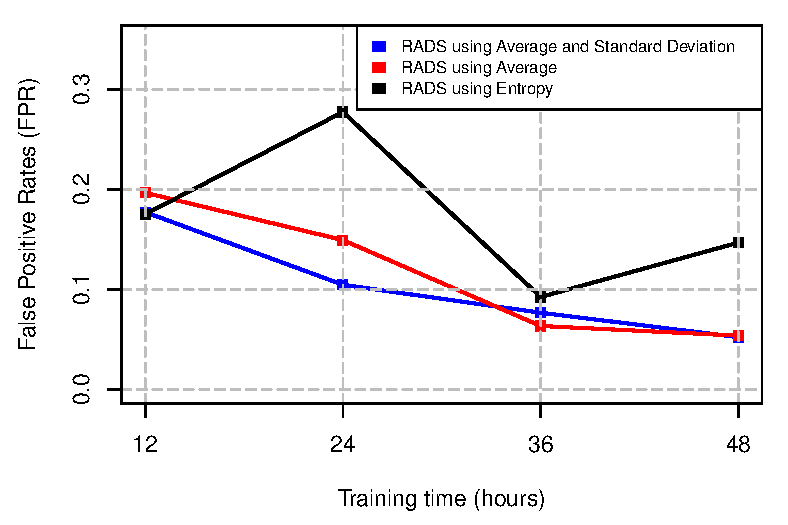
\epsfig{file = figures/offline_cpu_24, width = 0.7\columnwidth}}
      {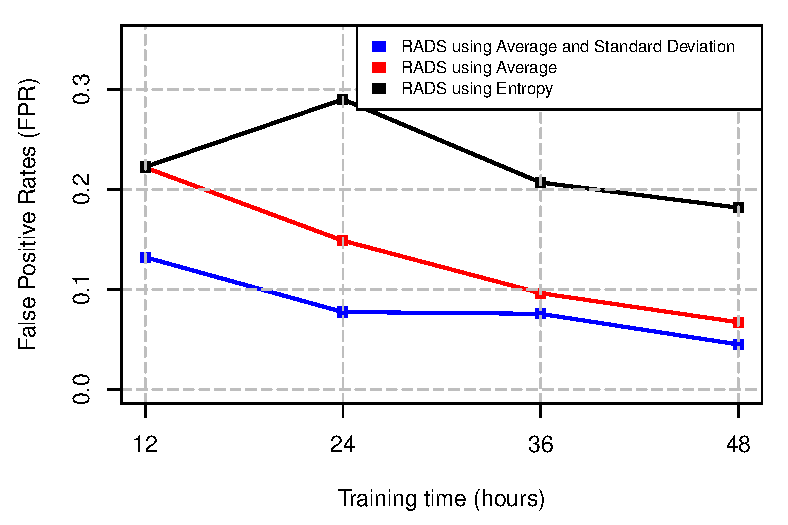
\epsfig{file = figures/offline_network_24, width = 0.7\columnwidth}}
     % {\epsfig{file = figures/offline_cpu_improvement, width = \columnwidth}}
   \caption{False Positive Rates (FPR) while running experiments on CPU utilisation (above) and network throughput (bottom)}
     % \caption{False positive rates of different versions of RAIDS while analysing CPU utilisation. (Below) Percentage of the performance improvement of RAIDS1/RAIDS2/RAIDS3 over average and entropy }
  \label{fig:offline_cpu_network}
 % \vspace{-0.1cm}
\end{figure}
%\vfill


%\subsubsection{Overall Performance of RADS}
\textbf{Overall Performance of RADS:}
%In the previous section we analysed the traces only from certain VMs in order to observe RAIDS responses towards varying Cloud workload behaviour. 
%We evaluate the overall performance of RAIDS in terms of dealing with the genuine workload spikes while analysing the traces chosen based on the selection process described in Section~\ref{sec:preparaiton_of_traces}. 
We evaluate the overall performance of RADS in terms of false positive rate. 
%by analysing the real-world Cloud workload traces. 
%chosen based on the selection process described in Section~\ref{sec:preparaiton_of_traces}. 
%This evaluation process considers different versions of RAIDS based on the number of artificial data points (required to deal with the genuine workload spikes as described in Section~\ref{sec:approach}) and the data pre-processing approach that it uses. The versions are defined in Table~\ref{tab:raids_versions}. Figure~\ref{fig:offline_cpu_network} presents the result of the False Positive Rates (FPR, calculated using the Equation~\ref{eq5}) of different versions of RAIDS while running tests on CPU utilisation trace of 82 VMs and network throughput trace of 212 VMs, which are collected from~\cite{workloadCCGRID:2015}. The tests are performed with 1 day (24 hours) of testing trace. Details of the training and the testing trace selection are presented in Section~\ref{sec:preparaiton_of_traces}.
%Specifically, in this evaluation process we performed different experiments for RADS based on the number of artificial data points and the data pre-processing approaches. The experiments are defined in Table~\ref{tab:raids_versions}. 
%As described in Section~\ref{sec:approach}, artificial data points are required to deal with the genuine workload spikes.  
%While describing the RADS framework in Section~\ref{sec:framework}, we consider the number of artificial data points to be equal to the total number of raw data points. To support this consideration, in this section we explore various numbers of artificial data points which are multiples of the total number of raw data points. 
% the optimal number of artificial data points for RAIDS. 
%The experiments with varying number of artificial data points are performed in order to decide the optimal number of artificial data points for RAIDS. 
Figure~\ref{fig:offline_cpu_network} presents the results of the False Positive Rates (FPR, calculated using Equation~\ref{eq5}) of RADS while running the experiments on a CPU utilisation trace of 82 VMs and a network throughput trace of 212 VMs.
%, 
%which are collected from~\cite{workloadCCGRID:2015}. 
%which were chosen based on the selection process described in Section~\ref{sec:preparaiton_of_traces}.
The experiments were performed with 24 hours of testing trace. 
%Details of the training and the testing trace selection process are presented in Section~\ref{sec:preparaiton_of_traces}.
%It is important to note that the traces from~\cite{workloadCCGRID:2015} does not include the information regarding the arrival processes, which can indicate the lifetime of user applications or VMs. Therefore, although the traces from~\cite{workloadCCGRID:2015} represent business critical workloads which generally use the same VM for a long period of time, we cannot verify whether the VMs under examination validate the assumption that we made in Section~\ref{sec:preparaiton_of_traces}: \textit{throughput the lifetime of the trace collection each monitored VM executed only a single application and that application continued to run in the same VM}. 
%Thus, the result that is presented in Figure~\ref{fig:offline_cpu_network} may not evaluate the performance of RAIDS correctly for the VMs which run variable or inconsistent user applications.
%we are not sure about which of the VMs under our examination run the same user application throughput the experimental period of 3 days. Thus, the result that is presented in Figure~\ref{fig:offline_cpu_network} may not evaluate the performance of RAIDS correctly for the VMs which run variable or inconsistent user applications. }
%the information regarding the Cloud applications running inside the selected VMs are not known and therefore its not 
% Similarly, Figure~\ref{fig:offline_network} presents the result of the FPR of different versions of RAIDS while analysing network throughput trace of 212 VMs collected from~\cite{workloadCCGRID:2015}. 
%The figures also present the percentage of the performance improvement (in terms of dealing with false positives) of RAIDS1/RAIDS2/RAIDS3 (we chose the best one amongst these in each occasion) over average and entropy.
We summarise the observations from the results as follows:
\begin{enumerate}[{(a)}]
%\item In case of both the experiments running on CPU utilisation and network throughput trace, all the versions of RAIDS achieve better performance (lower value of FPR means better performance) with the increase in the training time. This emphasises further the requirement of the proposed Training Optimiser Algorithm (Algorithm~\ref{raids_algorithm_training_optimiser}), which can decide the optimal training time.
%\item Results obtained from running experiments on both CPU utilisation and network throughput trace show that in most occasions RAIDS achieves better performance (lower value of FPR means better performance) with increase in training time and at one stage (training time - from $36$ to $48$ hours) the performance starts becoming stable. These results emphasise further the requirement of the proposed Training Optimiser Algorithm (Algorithm~\ref{raids_algorithm_training_optimiser}), which can decide the optimal training time.
\item On most occasions, when RADS uses its window-based time series analysis (combination of average and standard deviation), it achieves better performance (lower value of FPR means better performance) with increase in training time and at one stage (training time - from $36$ to $48$ hours) the performance starts becoming stable. These results emphasise further the requirement of the proposed training optimisation algorithm (Algorithm~\ref{raids_algorithm_training_optimiser}), which can decide the optimal training time.
\item The performance of RADS while using its window-based time series analysis is better than the performance of RADS while using average and entropy based analysis on most occasions.
% except for training time $36$ hours in case of CPU utilisation analysis where average based analysis performs slightly better than the window-based time series analysis of RADS. }
%\item The performance of RADS in case of RADS1, RADS2, and RADS3 (all using the proposed data pre-processing approach based on average and standard deviation) is better than the performance of RADS in case of AVG (using the average based data pre-processing approach) and ENT (using the entropy based data pre-processing approach) on most occasions (training time - $24, 36, 48$ hours). The performance of RADS is always better in case of RADS1 (using 1x of raw data points as artificial data points) in comparison to the performance of RADS in case of AVG and ENT except for one occasion (training time - 36 hours in case of CPU utilisation) when the performance slightly degrades. 
%This observation along with the fact that the more the artificial data points RADS uses the more computation resource and time it will require for the training supports the use of 1x of raw data points as artificial data points, 
%\item The performance of RADS in case of RADS1, RADS2, and RADS3 (all using the proposed data pre-processing approach based on average and standard deviation) is better than the performance of RADS in case of AVG (using the average based data pre-processing approach) and ENT (using the entropy based data pre-processing approach) on most occasions (training time - $24, 36, 48$ hours). The performance of RADS is always better in case of RADS1 (using 1x of raw data points as artificial data points) in comparison to the performance of RADS in case of AVG and ENT except for one occasion (training time - 36 hours in case of CPU utilisation) when the performance slightly degrades. This observation along with the fact that the more the artificial data points RADS uses the more computation resource and time it will require for the training supports the use of 1x of raw data points as artificial data points, 
%i.e. the number of artificial data points is equal to the total number of raw data points.
%i.e. there is no merit in using a number of artificial data points which is greater than the number of raw data points.
%Moreover, this investigation is important because using artificial data points which are manyfold of the total number of raw data points may improve the performance of RAIDS, but this may bring efficiency issues in terms of resource consumption and processing time. }
%However, none of the RAIDS version amongst RAIDS1, RAIDS2, and RAIDS3 is performing the best in all occasions and therefore, we had to choose the best amongst these in each occasion while comparing against AVG and ENT in the bar plots depicting the percentage of performance improvement. Due to the same reason we do not conclude which RAIDS version amongst RAIDS1, RAIDS2, and RAIDS3 is the best, instead we use RAIDS1 and allow the proposed Training Optimiser Algorithm (Algorithm~\ref{raids_algorithm_training_optimiser}) to decide the training data points with which it can be trained to perform successfully. Selecting only RAIDS1 
%\item In case of CPU utilisation analysis, RAIDS2 and RAIDS3 achieves better than AVG and ENT when the training time is between 24-48 hours, whereas RAIDS1 achieves  better than AVG and ENT in all occasions except for training time 36 hours. In case of network throughput analysis, RAIDS1 
%\item The performance improvement of RAIDS (RAIDS1/RAIDS2/RAIDS3) is much higher in case of network throughput analysis (31-49\% over average and 40-75\% over entropy) in comparison to the performance improvement of RAIDS in case of CPU utilisation analysis. 
\end {enumerate}

%As mentioned earlier, due to the limited knowledge of the traces, we could not choose the VMs which run the same application consistently throughout the data collection period. As a result, the traces analysed above may include VMs which run inconsistent Cloud applications.
%and may result in poor performance for RAIDS. 
%If RADS is applied only to VMs which run the same Cloud application consistently, RADS may achieve better performance than what is observed above. 

%% OFFLINE NEWORK ANALYSIS
%%\vfill
%\begin{figure}[!h]
%  %\vspace{-0.2cm}
%  \centering
%   {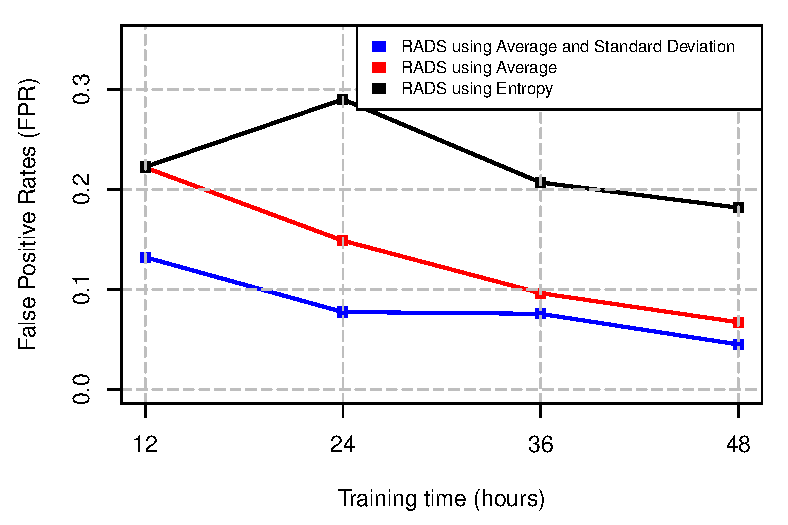
\epsfig{file = figures/offline_network_24, width = \columnwidth}}
%     % {\epsfig{file = figures/offline_network_improvement, width = \columnwidth}}
% %  \caption{(Above) False positive rates of different versions of RAIDS while analysing network throughput. (Below) Percentage of the performance improvement of RAIDS1/RAIDS2/RAIDS3 over average and entropy }
%    \caption{False positive rates of different versions of RAIDS while analysing network throughput}
%
%  \label{fig:offline_network}
% % \vspace{-0.1cm}
%\end{figure}
%%\vfill




\section{Related Work}
\label{sec:related_work}
%\noindent In recent years, researchers have proposed various anomaly-based IDSs for Cloud data centres, which implement machine learning algorithms. We discuss different types of machine learning algorithms used for Cloud anomaly detection as follows. 
\noindent In recent years, researchers have proposed various anomaly detection systems for Cloud data centres. We classify them based on the machine learning algorithms which they implement.

%\subsection {Cloud Intrusion Detection Systems (IDSs)}
\textit{(i) Supervised learning algorithms.}
Supervised learning algorithms rely on labelled training data to detect previously known anomalies. 
%Gupta and Kumar~\cite{Gupta:%2015:ISC:2738886.2738910} suggest an Immediate System Call pattern detection in order to track patterns in the system call logs which can identify a malicious program execution inside VMs. 
%In this case, the detection is not in real-time and the detection is only effective when there is a previously generated pattern of the immediate system calls of the monitored programs.
Li et al.~\cite{ml_based:2012} propose an Artificial Neural Network (ANN) based intrusion detection system for Cloud. The ANN algorithm learns the ``normal" and the ``anomalous" behaviour from a large dataset of VM network traffic. The learned ANN is capable of detecting Cloud security attacks with accurate results.
An anomaly detection system suitable for the hypervisor layer is proposed in~\cite{Pandeeswari2016}. The anomaly detection in this case is based on a mixture of Fuzzy C-Means clustering algorithm and Artificial Neural Network (FCM-ANN) which results in better accuracy and lower false positive rate than the classic ANN and Naive Bayes classifier for detecting various Cloud security attacks. 
The authors in~\cite{supervised_ml:2017} use Linear Regression (LR) and Random Forest (RF) algorithms to detect and categorise anomalies in a Cloud data centre. 
%Before using these machine learning algorithms they use a feature selection scheme to reduce the number of features required to build the machine learning model. This has improved the performance of the algorithms in terms of anomaly detection accuracy. 
%this paper, we investigate both detecting and categorizing anomalies rather than just detecting, which is a common trend in the contemporary research works. We have used a popular publicly available dataset to build and test learning models for both detection and categorization of different attacks. To be precise, we have used two supervised machine learning techniques, namely linear regression (LR) and random forest (RF). 
%However, this system requires a lot of training data due to the nature of the algorithms.
%An Intelligent IDS for Private Cloud Environment has been proposed in~\cite{B.2015}). This approach which utilises a hardware module and a software application is based on previous history of intrusion traces which are given to the system during a training phase.
%In \cite{al2015applying} an anomaly intrusion detection model has been proposed to deal with attacks and security violations in Cloud environments. The detection model is utilising Hopefield Artificial Network and Simulating Annealing as aggregator which results in a detection rate of 93\% or less.
Gulenko et al.~\cite{ML_based_ids:2016} exploit various machine learning algorithms to detect anomalies in Cloud host machines. They use a combination of two types of data sets for evaluating the algorithms: ``normal" operation data and ``anomalous" data obtained via anomaly injection. They train the machine learning models offline and use them to detect the anomalies at runtime. 
%The results from~\cite{ML_based_ids:2016} indicate that machine learning algorithms are able to predict cloud anomalies with high accuracy. However, authors observed that the models trained for the host machines are affected due to ageing effects. Accuracy of the algorithms was degraded while evaluating them by separating the training and the testing data by time. 
The supervised learning algorithms used in Cloud anomaly detection as discussed above require training of the machine learning models with both ``normal" and ``anomalous" traces. 
%They usually collect the ``anomalous" traces from online repositories or generate them artificially.  
%These algorithms may fail to detect novel attacks, which are not recorded by the learning models or which have very different patterns than the learned attack patterns. 
These algorithms may fail to detect anomalies due to unknown attacks, traces of which are not recorded by the learning models or which have very different patterns than the learned ``anomalous" patterns.
To solve this problem researchers have proposed unsupervised learning algorithms which we discuss next. The unsupervised learning algorithms do not require labelled training data, i.e. they can build the learning models without the ``anomalous" traces.  
%whose attack pattern are very much different than learned attack patterns. We now discuss below how anomaly detection techniques can be used to overcome this limitation:
%Anomaly-based IDSs are more acceptable than the signature-based IDSs due to their strength in detecting unknown security attacks, which do not have any samples available for producing rules or finding signatures for signature-based IDSs. Moreover,  the most common cloud intrusions such as DDoS attacks, attacks on the hypervisor or on the virtual machine typically cause disruption on the cloud system's normal utilisation of either network, a computational resource, storage or a virtual machine's functionality. Such disruptions can be successfully captured by an anomaly-based IDS to identify them as a cause of cloud intrusion. 

\textit{(ii) Unsupervised learning algorithms.}
The authors in~\cite{automated-detection:2016} propose a mechanism for automatic anomaly detection and root cause analysis for Cloud data centres. They use an unsupervised K-Means clustering algorithm to identify the ``abnormal" system behaviour. 
%They use CPU utilisation and network traffic data for the analysis. 
%By performing an emulated DDoS attack on a cloud tested, they showed that their mechanism accurately identifies cloud anomalies and their causes.
UBL proposed in~\cite{UBL:2012} uses an unsupervised Self Organising Map (SOM) algorithm to predict unknown anomalies. SOM is computationally less expensive than K-Nearest Neighbour~\cite{knearest:2005}. 
%UBL requires only system-level metrics (CPU, memory, network, IOPS) to achieve black-box anomaly prediction. 
UBL predicts anomalies by identifying early deviations from ``normal" system behaviour. 
%Experimental results in~\cite{UBL:2012} show that UBL can accurately predict performance anomalies with sufficient lead time to prevent the anomalies.
\cite{density-based:2016} proposes a Cloud anomaly detection technique based on the concept of data density introduced by~\cite{density-based_ref1:2011}, which implements non-parametric Cauchy function~\cite{density-based_ref2:2010}. 
This technique computes the density recursively and therefore, it is memory-less and unsupervised.  
%The authors in~\cite{density-based:2016} evaluated the performance of the proposed technique based on the emulated dataset from a testbed, under different types and intensities of attacks. with high accuracy. 
%The evaluation results show that the proposed technique can achieve high accuracy of detection.
The authors in~\cite{EbAT:2010}, \cite{entorpy_based_detection_2:2014} measure the entropy of the system metrics such as CPU, memory, network, IOPS, etc., in order to identify Cloud anomalies. The entropy values indicate the dispersal or concentration of the metric distributions and they form the time series data for anomaly analysis.
%In~\cite{EbAT:2010}, the metrics are aggregated by entropy distributions across the cloud stack in order to form entropy time series. 
%EbAT, proposed in~\cite{EbAT:2010}, uses online tools like spike detection, signal processing and subspace methods to detect anomalies in the entropy time series. 
The approach proposed in~\cite{entorpy_based_detection_2:2014} identifies a Cloud security attack by observing whether the entropy variables obey normal distribution or not. They use Kolmogorov-Smirnov test (K-S test) to identify whether the entropy variables obey normal distribution. 
%When the Cloud data centre encounters an intrusion, the entropy variables do not obey normal distribution, which indicates an ``anomaly" due to attack. 
%Both ~\cite{EbAT:2010} and \cite{entorpy_based_detection_2:2014} can detect the cloud anomalies with high accuracy.
Recently, entropy has been used in various network anomaly detection tools~\cite{entorpy_based_detection_1:2005}, \cite{entorpy_based_detection_5:2014}, \cite{entorpy_based_detection_3:2017}, \cite{entorpy_based_detection_4:2017}. These tools firstly measure the entropy associated with the network traffic or network packet features (IP addresses and ports) and secondly they detect network attacks by observing the variation in the entropy values.
In our previous works~\cite{ladt:2015, ls-ladt:2016} we proposed a Lightweight Anomaly Detection Tool (LADT) which can detect anomalies on the hosting node level by using a correlation based algorithm. The algorithm utilises performance metrics on the hosting node level and the VM level to track disparities on the resource usage and detect host level attacks such as a Blue Pill attack~\cite{bluepill:2006}. However, this approach is not able to detect anomalies in the VM level which is the case for the current paper.

Although the unsupervised learning algorithms discussed above can detect Cloud anomalies due to unknown security attacks with high accuracy, they may generate false positives which arise mainly due to the workload spikes in a Cloud data centre.
%suffer from false alarm issues generated due to the wrong identification of the genuine Cloud workload spikes as ``anomalies". 
%Some algorithms~\cite{cloud-malware:2016}, \cite{automated-detection:2016}, \cite{UBL:2012} consider pre-processing the raw data using averaging in order to reduce false positives, but that is not sufficient. 
%The proposed anomaly detection system in this paper (RADS) uses One Class Classification (OCC) algorithm that is proposed by Hempstalk et al. in~\cite{OCC:2008}.
%and implements a window based data pre-processing approach which considers both the average and standard deviation of the raw data. RAIDS data pre-processing approach provides better accuracy and false alarm rate than the state-of- the-art average or entropy based data pre-processing approaches.
%RAIDS provides better accuracy and false alarm rate while using its data pre-processing approach, instead of using the state-of- the-art average or entropy based data pre-processing approaches.
%RAIDS uses the One Class Classification (OCC) algorithm that is proposed by Hempstalk et al. in~\cite{OCC:2008} to detect Cloud anomalies arising due to unknown security attacks. 
%In the literature, we find only the work in~\cite{cloud-malware:2016} that uses OCC algorithm for Cloud intrusion detection; specifically 
The authors in~\cite{cloud-malware:2016} propose a novel approach for Cloud malware detection using one class Support Vector Machine (SVM) algorithm. One class SVM is an extension of the traditional two-class SVM, which was proposed by Sch\"{o}lkopf et al. in~\cite{one_class_svm:1999}. 
Similar to the OCC algorithm~\cite{OCC:2008} that is used in this paper, one class SVM takes the unlabelled training data and produces a binary class based on the distribution of the training data. The binary class is composed of a known class, which is the ``normal" VM behaviour and a novel class, which is the unknown class representing the ``anomalous" instances. 
The work in this paper is different from that in~\cite{cloud-malware:2016} as this work focuses more on increasing the accuracy while reducing the false positives arising due to genuine Cloud workload spikes; whereas, \cite{cloud-malware:2016} focuses on reducing false positives arising due to VM live-migration.
%Some algorithms~\cite{cloud-malware:2016}, \cite{automated-detection:2016}, \cite{UBL:2012} consider pre-processing the raw data using averaging in order to reduce false positives, but that is not sufficient. 
%The proposed anomaly detection system in this paper (RADS) uses One Class Classification (OCC) algorithm that is proposed by Hempstalk et al. in~\cite{OCC:2008}.
%%and implements a window based data pre-processing approach which considers both the average and standard deviation of the raw data. RAIDS data pre-processing approach provides better accuracy and false alarm rate than the state-of- the-art average or entropy based data pre-processing approaches.
%%RAIDS provides better accuracy and false alarm rate while using its data pre-processing approach, instead of using the state-of- the-art average or entropy based data pre-processing approaches.
%%RAIDS uses the One Class Classification (OCC) algorithm that is proposed by Hempstalk et al. in~\cite{OCC:2008} to detect Cloud anomalies arising due to unknown security attacks. 
%In the literature, we find only the work in~\cite{cloud-malware:2016} that uses OCC algorithm for Cloud intrusion detection; specifically \cite{cloud-malware:2016} proposes a novel detection approach for Cloud malware detection using one class Support Vector Machine (SVM) algorithm. One class SVM is an extension of the traditional two-class SVM, which was proposed by Sch\"{o}lkopf et al. in~\cite{one_class_svm:1999}. Similar to the OCC algorithm that is proposed in~\cite{OCC:2008}, one class SVM takes the unlabelled training data and produces a binary class based on the distribution of the training data. The binary class is composed of a known class, which is the ``normal" VM behaviour and a novel class, which is the unknown class representing the ``anomalous" instances. The work in this paper is different from the work in~\cite{cloud-malware:2016} as this work focuses more on increasing the accuracy while reducing the false alarms arising due to genuine Cloud workload spikes and optimising the training time required for building the OCC models. Whereas, \cite{cloud-malware:2016} focuses on reducing false alarms arising due to VM live-migration.
%Our previous work in~\cite{ls-ladt:2016} verifies the detected anomalies considering the naturally occurring Cloud management activities such as VM migration, creation, suspend, terminate, etc. in order to reduce false alarms. 
% which was addressed in our previous work in~\cite{ls-ladt:2016} by verifying the detected anomalies considering the naturally occurring Cloud management activities such as VM migration, creation, suspend, terminate, resize etc. 

%Although the unsupervised learning algorithms discussed above can detect unknown Cloud security attacks with high accuracy, they may suffer from false alarm issues generated due to the wrong identification of the genuine Cloud workload spikes as ``anomalies". 
%%All these algorithms use system metrics such as CPU, memory, network, IOPS etc in their anomaly analysis and these metrics are prone to producing instantaneous spikes [REF]. 
%Some of these algorithms~\cite{cloud-malware:2016}, \cite{automated-detection:2016}, \cite{UBL:2012} consider pre-processing the raw data using averaging in order to solve the false alarm issues. 
%%However, considering some specific cloud application running scenarios, the proposed IDS in this paper shows better accuracy and lower false positive rate while using its unique data pre-processing technique instead of using the state-of-the-art average and entropy based techniques. 
%The proposed IDS in this paper (RAIDS) uses a combination of average and standard deviation in its data pre-processing phase and uses the One Class Classification (OCC) algorithm that is proposed by Hempstalk et al. in~\cite{OCC:2008}. RAIDS provides better accuracy and false alarm rate while using its data pre-processing approach, instead of using the state-of-the-art average or entropy based data pre-processing approaches. 
%In the literature, we find only the work in~\cite{cloud-malware:2016} that uses OCC algorithm for Cloud anomaly detection.
%\cite{cloud-malware:2016} proposes a novel detection approach for Cloud malware detection using one class Support Vector Machine (SVM) algorithm. One class SVM is an extension of the traditional two-class SVM, which was proposed by Sch\"{o}lkopf et al. in~\cite{one_class_svm:1999}. Similar to the OCC algorithm that is proposed in~\cite{OCC:2008}, one class SVM takes the unlabelled training data and produces a binary class based on the distribution of the training data. The binary class is composed of a known class, which is the ``normal" VM behaviour and a novel class, which is the unknown class representing the ``anomalous" instances. While detecting Cloud anomalies~\cite{cloud-malware:2016} focuses on an important pragmatic Cloud-oriented scenario, i.e. VM live-migration. Our previous work in~\cite{ls-ladt:2016} verifies the detected anomalies considering the naturally occurring Cloud management activities such as VM migration, creation, suspend, terminate, resize etc. 
%%analyses the console logs collected from the cloud data centre in order to assist the anomaly detector to verify whether an anomaly is caused by naturally occurring management activity such as VM migration, etc., or is indeed a true anomaly. 
%Our work in this paper is different from the work in~\cite{cloud-malware:2016} as we focus more on increasing the accuracy while reducing the false alarms of the IDS and optimising the training time required for building the OCC models.  

%\textit{(ii) Efficient and scalable learning algorithms: }
%To address the challenge of \textit{efficient and scalable analysis}, researchers in~\cite{cloud-malware:2016} and \cite{UBL:2012} implement the data monitoring and analysis for the intrusion detection in a distributed and decentralised way, where they execute the monitoring and the analysis of the data on each Cloud hosting node locally. On the other hand, researchers in~\cite{automated-detection:2016} propose Apache Kafka\footnote{https://kafka.apache.org} and Apache Spark\footnote{http://spark.apache.org} based data monitoring and analysis, where they deploy data collector agents on each VM which send the monitoring data to the central monitoring server. The monitoring server analyses the data in distributed way using Spark. However, the researchers do not adequately analyse the detection latency of their approaches, rather their focus remain in achieving the scalability of the IDSs.

%\textit{(i) One class classification algorithms: }
%\subsection {Unsupervised and semi-supervised learning algorithms for cloud IDSs}
%One class classification (OCC) is a form of classification, which can work only with a single class of data, without requiring a second class of data as it is the case in binary class classification.
%OCC algorithms have been used in anomaly detection for their capabilities in outlier/novelty detection and concept learning in scenarios where data from negative class is absent, poorly sampled or not defined well~\cite{OCC:2008}. In this work we propose RAIDS which utilises OCC models built from cpu and network utilisation data collected from the VMs on each hosting node. 
%\textit{(iii) Entropy based IDSs:} 
%\subsection {Use of statistical approaches to mitigate false alarm issues}
%  ~\cite{cloud-malware:2016}

\section{Conclusion}
\label{sec:conclusions}
\noindent Cloud computing services have seen significant growth in recent years. Such growth has attracted various cybersecurity attacks on Cloud data centres. Reports from various security experts have raised concerns regarding the potential damage and growth of the cybersecurity attacks in the Cloud. 
Researchers have proposed a number of anomaly detection techniques to deal with such attacks. However, there exists some challenges, specifically due to the unknown behaviour of the attacks and the occurrence of genuine Cloud workload spikes.
%According to reports from various security experts, Cloud services, specifically Infrastructure as a Service (IaaS) have seen massive growth in recent years. In spite of such growth, many users and organisations face barriers in adopting the Cloud due to its security concerns. Amongst the various Cloud security attacks, DDoS and backdoor channel attacks are growing sharply. Both DDoS and backdoor channel attacks significantly consume the system resources allocated to the hosted VMs in a Cloud data centre. Therefore, anomaly-based or behaviour-based intrusion detection systems (IDSs) are the ideal candidates to detect such attacks in Cloud. 
%Although existing research proposes a number of anomaly-based IDSs for Cloud, they encounter a number of challenges, specifically due to the unknown behaviour of the attacks and the occurrence of genuine Cloud workload spikes.
In this paper, we discuss these challenges and investigate the issues with the existing Cloud anomaly detection approaches. Then, we propose a Real-time Anomaly Detection System (RADS) which uses One Class Classification (OCC) algorithm and a window-based time series analysis to address the challenges. 
%RADS builds OCC model for each Cloud application running in the hosting node. The OCC model learns the ``normal" behavioural pattern in terms of the application's resource utilisation and flags an intrusion whenever the application's behavioural pattern deviates significantly from its ``normal" pattern.
%Specifically, RAIDS can detect Cloud security attacks such as DDoS and backdoor channel attacks. 
%RADS can operate in real-time, meaning that it can monitor the VMs running different Cloud applications in the Cloud data centre and detect cybersecurity attacks as they appear inside the monitored VMs.
%RADS can operate in real-time, meaning that it can monitor each VM hosted in the Cloud data centre in real-time and detect the attacks as they appear.

%\textcolor{red}{We evaluate the performance of RAIDS by performing both real-time and offline experiments. 
%The real-time experiments were performed in a lab-based Cloud data centre, which runs two representative Cloud applications (Graph Analytics and Media Streaming) from the CloudSuite workload collection, whereas the offline experiments were carried out on the real-world workload traces collected from a Cloud data centre named Bitbrains. 
%Evaluation results demonstrate that RAIDS can achieve 90-95\% accuracy (F1 score) while detecting the Cloud intrusions such as DDoS and backdoor channel attacks in real-time. The results further reveal that RAIDS experiences less number of false alarms while using the proposed data pre-processing approach instead of using the state-of-the-art average or entropy based approaches.
%We also evaluate the efficiency of RAIDS in performing the training and the testing in real-time in our lab-based Cloud data centre while hosting varying number of VMs (2-10 VMs). The evaluation results suggest that RAIDS can be used as a lightweight IDS for the Cloud data centres as it can perform the required training and the testing for the intrusion detection by consuming minimal computing resources and time. However, to attain a more realistic evaluation of the efficiency of RAIDS, we need to perform the experiment with more number of VMs hosted in our lab-based Cloud data centre.}
We evaluate the performance of RADS by running lab-based and real-world experiments.
The lab-based experiments were performed in an OpenStack based Cloud data centre, which hosts two representative Cloud applications (Graph Analytics and Media Streaming) collected from the CloudSuite workload collection, whereas the real-world experiments were carried out on the real-world workload traces collected from a Cloud data centre named Bitbrains.
Evaluation results demonstrate that RADS can achieve 90-95\% accuracy (F1 score) with a low false positive rate of 0-3\% while detecting DDoS and cryptomining attacks in real-time. The results further reveal that RADS experiences fewer false positives while using the proposed window-based time series analysis than when using state-of-the-art average or entropy based analysis.
We also evaluate the efficiency of RADS in performing the training and the testing in real-time in our lab-based Cloud data centre while hosting varying numbers of VMs (2-10 VMs). 
%The evaluation results suggest that RADS can be used as a lightweight anomaly detection system for Cloud data centres as it can perform the required training and the testing for the intrusion detection while consuming minimal computing resources and processing time. 
The evaluation results suggest that RADS can be used as a lightweight tool in terms of consuming minimal hosting node CPU and processing time in a Cloud data centre.
However, to attain a more realistic evaluation of the efficiency of RADS, we need to perform the experiment with a significantly greater number of VMs.
% hosted in our lab-based Cloud data centre.


\label{sec:conclusions}


%% ======= ACKNOWLEDGEMENT =========ffffffffffffffffffffffffffffffffffffffffffffffffffffffffffffffffffffffffffffffffffffffffffffffffffffffffffffffffffffffffffffffffffffffffffffffffffffffffffffffffffffffffffffffffffffffffffffffffffffffffffffffffffffffffffffffffffffffffffffffffffffffffffffffffffffffffffffffffFfffffffffffffffffFffffffffffffFffFfffffffffffffFf
% use section* for acknowledgment
%\ifCLASSOPTIONcompsoc
%  % The Computer Society usually uses the plural form
\section*{Acknowledgments}
%\else
%  % regular IEEE prefers the singular form
%  \section*{Acknowledgment}
%\fi
\noindent This work has received funding from the European Commission under the European Union's Seventh Framework Programme (grant agreement 610811 - CACTOS project), the Horizon 2020 research and innovation programme (grant agreement 687628 - VINEYARD project), and the UK Engineering and Physical Sciences Research Council  (grant agreement EP/L004232/1 - ENPOWER project)


%\vfill
\bibliographystyle{IEEEtran}  
%\bibliographystyle{elsarticle-num} 

\section*{References}

\bibliography{references}
%\vfill

\end{document}
